%% ----------------------------------------------------------------
%% Report.tex
%% ---------------------------------------------------------------- 
\documentclass{ecsproject}      % Use the Report Style
\graphicspath{{./Figures/}}   % Location of your graphics files
\usepackage{natbib}            % Use Natbib style for the refs.
\usepackage[nodayofweek]{datetime}
\usepackage{todonotes}
\usepackage{longtable}
\usepackage{multirow}
\usepackage{color}

%\usepackage{tikz,pgfplots}
%\pgfplotsset{compat=newest} 
%\pgfplotsset{plot coordinates/math parser=false}
%\usepgfplotslibrary{external} 
%\tikzexternalize
\newcommand{\inote}[1] {\todo[inline]{#1}}
\newcommand{\itc}{$I^{2}C$ }
%\usepackage[disable]{todonotes}

\hypersetup{colorlinks=true}   % Set to false for black/white printing
%% ----------------------------------------------------------------
%% Definitions.tex
%% ---------------------------------------------------------------- 
\newcommand{\BibTeX}{{\rm B\kern-.05em{\sc i\kern-.025em b}\kern-.08em T\kern-.1667em\lower.7ex\hbox{E}\kern-.125emX}}
\def\myrotate{\ifodd\c@page\else-\fi 90}
%% People
\newcounter{address}
\setcounter{address}{1}
\renewcommand{\theaddress}{\textsuperscript{\fnsymbol{address}}}
\newcommand{\address}[1]{\refstepcounter{address}\theaddress#1\\}
\newcommand{\Name}[3]{\texorpdfstring{\href{mailto:#3}{#2}#1}{#2}\xspace}
\newcommand{\SteveRGunn}[1]{\Name{#1}{Steve R. Gunn}{S.R.Gunn@ecs.soton.ac.uk}}

%% Dingbats
\newcommand{\tick}{\ding{51}}
\newcommand{\cross}{\ding{55}}

%% Calculus
\newcommand{\pd}[2]{\ensuremath{\frac{\partial #1}{\partial #2}}\xspace}
\newcommand{\fd}[2]{\ensuremath{\frac{d #1}{d #2}}\xspace}
\newcommand{\dint}{\ensuremath{\int\!\!\!\int}\xspace}
\newcommand{\tint}{\ensuremath{\int\!\!\!\int\!\!\!\int}\xspace}

%% Math Sets
\newcommand{\Q}[1]{\ensuremath{\mathbb{#1}}\xspace}
\newcommand{\R}{\Q{R}}

%% Matrix, Vector
\newcommand{\V}[1]{\ensuremath{\boldsymbol{#1}}\xspace}
\newcommand{\M}[1]{\ensuremath{\boldsymbol{#1}}\xspace}
\newcommand{\0}{\V{0}}
\newcommand{\1}{\V{1}}
\newcommand{\I}{\M{I}}

%% Math Functions
\newcommand{\F}[1]{\ensuremath{\mathrm{#1}}\xspace}
\newcommand{\sgn}{\F{sgn}}
\newcommand{\tr}{\F{trace}}
\newcommand{\diag}{\F{diag}}

%% Math Names
\newcommand{\N}[1]{\ensuremath{\mathit{#1}}\xspace}

%% Data
\newcommand{\mc}[1]{\ensuremath{\mathcal{#1}}\xspace}
\newcommand{\Hyp}{\mc{H}}
\newcommand{\D}{\mc{D}}

%% Kernel
\newcommand{\K}{\M{K}}
\newcommand{\eins}{\texorpdfstring{\ensuremath{\epsilon}}{\textepsilon}-insensitive\xspace}
\newcommand{\e}{\ensuremath{\epsilon}\xspace}
\newcommand{\Bxi}{\ensuremath{\boldsymbol{\xi}}\xspace}
\newcommand{\Kanova}{\ensuremath{\mathit{K_{ANOVA}}}\xspace}
\newcommand{\Kspline}{\ensuremath{\mathit{K_{spline}}}\xspace}

%% Bayesian
\newcommand{\MP}{\ensuremath{\mathit{{\scriptscriptstyle \hspace{-1.5pt}M\hspace{-1.5pt}P}}}\xspace}
\newcommand{\ML}{\ensuremath{\mathit{{\scriptscriptstyle \hspace{-1.5pt}M\hspace{-1.5pt}L}}}\xspace}
\newcommand{\Qw}{\ensuremath{Q_{\w}(\w)}\xspace}
\newcommand{\Qa}{\ensuremath{Q_{\Ba}(\Ba)}\xspace}
\newcommand{\Qb}{\ensuremath{Q_{\beta}(\beta)}\xspace}
\newcommand{\wMPab}{\ensuremath{\w_{\MP|\bar {\Ba},\bar \beta}}\xspace}
\newcommand{\wMP}{\ensuremath{\w_{\MP}}\xspace}
\newcommand{\yMP}{\ensuremath{y_{\MP}}\xspace}
\newcommand{\BaMP}{\ensuremath{\Ba_{\hspace{1pt}\MP}}\xspace}
\newcommand{\aMP}{\ensuremath{\alpha_{\hspace{1pt}\MP}}\xspace}
\newcommand{\bMP}{\ensuremath{\beta_{\hspace{1pt}\MP}}\xspace}
\newcommand{\Sab}{\ensuremath{\M{\Sigma}_{\bar \Ba,\bar \beta}}\xspace}
\newcommand{\Ba}{\ensuremath{\boldsymbol{\alpha}}\xspace}
\newcommand{\Bb}{\ensuremath{\boldsymbol{\beta}}\xspace}
\newcommand{\Bm}{\ensuremath{\boldsymbol{\mu}}\xspace}
\newcommand{\BL}{\ensuremath{\boldsymbol{\Lambda}}\xspace}
\newcommand{\BPhi}{\ensuremath{\boldsymbol{\Phi}}\xspace}
\newcommand{\SMP}{\ensuremath{\M{\Sigma}_{\MP}}\xspace}

\newcommand{\Pa}{\ensuremath{P(\alpha|\mathcal{H})}\xspace}
\newcommand{\Pb}{\ensuremath{P(\beta|\mathcal{H})}\xspace}
\newcommand{\Pab}{\ensuremath{P(\alpha,\beta|\mathcal{H})}\xspace}
\newcommand{\Pw}{\ensuremath{P(\w|\mathcal{H})}\xspace}
\newcommand{\PD}{\ensuremath{P(\D|\mathcal{H})}\xspace}
\newcommand{\PwIa}{\ensuremath{P(\w|\alpha,\mathcal{H})}\xspace}
\newcommand{\PDIwb}{\ensuremath{P(\D|\w,\beta,\mathcal{H})}\xspace}
\newcommand{\PDwab}{\ensuremath{P(\D,\w,\alpha,\beta|\mathcal{H})}\xspace}
\newcommand{\PDIw}{\ensuremath{P(\D|\w,\mathcal{H})}\xspace}
\newcommand{\PwID}{\ensuremath{P(\w|\D,\mathcal{H})}\xspace}
\newcommand{\PwabID}{\ensuremath{P(\w,\alpha,\beta|\D,\mathcal{H})}\xspace}

\newcommand{\PanH}{\ensuremath{P(\alpha)}\xspace}
\newcommand{\PbnH}{\ensuremath{P(\beta)}\xspace}
\newcommand{\PabnH}{\ensuremath{P(\alpha,\beta)}\xspace}
\newcommand{\PwnH}{\ensuremath{P(\w)}\xspace}
\newcommand{\PDnH}{\ensuremath{P(\D)}\xspace}
\newcommand{\PwIanH}{\ensuremath{P(\w|\alpha)}\xspace}
\newcommand{\PDIwbnH}{\ensuremath{P(\D|\w,\beta)}\xspace}
\newcommand{\PDwabnH}{\ensuremath{P(\D,\w,\Ba,\beta)}\xspace}
\newcommand{\PDIwnH}{\ensuremath{P(\D|\w)}\xspace}
\newcommand{\PwIDnH}{\ensuremath{P(\w|\D)}\xspace}
\newcommand{\PwabIDnH}{\ensuremath{P(\w,\alpha,\beta|\D)}\xspace}

\newcommand{\PDwBab}{\ensuremath{P(\D,\w,\Ba,\beta|\mathcal{H})}\xspace}
\newcommand{\PwIBa}{\ensuremath{P(\w|\Ba,\mathcal{H})}\xspace}
\newcommand{\PBab}{\ensuremath{P(\Ba,\beta|\mathcal{H})}\xspace}
\newcommand{\PwBabID}{\ensuremath{P(\w,\Ba,\beta|\D,\mathcal{H})}\xspace}

\newcommand{\PBanH}{\ensuremath{P(\Ba)}\xspace}
\newcommand{\PwIBanH}{\ensuremath{P(\w|\Ba)}\xspace}

%% Snakes
\newcommand{\Esnake}{\ensuremath{\mathit{E_{snake}}}\xspace}
\newcommand{\Eimage}{\ensuremath{\mathit{E_{image}}}\xspace}
\newcommand{\Econt}{\ensuremath{\mathit{E_{cont}}}\xspace}
\newcommand{\Ecurv}{\ensuremath{\mathit{E_{curv}}}\xspace}
\newcommand{\Eint}{\ensuremath{\mathit{E_{int}}}\xspace}
\newcommand{\Eext}{\ensuremath{\mathit{E_{ext}}}\xspace}
\newcommand{\Eterm}{\ensuremath{\mathit{E_{term}}}\xspace}
\newcommand{\Eline}{\ensuremath{\mathit{E_{line}}}\xspace}
\newcommand{\Eedge}{\ensuremath{\mathit{E_{edge}}}\xspace}
\newcommand{\Econ}{\ensuremath{\mathit{E_{con}}}\xspace}
\newcommand{\Eangle}{\ensuremath{\mathit{E_{angle}}}\xspace}
\newcommand{\Elshape}{\ensuremath{\mathit{E_{lshape}}}\xspace}
\newcommand{\Eedgedir}{\ensuremath{\mathit{E_{edgedir}}}\xspace}
\newcommand{\Emodel}{\ensuremath{\mathit{E_{model}}}\xspace}
\newcommand{\wte}{\ensuremath{\mathit{w_{term}}}\xspace}
\newcommand{\wli}{\ensuremath{\mathit{w_{line}}}\xspace}
\newcommand{\wed}{\ensuremath{\mathit{w_{edge}}}\xspace}
\newcommand{\wco}{\ensuremath{\mathit{w_{con}}}\xspace}

%% Environments
\newcounter{alg}
\newenvironment{algorithm}[1]
{
    \stepcounter{alg}
    \begin{table}[htb]
    \centering
    \begin{tabular}[t]{ll}
    \hline&\\
    \multicolumn{2}{l}{\bf Algorithm \arabic{alg}: #1}\\&\\
} {
    &\\
    \hline
    \end{tabular}
    \end{table}
}
%Code Styles
\lstset{basicstyle=\scriptsize\ttfamily,
        keepspaces=true,
        	numbers=left,
		numberstyle=\ttfamily\tiny,
		numberblanklines=false,
		stepnumber=1,
		numbersep=12pt,
		backgroundcolor=\color{black!2},
		showspaces=false,       
		showstringspaces=false,       
		showtabs=false,         
		frame=lrtb,
		rulecolor=\color{black!40}, 
		tabsize=4,
		captionpos=t,
		breaklines=true,
		breakatwhitespace=false,
		framesep=8pt,
		framerule=1pt,
		xleftmargin=9pt,
		xrightmargin=9pt,
		title=\lstname}
\lstdefinestyle{matlab} {
        language=Matlab,
        keywordstyle=\color{blue},
        commentstyle=\color[rgb]{0.13,0.55,0.13}\em,
        stringstyle=\color[rgb]{0.7,0,0} }
\lstdefinestyle{c} {
        language=C,
        keywordstyle=\color{blue},
        commentstyle=\color[rgb]{0,0.6,0},
        stringstyle=\color{red}
        }            % Include your abbreviations


%% ----------------------------------------------------------------
\begin{document}
        
\frontmatter
\title      {A Stereoscopic Vision Robot}
\authors    {\texorpdfstring
             {\href{mailto:hl13g10@ecs.soton.ac.uk}{Henry S. Lovett}}
             {Henry S. Lovett}
            }
\department  {Electronics and Computer Science}
\group       {Electronic and Software Systems}
\faculty{Faculty of Physical Sciences and Engineering}
\addresses  {\groupname\\\deptname\\\univname}
\date       {\today}
\subject    {}
\keywords   {}
\supervisor {Prof. Steve Gunn}
\examiner   {Prof. Mark Zwolinski}
\degree     {MEng Electronic Engineering}
\maketitle
\inote{Turn off iNotes!}
\begin{abstract}
This report describes the research, design, build and test of a stereoscopic robot using two OV7670 Omnivision cameras and an Atmel AT32UC3C0512C. A custom PCB was designed to fit a wheeled base. The report is in two main parts, hardware design and vision algorithms. The hardware design section describes the prototypes and design of the subsystems. The PCB that was designed is also tested.

The vision algorithms section discusses range finding from stereo images, comparison algorithms between stereo pairs and the implementation and test of a two dimensional fast Fourier transform on an AVR. 

The final product is a small mobile robot equipped with cameras and capability of image processing. The device has the ability to roam unintelligently and capture photos or be used as a command line terminal to control by a user.
\end{abstract}
\tableofcontents
\listoffigures
\listoftables
\lstlistoflistings
\listofsymbols{ll}{
\itc 					& 	Inter-Integrated Circuit \\ 
TWI 					&	Two Wire Interface \\
SCCB 					&	Serial Camera Control Bus\\
SPI						&	Serial Peripheral Interface \\
kB 						&	KiloBytes \\
ISR						&	Interrupt Service Routine	\\
$\varphi_0$				&	Field of view of the camera \\
$\varphi_1, \varphi_2$	&	Angle from camera to the object \\
$B$ 					&	Seperation distance of two cameras \\
$D$						&	Distance from camera to the object \\
$i,j$  					&	Pixel index of an Image 	\\
$x_0$					&	Horizontal resolution of the image \\
$x_1, x_2$				&	Distance of object from the normal of the camera \\
PCB						&	Printed Circuit Board \\
FIFO					&	First In - First Out \\
ADC						&	Analogue to Digital Converter \\
DAC						&	Digital to Analogue Converter \\
PWM 					&	Pulse Width Modulation		\\

}

\acknowledgements{I would like to thanks Professor Steve Gunn who's help throughout the year was invaluable and for the weekly meetings no matter where he was in the world. I would also like to thank my friends and family for their support and help proof reading, to Tom for our years of being lab partners during our time here, and finally to Alice for asking the two golden questions that solved 90\% of my problems whenever I had one; ``Is it connected?'' and ``Is it switched on?''.}
%\dedicatory{To \dots}
\mainmatter
%% ----------------------------------------------------------------
%% ----------------------------------------------------------------
%% Introduction.tex
%% ---------------------------------------------------------------- 
\chapter{Introduction} \label{Chapter:Introduction}
%The Introduction to my Report \dots

%The initial idea of the project was taken from Pirobot(\cite{Pirobot}).
%
%\inote{what it will do. Define everything. Use. Very general}
%General - mapping robots. 
%
%stereovision - uses etc.
%
%other similar projects
%
%why mine is important 

%\inote{Talk about what I set out to do, include some definitions etc. }
%\inote{What I ended up doing}
%\inote{The uses of my robot.} 

The original idea for the project was a stereoscopic mapping robot, similar to \cite{Pirobot}. This would autonomously search an area and return an occupancy map \citep{thrun2003learning}. The original project brief can be seen in Appendix \ref{Chapter:Appendix:Brief}. However, due to time constraints, the image processing aspects remain prototyped in MATLAB, but not implemented in C. The end robot is able to capture stereo image pairs, move with reasonable accuracy and compute Fourier Transforms. The robot can run a predefined set of commands automatically or act as a shell terminal.

Stereoscopy in computer vision is the ability to calculate the locations and depths using images from two or more cameras, which are used to triangulate and estimate distances \citep{Saxena:DepthEstimation}. By using two cameras on the same plane, separated by a set horizontal distance, the depth of the observed scene can be perceived by the system.

Stereo vision is a small section of computer vision which is widely used in many applications. Microsoft's Xbox Kinect \citep{Microsoft:Kinect} uses stereo vision to locate a game player in order to use their movements to control the game. \cite{Mrovlje:Distance_Stereoscopic} used stereo vision to be able to locate the distance to a marker. 
\inote{Leap Motion?}

The stereo vision robot discussed in this report is a low cost alternative to other robots which use laser range finders or high quality cameras \citep{Se:MappingRobot}. The robot was mounted on the base seen in Figure \ref{fig:RobotBase} and used two OmniVision OV7670 cameras delivering QVGA format images.

The final robot could be used for a variety of applications. The robot can perceive depth of the captured area so can avoid obstacles and navigate. The robot could also be adapted to stream the camera data to a remote computer, and be controlled by a user to explore unknown and potentially hostile areas safely. 

\begin{figure}
\centering
\includegraphics[width=\textwidth - 2cm]{./Figures/RobotBase.jpg}
\caption{The base of the robot}
\label{fig:RobotBase}
\end{figure}

\section{Project Management}
%In order to reduce the risk within the project, all aspects of potential issues were looked at and are summarised in table \ref{tab:risk}. A Gantt chart of how time was planned to be spent can be seen in figure \ref{fig:Gantt}.  

%The project was designed in stages - first, gaining operation of all the basic sections; movement, image capturing, image detection algorithms etc. These were then be brought together once tested to create the final product. This meant functionality was obtained of the basic aspects before addressing more complex issues. 

The project set ambitious targets. All sections of the design that needed addressing are seen in Table \ref{table:sections}. The project was developed using a spiral model to achieve the design aspects, starting with the hardware and firmware which were developed concurrently. This was done to obtain basic functionality first before concentrating on more complex aspects. Higher level algorithms were also prototyped during initial hardware development. However, the software was inherently dependant on the hardware. Therefore the hardware aspect was given priority. 

A number of risks were present during the project. These were assessed and steps were taken to reduce the chance of occurring. These can be seen in Table \ref{tab:risk}. 

At the beginning of the project, the Gantt chart in Figure \ref{fig:Gantt:1} was made. This was then reviewed after the interim report hand-in and Figure \ref{fig:Gantt:2} was made for how time should be spent during the second half of the project. Figure \ref{fig:Gantt:3} shows how time was actually spent during the project. 

Figure \ref{fig:Gantt:3} shows that more time was spent on testing than originally anticipated. Individual sections also arose small errors that were time consuming to correct, causing the time allocated to be insufficient. The motor driving also required a large change when porting to the AT32, causing time to be spent developing this further. 

\begin{table}
\centering
\caption{Hardware and Software aspects of the design}
\label{table:sections}
\begin{tabular}{cc}\toprule
\textbf{Hardware} & \textbf{Software} \\ \toprule
Single Camera	&	Firmware \\ \midrule
Dual Camera		&	Matching Algorithms \\ \midrule
SD Card			&	Range Finding \\ \midrule
Motor System	&	Mapping  \\ \midrule
PCB Design		&	Searching \\ \midrule
PCB Test		&	Testing \\ \bottomrule
\end{tabular}
\end{table}

\begin{table}
\centering
\caption{A list of risks and the prevention steps taken to reduce their impact}
\label{tab:risk}
\begin{tabular}{p{6cm}p{2cm}p{6cm}}\toprule
\textbf{Risk}						&	\textbf{Severity}	&	\textbf{Prevention} \\ \toprule
Components not arriving on time	&	High		&	Order parts as early as possible \\ \midrule
Project not fulfilling specification				&	High		&	Develop in stages to obtain functionality in parts. Ensure enough time is allocated to the project.	\\\midrule
PCB Design is incorrect		&	Medium		&	Check the design carefully and get second opinion. \\\midrule
Failure of personal computer causing data loss & Low	& 	Keep back ups of all work on Devtrack Git repository and Dropbox.\\
\bottomrule
\end{tabular}
\end{table}


%% ----------------------------------------------------------------
%% Research.tex
%% ---------------------------------------------------------------- 
\chapter{Research} \label{Chapter:Research}
The research for this project was split into three sections:
\begin{enumerate}
\item Hardware
\item Software, broken down into:
\begin{enumerate}
\item Firmware, and
\item Image Processing
\end{enumerate}
\end{enumerate}

Hardware and firmware research will be discussed in this section. Image processing is looked at in detail in chapter \ref{Chapter:InvestigationVision}.
\section{Hardware Research}\label{Research:Hardware}
%\inote{Talk about why I chose to develop with AVRs, comparison with other uControllers. Why I used the OV7670 Camera etc etc}
\subsection{Microcontrollers}\label{Research:Microcontrollers}
The budget for the design was \pounds 80 (not including PCB). The choice of microcontroller was an important one, as a compromise between cost, power and usability had to be made. There are two main brands of microcontrollers present in the consumer market: ARM and AVRs.\\ %and PICs. 
%\inote{Do more research into ARM stuff}

ARM is an architecture which is developed by ARM Holdings. ARM devices come in a many varieties: ARM9, ARM7, Strong ARM, ARM Cortex etc. Whilst ARM Holdings do not fabricate and sell the devices themselves, many companies, such as Texas Instruments, use the architecture and manufacture their own devices. ARM cores are based on a RISC Harvard architecture and tend to be 32-bit with a high clock speed. ARM microcontrollers have on chip support for SPI, \itc, PWM, ADCs and can have Flash, SRAM and EEPROM memory built-in. For this comparison, the Stellaris by Texas Instruments will be examined. 

Atmel have a variety of products in the microcontroller market, which have an AVR core that is a predominantly 8-bit, Harvard RISC architecture. They range from a low clock speed device for the hobbyist (ATMega and ATTiny series), to an improved 8-bit variant (XMega), and a 32-bit architecture (AT32UC3). XMegas and AT32s tend to have higher clock speeds than the ATMega. Atmel devices often have on board peripherals such as \itc , SPI and ADCs, as well as a number of different memories: Flash, EEPROM and SRAM. An AT32UC3C0512C, ATXmega256A3BU and ATMega644P will be compared in this section. 


Table \ref{tab:uCComp} shows a brief summary of some common ARM and AVR microcontrollers. The Stellaris offers the most power with the largest DMIPS performance. However, due to the necessity of floating point operations, the AT32 clearly has a distinct advantage by having a built-in floating point unit. The XMega and ATMega do not offer enough power and are restricted by a small amount of SRAM and Flash. All devices looked at use 3.3V supply and have basic communication protocols (SPI, \itc and USART). Overall, the AT32UC3 is the best choice with a high throughput, a floating point unit and a vast amount of GPIOs and communications. There is no EEPROM which may be desirable, but these can be added onto an SPI or \itc bus. This device, although slightly more costly, is best suited to this application out of the selection researched.
%\inote{Much point wasting words on PIC?}
%PICs are useless...

\begin{table}
\centering
\begin{tabular}{|p{3.0cm}|p{2.0cm}|p{3cm}|p{2.3cm}|p{2.4cm}|}\hline
Attribute				& 	ARM Stellaris		&	AT32UC3C0512C 		&	XMegaA3BU	&	ATMega644P 	\\	\hline
Clock Speed	(MHz)		&	80					&	33 or 66			&	32			&	12			\\
DMIPS					&	100					&	91					&	-			&	20 MIPS		\\
Package					&	100 LQFP or 108 BGA	&	64, 100, 144TQFP	&	64 QFP or QFN & 40 DIP, 44 TQFP, 44 QFN \\
Cost of 1 unit(\pounds)	&	10.30				& 15.39 &	6.65	 & 6.86\\
Flash Size(kB)			&	256					&	512					&	256			&	64 \\
SDRAM Size (kB)			&	32					&	64					&	16			&	4	\\
EEPROM Size(kB)			&	2					&	None internal		&	4			&	2 	\\
GPIO					&	64					& 	45, 81 or 123		&	47			& 	32	\\
Operating Voltage (V)	&	3.3					& 	5	or 3.3			& 	1.6- 3.6\footnote{Clock frequency for voltages 1.6 - 2.7 is 12MHz.}		& 	2.7-5.5	\\
Communication Interfaces &	SPI, \itc, SSI, MAC, CAN, EPI, USB, USART, I2S	& SPI, TWI, EBI, USB, Ethernet, CAN, USART, I2S	&	USART, TWI, USB, SPI 		&	SPI, TWI, USART \\
Floating Point			&	None				&	Built in FPU		&	None		&	None		\\
ADCs					&	16					&	16					&	16			&	8			\\
Timers					&	4					&	3 16-bit			& 7 16-bit, 8 8-bit & 2 8-bit, 1 16-bit \\
\hline
\end{tabular}
\caption{Comparison Table of some common microcontrollers. Data of microcontrollers taken from \cite{Atmel:UC3C}, \cite{Atmel:644P}, \cite{Atmel:A3BU} and \cite{ARM:Stellaris}. Costings from \cite{Farnell}}
\label{tab:uCComp}
\end{table}

\section{Firmware}
\subsection{Camera}

The camera used is the OV7670 by OmniVision. Steve Gunn provided source code for use on the Il Matto development board, which streamed video from the camera to a colour TFT screen. The camera is supplied on a small breakout board with a FIFO buffer. Many implementations of firmware for this camera exist across different devices. The camera operation is discussed in section \ref{Section:Camera}. 
\subsection{Atmel Software Framework}

Atmel offer a software framework which contains basic code and device drivers for many of their XMega and AT32 devices \citep{Atmel:ASF}. There are also many AVR application notes which provide explanations and example code for protocols like \itc , SPI and timers. These application notes are aimed at older devices like the ATTiny and ATMega. Both the ASF and the application notes are available online and are a good source of code for basic protocols.

%\section{Image Algorithms}
%
%\subsection{Comparison Algorithms} 
%
%\subsection{Detection Algorithms}
%It will be necessary to be able to work out what in the image are objects. For this, a number of detection algorithms can be used:
%\begin{enumerate}
%\item Corner Detection
%\item Edge Detection
%\end{enumerate}
%
%\subsection{Corner Detection}
%
%A common edge detection algorithm is the Harris Corner Detector \cite{Nixon:HarrisAlgo}. This works by placing a window over the image and measuring the intensity. If the intensity changes in both vertical and horizontal directions, there is a corner. If the window is on an edge, the intensity will only change in the direction perpendicular to the edge. This method will be useful to detect an object. However, this may not be able to detect a tall, vertical object, such as the edge of a wall.
%
%\subsection{Edge Detection}
%There are many edge detection algorithms. The 



%% ----------------------------------------------------------------
%% Hardware Development.tex
%% ---------------------------------------------------------------- 
\chapter{Hardware and Firmware Development} \label{Chapter:HardwareDevelopment}
For initial development, the \textit{Il Matto} board, designed by Steve Gunn, was used. The system has an ATMega644P clocked at 12MHz and has an on-board SD card socket. 

The following section is broken down into the following parts:
\begin{enumerate}
\item Camera Code
\item SD Card
%\item Motor Control
\item Circuit Development
\item PCB Development
\end{enumerate}

\section{Camera} \label{Section:Camera}

The camera used is an OV7670 by OmniVision. It is mounted onto a break out board and connected to a AL422B FIFO Buffer. The breakout board has all passive components needed and a 24MHz clock mounted. The schematic for the device can be seen in appendix \ref{Chapter:AppendixA:CircuitDiagrams}.

Original code for the camera operation was given by Steve Gunn, which I used to gain the operation required. This code streamed continuous video to a TFT screen. The operation required was to take a single photo from the camera and store the data. 

\subsection{Single Camera Operation}

The camera uses a SCCB Interface \citep{SCCB_Interface} created by OmniVision. This is almost identical to the $I^{2}C$ Interface by Phillips and the two protocols are compatible. The original code used a bit-banged SCCB interface which was very slow and used up processing time. This was changed to make used of the built-in interrupt-driven $I^{2}C$ interface (named TWI in Atmel AVRs)\footnote{$I^{2}C$ , SCCB and TWI are all the same but are called differently due to Phillips owning the right to the name ``$I^{2}C$"}. This communication bus is used to set up the control registers of the OV7670 to enable operation in the correct format. RGB565 is used in my application.

RGB565 is a 16 bit pixel representation where bits 0:4 represent the blue intensity, 5:10 is the green intensity and 11:15 represent the red intensity (see figure \ref{fig:RGB565}). This is a compact way of storing data but only allows 65536 colours. Greys can also appear to be slightly green due to the inconsistent colour ratio of the green field. 
\begin{figure}
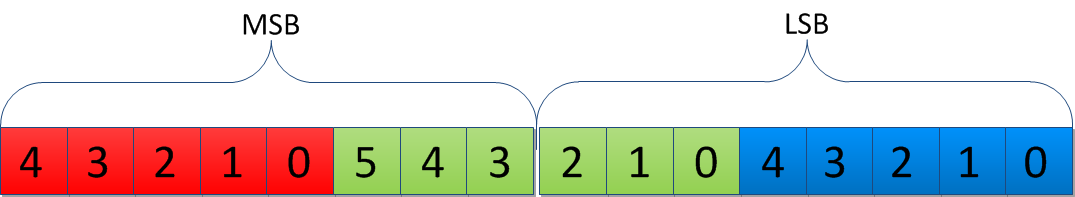
\includegraphics[width = \textwidth]{./Figures/RGB565.png}
\caption{RGB565 pixel format}
\label{fig:RGB565}
\end{figure}

The camera must use a high speed clock in order to ensure the pixels obtained are from the same time. This makes it difficult for an AVR to be able to respond to the camera quick enough (ATMegas typically clocked at 8-12MHz). This highlights the necessity for a FIFO Buffer. 

The OV7670 is set up so that the VSYNC pin goes low at the beginning of every full frame of data, and HREF is high when the data being output is valid. The pixel data is then clocked out on every rising edge of PCLK. To control the buffer, WEN (write enable) is NAND with the HREF signal. When both are high, the write enable to the buffer will be active and the data will be clocked in by PCLK. In order to acquire a full frame, the first VSYNC pin is set up to interrupt the AVR to enable WEN. The camera will output an entire frame of pixel data and store it into the buffer. When the second VSYNC is received, the WEN signal is disabled, stopping any more data being stored. The FIFO buffer now contains an entire image.

To obtain the data from the buffer, the AVR sets output enable and pulses the read clock. Valid data is available on the input port while RCLK is high. All the data is then read in half a pixel at a time. The entire operation can be seen in figure \ref{fig:ov_Capture}.
\begin{figure}
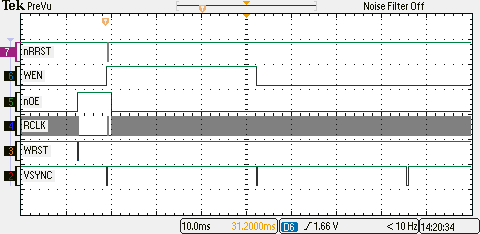
\includegraphics[width = \textwidth]{./Figures/ov7670_im_capture.png}
\caption{Signals generated to control the OV7670 capture and read}
\label{fig:ov_Capture}
\end{figure}


Difficulties arose at this point with the storage of the data. The ATMega644P has 4kB of internal SRAM, but  153.6kB of memory is needed to store a single image at QVGA (320 by 240 pixels, 2 bytes per pixel) quality. 

Firstly, data was sent straight to a desktop computer via a COM Port using USART. A simple desktop program was written in C\# to receive and store all the data, and to make a Bitmap image from the data. This method was slow, taking around 30 seconds to transmit one uncompressed image. 

The second option was to use extra memory connected to the microcontroller. An SD card is used as FAT file system so that data can be looked at by a user on a computer. Text log files are also written to aid debugging. This is discussed in section \ref{sect:SDCard}. 

\subsection{Dual Camera Operation}
In order for stereovision to be successful, two cameras separated by a horizontal distance ($B$) will need to be driven at the same time to obtain photos within a small time frame of one another.

A major problem occurred with using the \itc interface to set up both cameras. The camera has a set \itc address of $21_{16}$, which cannot be changed. Multiple \itc devices with exactly the same address cannot be used on the same bus. 
Two solutions to this are possible: driving one from $I^{2}C$ and one from SCCB, or using an \itc multiplexer. By using two different buses, there can be no bus contention. However, SCCB is slow and processor-hungry as it deals with the protocol bit by bit in software. This takes up memory and is not reusable for other operations.

An \itc multiplexer sits on the bus and has multiple output buses. The master can then address the multiplexer and select whether to pass the bus to bus 0, bus 1 or not allow the data to be transferred. This saves processor time, but means a write operation has to be done to select the camera bus before being able to write to the camera. This slows down the operation, but not as much as using SCCB. The main disadvantage to the \itc MUX is the extra hardware needed; firstly the MUX itself, but also 7 extra resistors to pull up the two extra buses and the three interrupt lines must be added. 

Overall, the disadvantages posed by using a MUX are small, so a multiplexer will be used as opposed to the SCCB interface. A suitable multiplexer is the Phillips PCA9542A \citep{I2C_Mux}.

The buffers have an output enable pin so the data bus can be shared by both cameras to the AVR. The ATMega644P offers three interrupt pins, two of which are used by the two VSYNC pins for the cameras.

Two ISRs are used to control the VSYNC signals, and when taking a photo, both frames are taken at a time period close together to capture the same scenario. The data for both images are read back individually by the AVR. 

Operation to read an image is identical to using one camera. However, an ID number is passed through the functions to make a decision on the pins to use to read the buffer and to enable the output. Care was taken to avoid bus contention, but no checking procedure is explicitly in place. Both images are then read back from the buffers and stored to memory. 

\section{SD Card} \label{sect:SDCard}

To use the SD card, the FATFS library \citep{FATFS} was used. The library supplies all the functions for writing a FAT File System in the files \textit{ff.c}, \textit{ff.h}, \textit{ffconf.h}, \textit{diskio.c}, \textit{diskio.h} and \textit{integer.h}. The \textit{diskio.h} functions control what device is being used - SD/MMC Card, USB drive etc. The \textit{ff.h} header contains all the functions to write to in a FAT File system. 
\\
An SD card was chosen due to it's small size, low cost and a large data storage. The cards work using an SPI bus which can be used for other devices within the system so the card only uses one extra enable pin in hardware to function. 

\subsection{Storing Images}

Many image formats are common, such as Joint Photographic Expert Group (JPEG), Portable Network Graphics (PNG), Bitmap (BMP) and Graphics Interchange Format (GIF). Table \ref{ImageFormats} shows a summary of some common image formats.


\begin{table}
\centering
\begin{tabular}{|p{3cm}| p{2cm}|p{2cm}|p{2cm}|p{2cm}|} \hline
			&	Bitmap 		& 	JPEG			 	&	PNG				& 	GIF \\ \hline
Extension 		& 	*.bmp 		&  	*.jpg /*.jpeg 		& 	*.png				& 	*.gif \\ \hline
Compression 	& 	No 			& 	Lossless  and Lossy		&	Lossless ZIP			&	Lossy	\\\hline
File Size of 320 by 
240 pixel Image (kB) &	225			&	20				&	23				&	24 \\\hline
Bits per Pixel		&	8, 16, 24 or 32	&	24				&	24, 32 or 48 			& 	24, but only 256 Colours \\


\hline
\end{tabular}
\caption{A table comparing different image formats available (\cite{ImageComparison})}
\label{ImageFormats}
\end{table}

It is clear that the best choice for images would be either PNG or JPEG. However, these require more computational time to compress the image into the correct format. To avoid compression, and thereby save processing time, bitmap was chosen at the expense of using more memory. The data in a bitmap image is also stored in RGB format so can be read back easily when processing the image. Appendix \ref{Chapter:AppendixB:BMPFile} shows the make up of a Bitmap File that was used.

By writing the image in this format, they are then able to be opened on any operating system. This aids debugging and allows the prototyping of image algorithms in a more powerful environment. Figure \ref{ExampleImage} shows a photo taken by the OV7670 and stored on a SD card.

\begin{figure}
\begin{center}
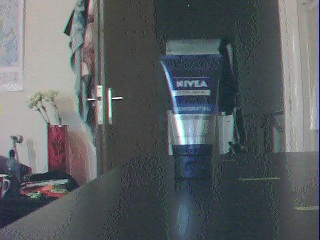
\includegraphics{Figures/ExampleImageFromCamera.jpg} 
\end{center}
\caption{An Example Image taken using the OV7670 and stored as a Bitmap on the SD Card}
\label{ExampleImage}
\end{figure}

\subsection{User Interface}
The ATMega 664P pinout for the dual camera operation can be seen in table \ref{table:644Pin}. Due to a lack of available GPIO pins, an ATMega168 was added on the \itc bus to act as a port extender. The ATMega168 accepts a read or write command. A write places the written data on Port D and a read returns any button pressed that occurred on Port C. When a button is pressed, this is stored in the ATMega168 until a read has been done. This is so the master (644P) does not miss any button presses while busy doing lengthy operations such as writing an image. The code is based on Application Note AVVR311 \citep{Atmel:I2CSlave}, written for IAR Compiler. This code was altered to compile with GCC under Atmel Studio. AVRs contain a hardware based \itc protocol that is interrupt based in software. The interrupt service routine of the TWI vector is a state machine which loads the data to send, stores received data, responds to acknowledges and address calls and deals with bus errors that can occur.

\begin{table}
\centering
\begin{tabular}{|c|c|c|c|c|}\hline
	& 	Port A 	& 	Port B 			& 	Port C 				& 	Port D 		\\ \hline
0	&	Data 0	&	SD Write Protect&	\itc - SCL			&	No Connection	\\
1	&	Data 1	&	SD Card Detect	&	\itc - SDA			&	No Connection	\\
2	&	Data 2	&	USB Data Plus	&	Read Clock 1		&	VSync 0			\\
3	&	Data 3	&	USB Data Minus	&	Read Reset 1		&	VSync 1			\\
4	&	Data 4	&	SPI Chip Select	&	Write Enable 1		&	Read Clock 0	\\
5	&	Data 5	&	SPI	MOSI 		&	Write Reset 1		&	Read Reset 0	\\
6	&	Data 6	&	SPI MISO		&	Output Enable 0		&	Write Enable 0	\\
7	&	Data 7	&	SPI Clock		&	Output Enable 1		&	Write Reset 0	\\
\hline

\end{tabular}
\caption{Pin Connections of the ATMega644P for Dual Camera Operation.}
\label{table:644Pin}
\end{table}
%\section{Motor Control}
%\inote{do something of this SOON}
\section{Circuit Development}
\subsection{Stereo Camera Development}
Figure \ref{sch:DualCam_Schematic} shows the circuit diagram for the prototype. This uses the Il Matto development board for the main microcontroller. The prototype can be seen in figure \ref{fig:Prototype}. This circuit captured and stored two images from the cameras to the SD card. 
\begin{figure}
\includegraphics[width=\textwidth]{./Figures/Prototype.jpg}
\caption{Prototype of Dual Camera operation.}
\label{fig:Prototype}
\end{figure}
\subsection{Motor Driver Development}
%\inote{Tachometers}
%\inote{Derivation of equations used - Distance / Rotating}
\inote{Testing of the Motor system - conclusion is likely to be that it is not a good method, need noise reduction}
\subsubsection{Hardware}
Tachometers are devices used to measure rotational speed of a shaft. Tachometers are most commonly found in bicycles where a small magnet is attached to the wheel and a sensor is attached to the frame. The sensor can then calculate the time period between rotations and therefore can calculate the speed (\citep{NEEDED}) \inote{Cite Needed}.

Here, an optosensor, TCRT1010, is used to measure rotations of the wheel and used to be able to move a distance decided by the microcontroller. The TCRT1010 package contains an IR LED and a phototransistor \citep{Vishay:TCRT1010:Datasheet}. The schematic of a simple transistor amplifier used can be seen in figure \ref{Circuit:TCRT1010} and was taken from \cite{NEEDED}. 
\inote{Cite Needed}
The wheel's rubber absorbed the IR, so a high voltage was always seen at the collector of the phototransistor. White tippex marks were applied to the wheels at regular intervals, which reflected IR and thereby giving a cheap way to detect wheel rotation. Figure \ref{Graph:WheelVoltage} shows the voltage at the collector (read by the ADC on the AVR) against the angle of the wheel. Five white tabs were marked on the wheel, and five dips in the voltage can be seen in figure \ref{Graph:WheelVoltage}. 

\inote{Maybe do some simulations of this circuit? This could dictate a maximum speed}

\begin{figure}
\centering
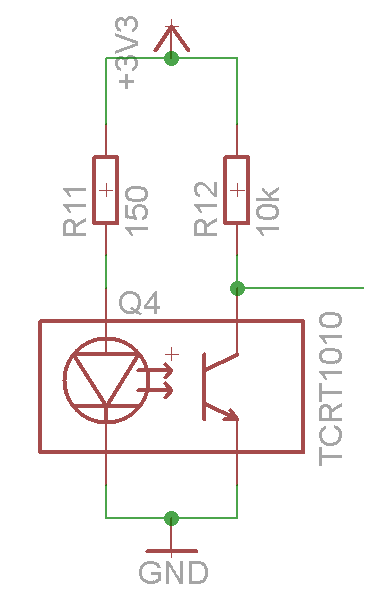
\includegraphics[scale=0.5]{Figures/TCRT_Circuit.png}
\caption{Circuit diagram of Optosensor}
\label{Circuit:TCRT1010}
\end{figure}

\begin{figure}
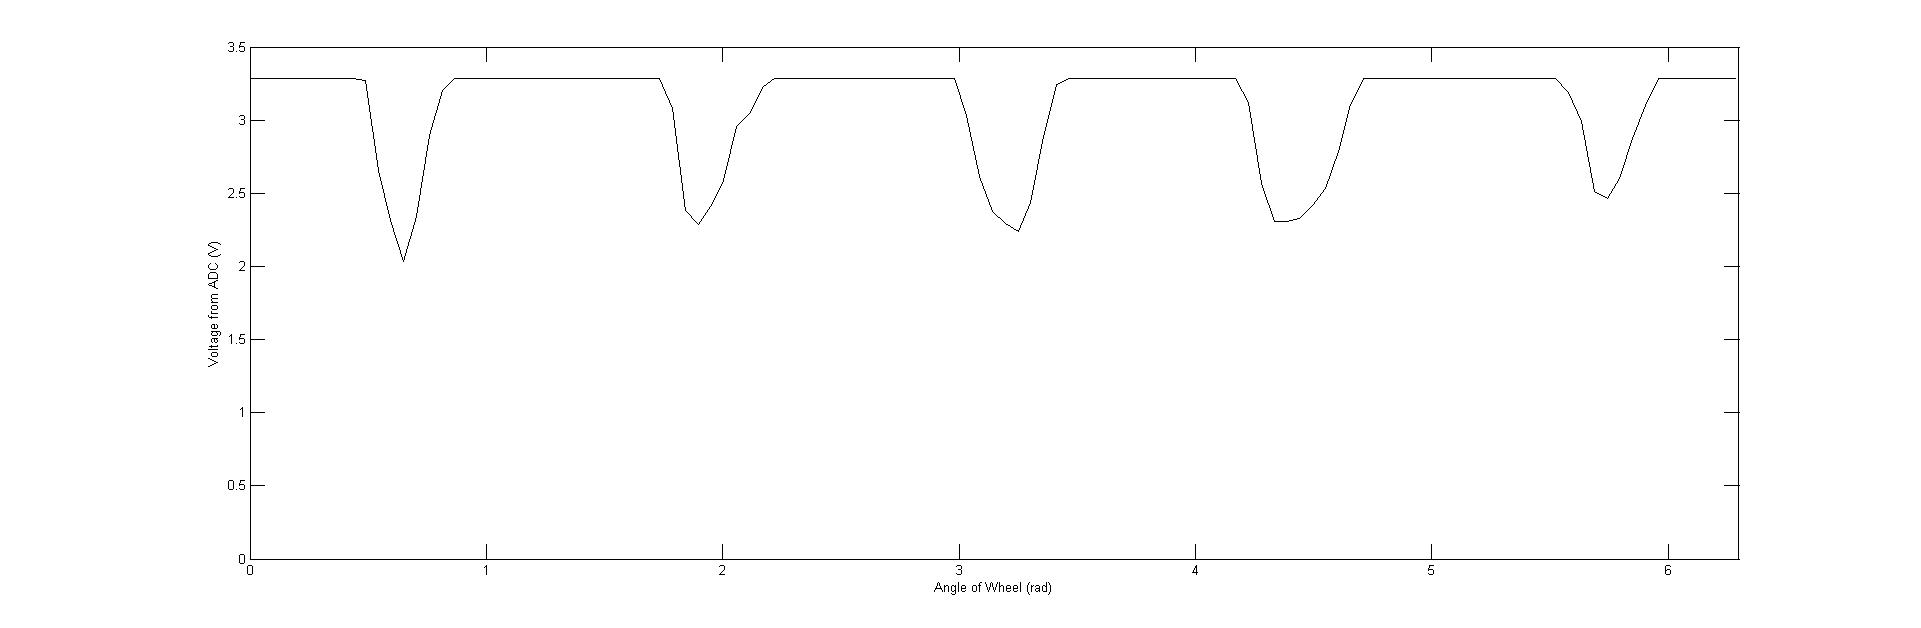
\includegraphics[width = \textwidth]{Figures/WheelVoltageGraph.jpg}
\caption{Graph of Wheel Angle against the Voltage read by the AVR}
\label{Graph:WheelVoltage}
\end{figure}

%\subsubsection{Derivations of Movement Calculations}
%Two basic movements were decided to be implemented: Straight line and rotation. 

\subsubsection{Firmware Development}

As the voltage swing from the phototransistor does not reach 0V, the AVR cannot detect this as a logical 0. The internal ADC can be used to continually read the analogue voltage from the phototransistor and detect low points from this data. This method requires the processor to continually compare values and process the data. However, more control would be had over the noise in the data.

An alternative is to use an analogue comparator built in on most AVRs. This can be set up to run an interrupt service routine when the voltage crosses a threshold. The threshold voltage can be determined by a potentiometer. The code is primarily two methods, the set up and the ISR.

Set up is different for if a rotation or movement is wanted. Moving in a straight line takes a parameter of how far to move as a signed integer and calculates the total number of interrupts that need to occur can be calculated using \eqref{eq:NumberInterrupts}. This value is put in a global variable. The PWM and input pins to set the correct direction are then set up before enabling the motor. 

\begin{equation}
\label{eq:NumberInterrupts}
Interrupts = D \times \frac{IPR}{C_w}
\end{equation}

To rotate, one of three methods can be used: Spot rotation on the centre of the robot, or pivot on either left or right wheel. For ease, the Spot rotation is the only one implemented. To calculate the distance moved, the radius to the wheels needs to be known. The circumference through the wheels is then easily calculated and the angle of rotation is then a ratio. The distance to move is calculated by equation \eqref{eq:RotationalDistance} and the total number of interrupts can be calculated using equation \eqref{eq:NumberInterrupts}. To rotate clockwise, the left motor is driven forward and the right is driven backwards. To rotate anti-clockwise, the directions are reversed

\begin{equation}
\label{eq:RotationalDistance}
D_{R} = A \times \frac{C_b}{360}
\end{equation}

Combining equations \eqref{eq:NumberInterrupts} and \eqref{eq:RotationalDistance} gives:
\begin{equation}
\label{eq:RotationalInterrupts}
Interrupts = A \times \frac{IPR}{C_w} \times \frac{C_b}{360}
\end{equation}
Where $A$ is the angle to rotate in degrees, $IPR$ is the number of interrupts generated per full revolution of the wheel, $C_w$ is the circumference of the wheel and $C_b$ the $2\pi\times r_b$ and $r_b$ is the distance from the centre of the robot to the centre of the wheel (see figure \ref{fig:RobotBase_Annotated}).



\begin{figure}
\centering
\subfigure[Top View of robot base showing dimensions of interest\label{fg:RobotBase:Top}]{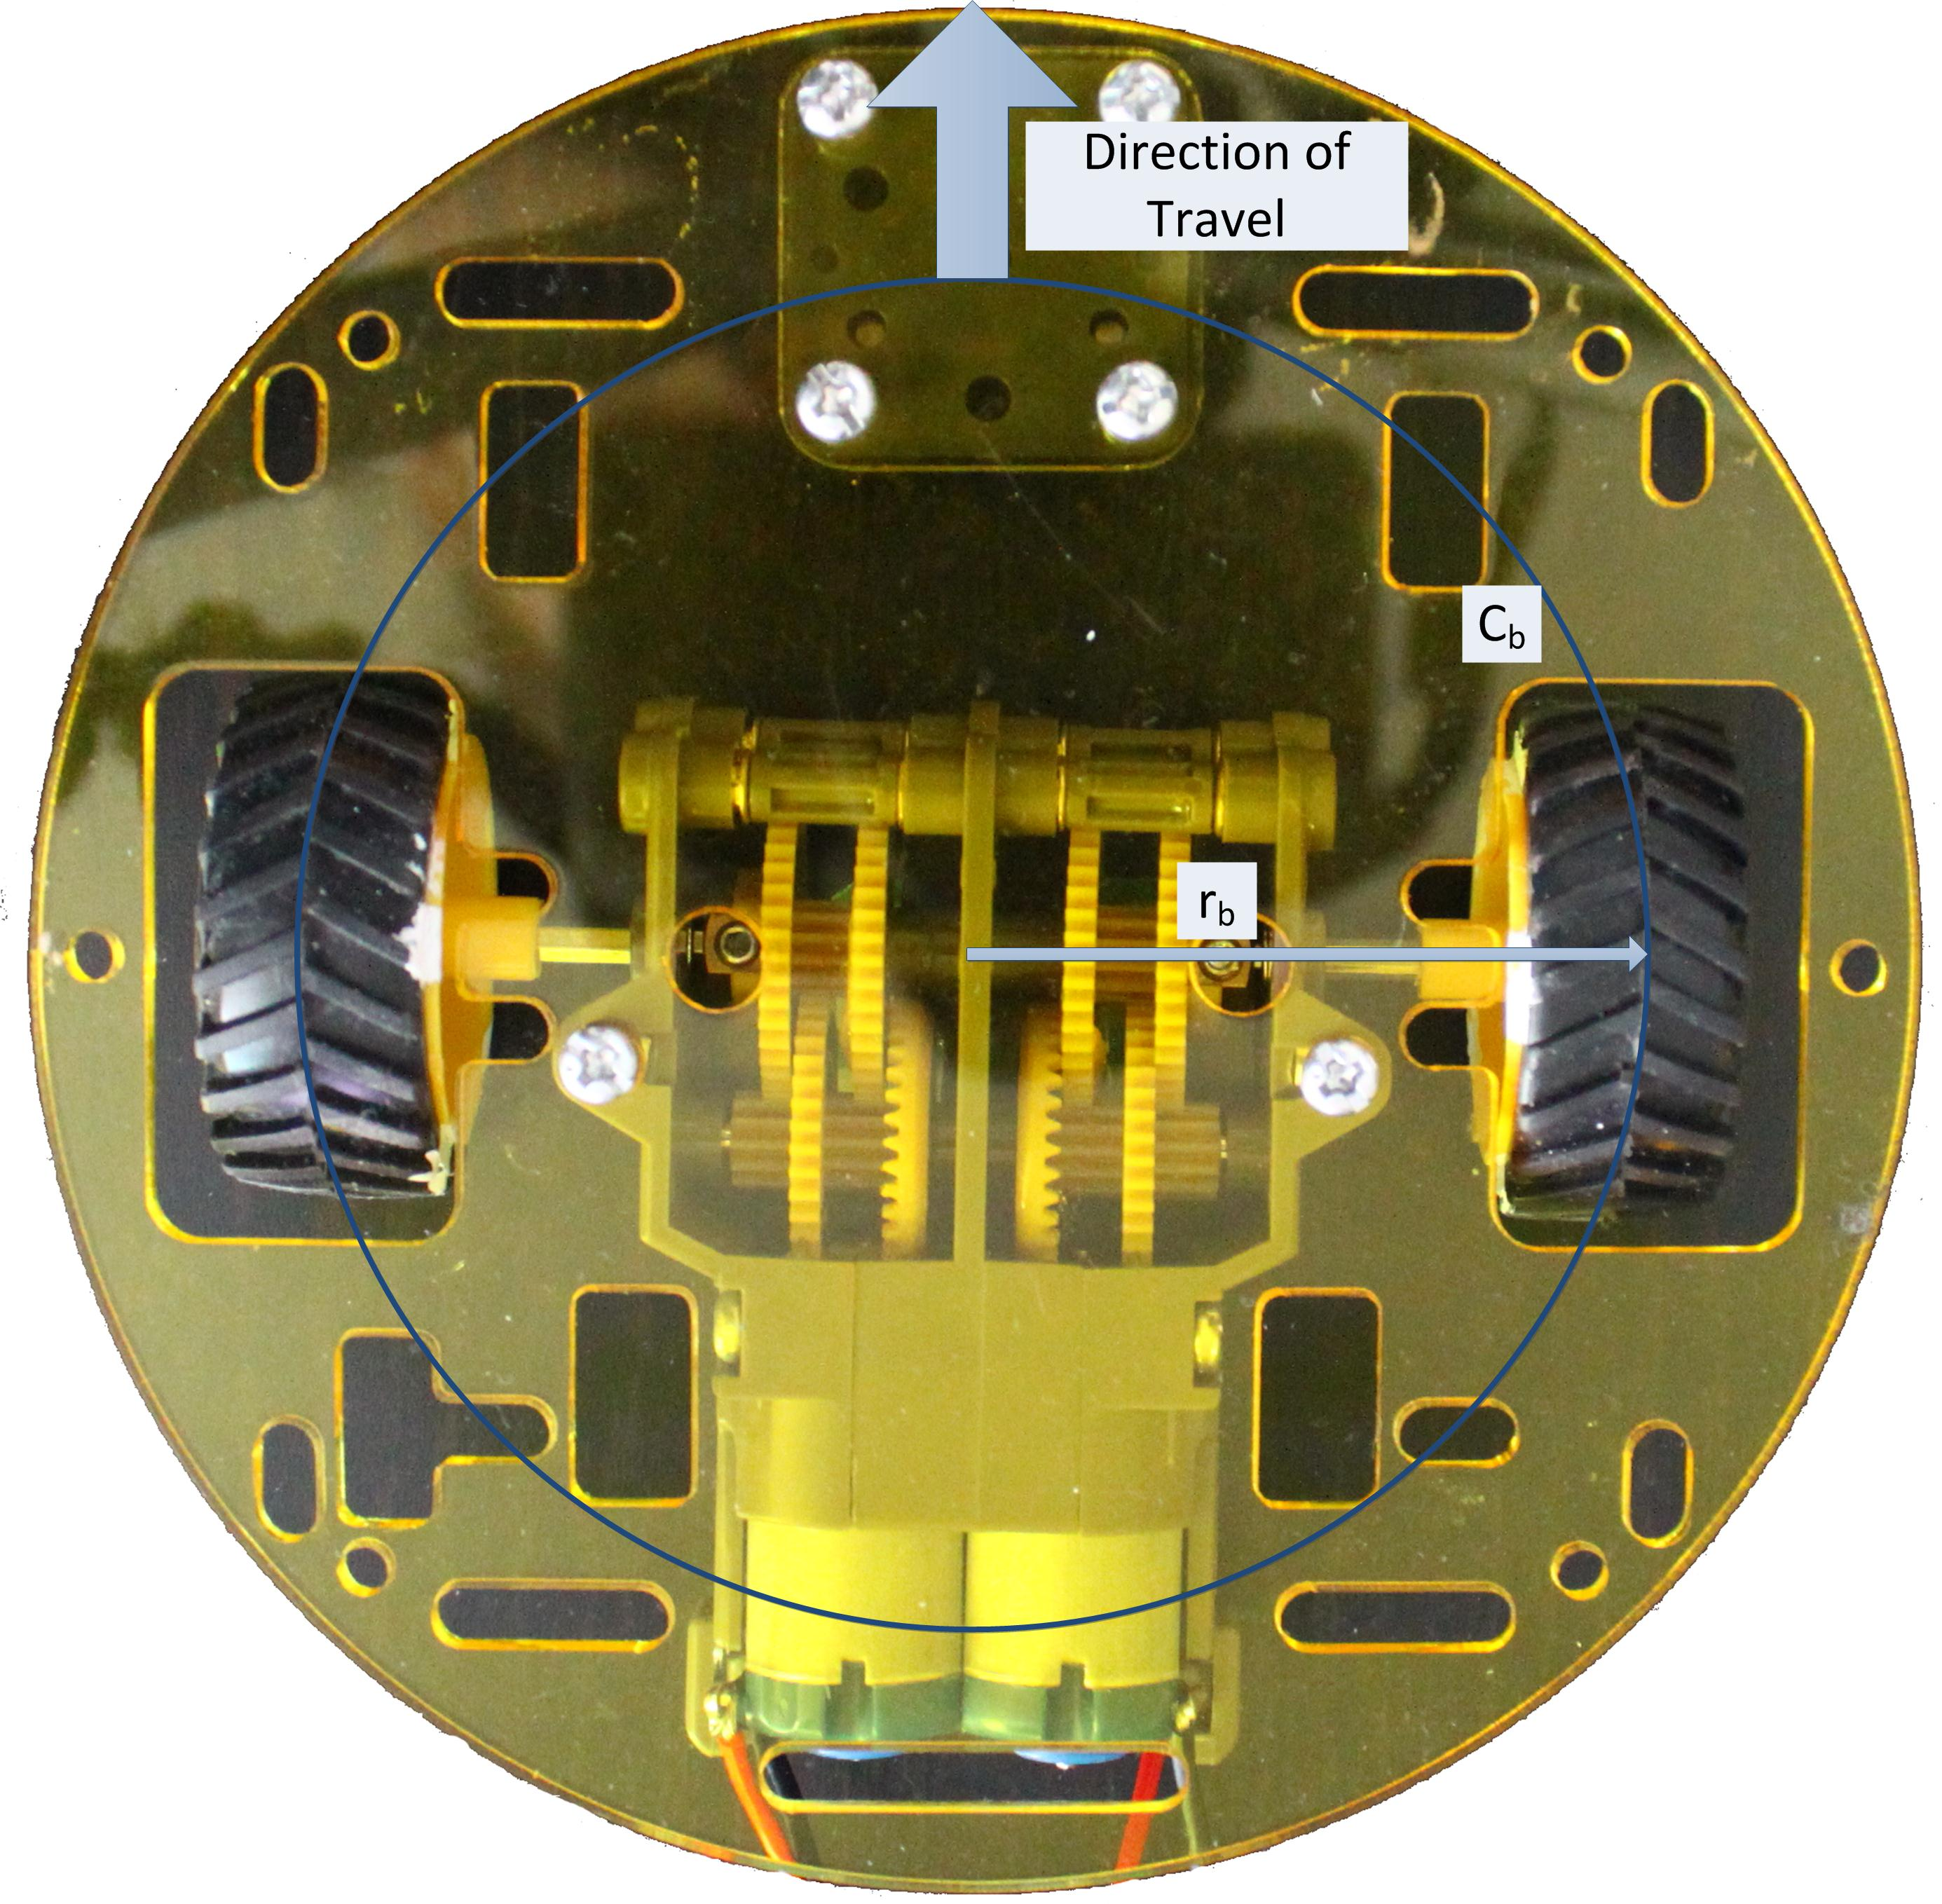
\includegraphics[width = \textwidth, keepaspectratio]{./Figures/Robotbase_top_annot.jpg} }
\subfigure[Side View of robot base showing dimensions of interest\label{fg:RobotBase:Side}]{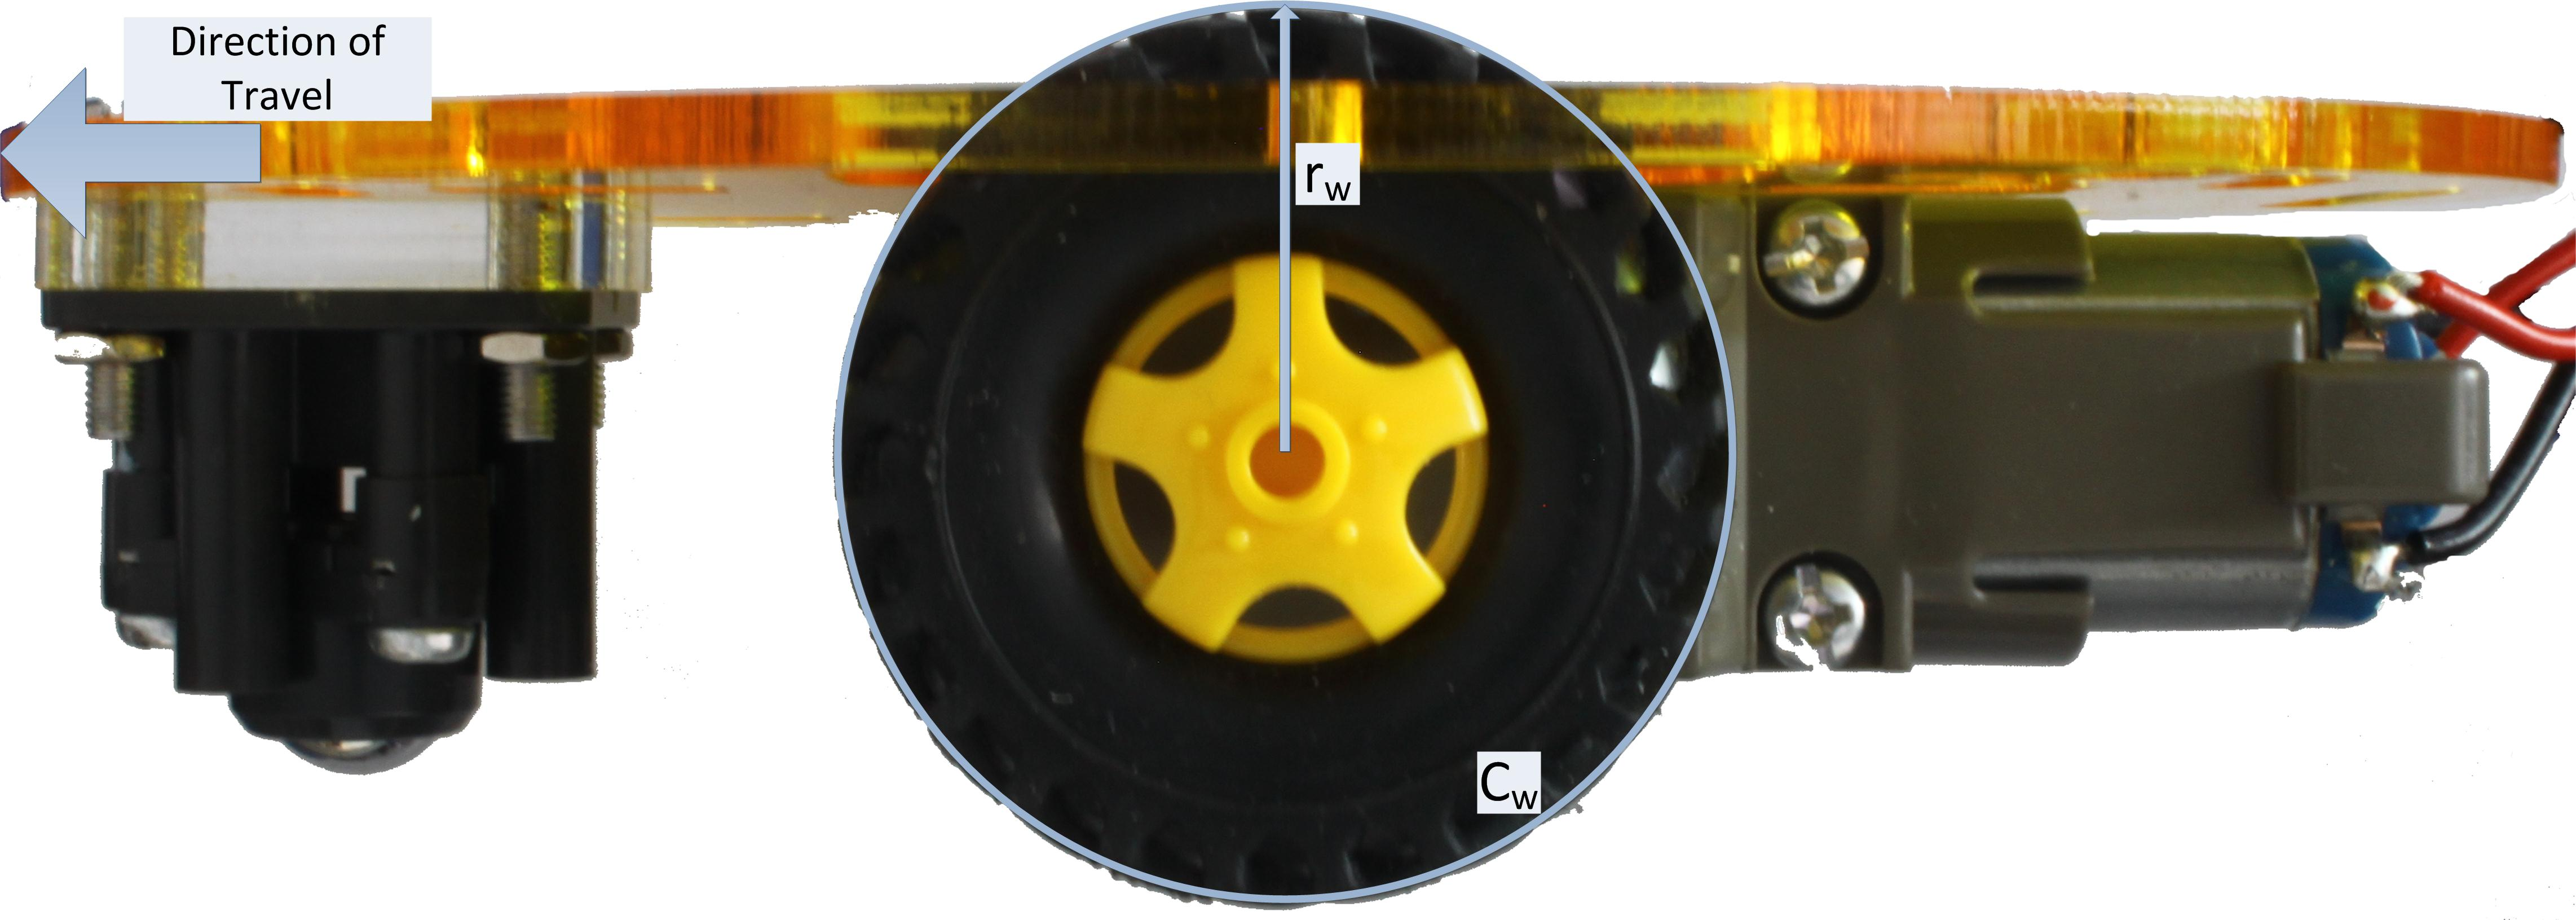
\includegraphics[width = \textwidth, keepaspectratio]{./Figures/Robotbase_side_annot.jpg} }
\caption{Dimensions of Interest for Robot Movement}
\label{fig:RobotBase_Annotated}
\end{figure}
\inote{Maybe a figure to explain better?}


The motor speed can be controlled by Pulse Width Modulation (PWM). The code sets up a low duty cycle PWM signal to drive the motors slowly. This removes the need for a controller to ensure the correct distance was moved. 

The final code can be seen in appendix \ref{Chapter:AppendixC:Code}
\subsubsection{Testing}\label{Section:MotorTest}
\inote{Need to get the motors to work reasonably first}
\subsubsection{Conclusion}
\inote{It doesn't work}

\section{PCB Development}
\subsection{Circuit Design}
The circuit diagram for Revision A can be seen in section \ref{sch:Columbus:CircuitDiagram}. The schematic for the SDRAM and values and locations of decoupling capacitors were taken from the schematic of the UC3C-EK development board \citep{Atmel:UC3CEK}. 
\subsection{PCB Design}
The PCB was designed using EAGLE CAD Software. A four layer board was decided to be used to save space when routing Power. Layer 2 is a 3V3 plane and layer 3 is a ground plane. A ground plane is also on the top and bottom layers to help eliminate any ground bounce that could occur. 

The SDRAM uses the EBI protocol. In high speed systems, care is often taken to equalise track lengths \citep{liu2004equalization}. The UC3C maximum clock frequency is 33MHz (with no wait states), which is not fast enough to cause any track equalisation problems. Care, however, was taken on the USB lines to ensure correct impedance and the tracks lengths matched to each other.

Tracks were routed in order of priority, starting with the UC3C, SDRAM and cameras, and then other devices were routed, \itc MUX, SD card, motor drivers etc. As a precaution, spare pins from the UC3C were routed to a header (J8 and J9) so that additions could be done if a pinout or connection was found to be incorrect. Also, UART, \itc and SPI connections were routed to headers J7, J4 and J5 respectively so logic analysers and COM Port could be attached easily for debugging.

Most of the passives used were 0603 size, but some 1206 capactitors were used for decoupling the voltage regulator and a 1206 diode was used for the analogue reference circuitry. LEDs were also 1206 size. All headers were 0.1'' spaced and a mini B USB socket was used. 

The layout of components was important. The cameras needed to be as far apart as possible and at the front of the PCB. The motor drivers were situated toward the back of the PCB and 0.1'' headers were added to connect the motors to. The optosensors were positioned such that they could be mounted directly on the PCB and be in the correct position to sense the wheels. Mounting holes were also added onto the board so the PCB could be mounted on to the robot base easily. The overall dimensions of the PCB were $100mm \times 70mm$. A full list of components and cost of each is documented in table \ref{table:Costings}


\begin{table}
\centering
\begin{tabular}{|c|p{2cm}|c|c|c|} \hline
Component	&	Cost per unit (\pounds)	& Quantity 	&	Cost (\pounds)	&	Source		\\ \hline
Capactiors	&	0.155 					& 	43		& 	6.67 					& 	Farnell 	\\
Clock 		& 	1.48					& 	1		&	1.48 					& 	Farnell		\\
Diode		&	0.48					&	1		&	0.48					&	Farnell 	\\
Headers		&	0.51 					&	5		&	2.55					&	Farnell 	\\
I2C Mux PCA9542A &	0.81				&	1		&	0.81					&	Farnell		\\
LEDs 		&	0.158					&	7		& 	1.11 					&	Farnell		\\
Micro SD Card &	4						&	1		&	4.00 					&	Amazon 		\\
Micro SD Card Connector & 2.04			&	1		&	2.04					&	Farnell		\\
AT32UC3C0512C	&15.39					&	1		&	15.39					&	Farnell		\\
TB6593FNG 	&	1.07 					&	2 		&	2.14 					&	Farnell 	\\
Motors  	&	0.42					&	2		&	0.84				 	&	Rapid 		\\
TCRT1010	& 	0.94 					&	2		&	1.88 					&	Farnell 	\\
OV7670		&	17						&	2		&	34.00					& 				\\
Potentiometer	&	0.43				&	2		&	0.86					&	Farnell 	\\
Resistors	&	0.066 					& 	46		&	3.04 					&	Farnell 	\\
MT48LC4M16A2P	& 3.24  				& 	1		&	3.24 					&	Farnell		\\
Switch		&	0.45					&	1		&	0.45					&	Farnell 	\\
USB Socket	&	0.84 					&	1		& 	0.84 					&	Farnell 	\\
LM1117MP	&	1.03					&	1		&	1.03	 				&	Farnell		\\ \hline \cline{3-4}
\multicolumn{2}{c|}{ }					& Total Cost  & \pounds 82.84			&	\multicolumn{1}{|c}{ }			\\ \cline{3-4}
\end{tabular}
\caption{A table of all components used and their costs.}
\label{table:Costings}
\end{table}

Finally, the name ``The Columbus'' was decided on as the original application for the project was a mapping robot that would search out an unknown area, so the robot was named after Christopher Columbus who explored and navigated parts of the American continents which were unknown at the time. The Eagle CAD Diagram of the PCB can be seen in Appendix \ref{Appendix:PCB}. The PCB was manufactured by \cite{PCBCart}. The PCB cost \pounds 205 to manufacture and ship. A photo of the PCB can be seen in figure \ref{fig:PCB:Bare}. 

\begin{figure}
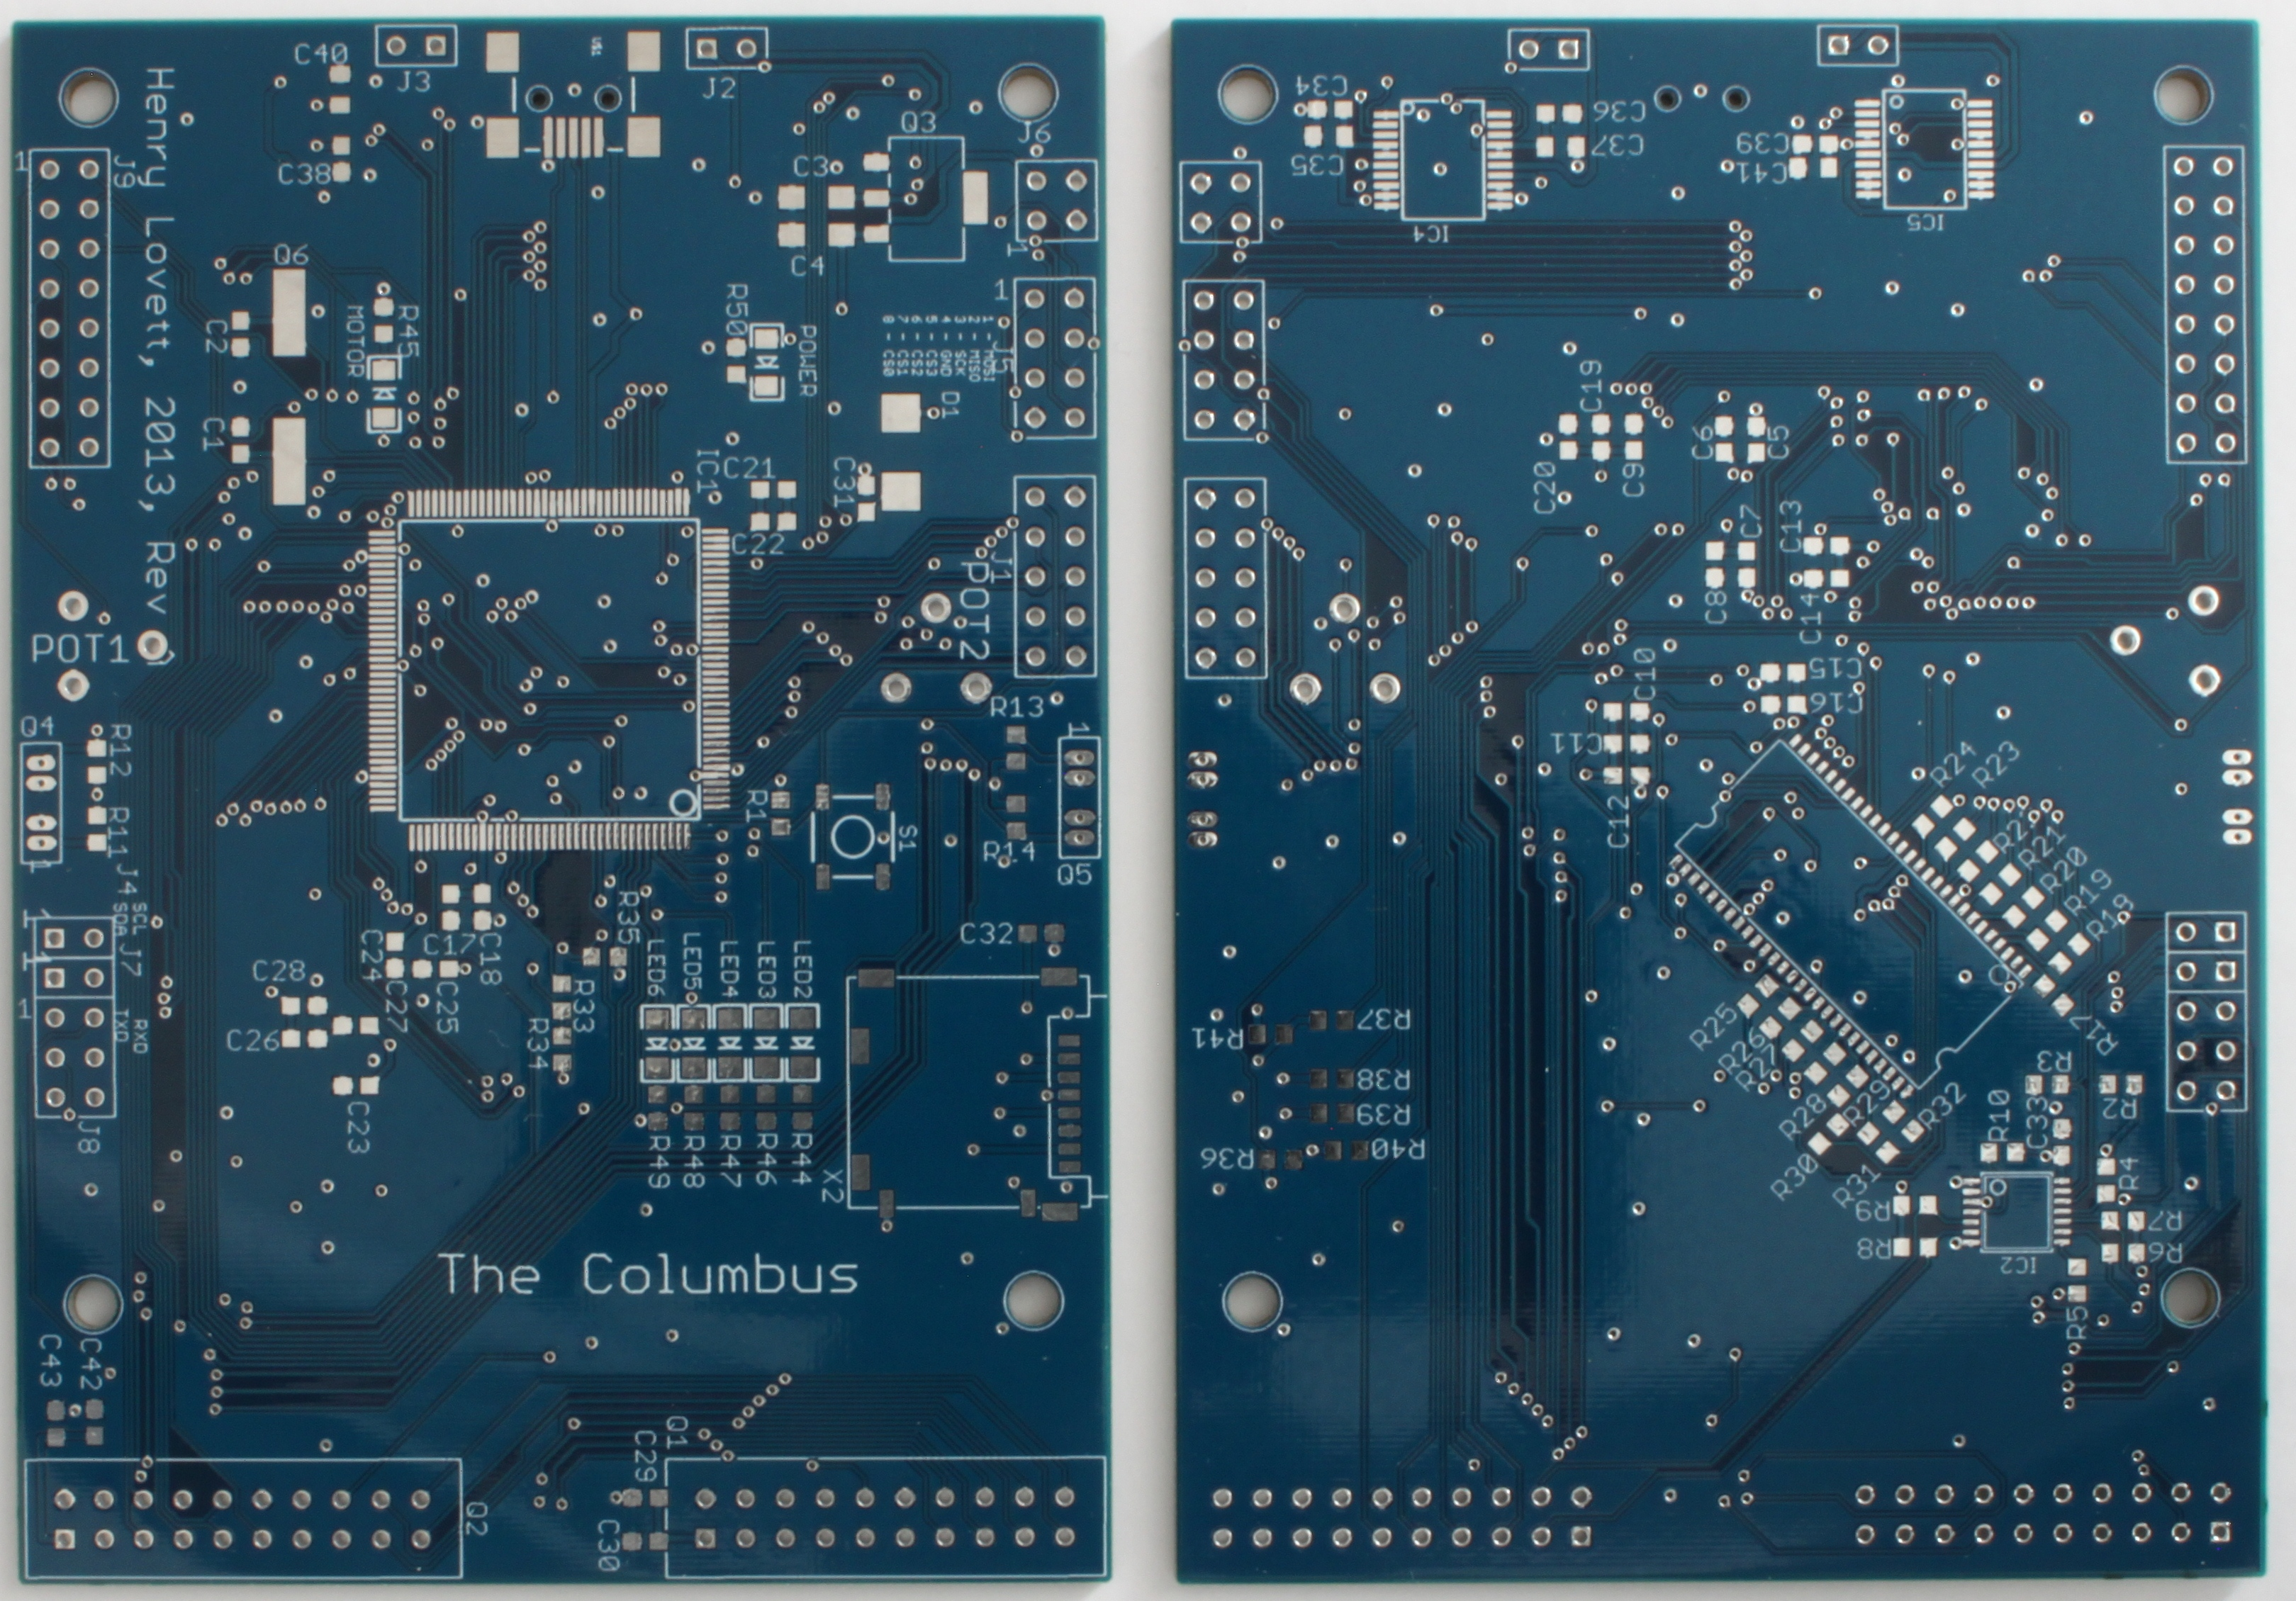
\includegraphics[width=\textwidth]{./Figures/PCB_Bare.jpg}
\caption{PCB with no components. Left: Top View. Right: Bottom View}
\label{fig:PCB:Bare}
\end{figure}

\inote{Considerations - Power consumption of devices not exceeding VReg}

\subsection{PCB Testing}
A program was written to test all the devices on the PCB. The following tests are done:
\begin{enumerate}
\item UART Send and Receive
\item SD Card Test
\item All LEDs on and off
\item SDRAM Test
\item \itc Test
\item Camera Test
\item Motor Test
\end{enumerate}
The folowing sections explain the tests done to check the devices and protocols worked.

\subsubsection{UART Test}
When the test program begins, the microcontroller waits for a character input. All characters are echoed back. This enables the user to check the communications work. Once a carriage return key is received ($13_{10}$), the test program continues. Listing \ref{lst:UARTTestCode} shows the test code for the UART protocol.

\lstinputlisting[style=C,caption=UART Test Code,label={lst:UARTTestCode},frame=single,numbers=left,tabsize=2,breaklines=true, firstline=110,lastline=121]{../Code/ColumbusTest/ColumbusTest/src/main.c}


\subsubsection{SD Card Test}
The Atmel Software Framework \citep{Atmel:ASF} provided drivers and code for SPI communications and use of a FAT32 File System. The code was configured to use the correct Chip Select pin for the SD Card and the correct SPI Bus was also configured. The test consists of initialising the memory, reading the capacity of the card and printing it to the user. 

The AVR then proceeds to delete any previous log file, create a new log file and writes \textit{``Columbus Tester''} to it. The first 8 characters, which should be \textit{``Columbus''} are read back and checked.
\lstinputlisting[style=C,caption=UART Test Code,label={lst:SDTestCode},frame=single,numbers=left,tabsize=2,breaklines=true, firstline=124,lastline=196]{../Code/ColumbusTest/ColumbusTest/src/main.c}

This exercises all basic File I/O functions, creating, reading and writing and checks them on the device.

\subsubsection{LED Test}
All LEDs are turned on for 1 second, and then turned off. The user should check this occurs. It verifies that all the LEDs are functional and correctly mounted. The Power LED should be on when power is supplied to the PCB. 

\subsubsection{SDRAM Test}
The SDRAM test consists of initialising the SDRAM, calculating the SDRAM Size, writing a unique test pattern to the whole memory, and then reading it back and checking it. The total number of errors are reported. 

The test was adapted from an Example Application from the Atmel Software Framework \citep{Atmel:ASF}. The code can be seen in listing \ref{lst:SDRAMTestCode}. It consists of two \textit{for} loops. In the first, the iteration number is assigned to the memory location. The second loop reads back the data and checks it is correct. An int, \textit{noErrors}, is used to count errors. 

\lstinputlisting[style=C,caption=SDRAM Test Code,label={lst:SDRAMTestCode},frame=single,numbers=left,tabsize=2,breaklines=true, firstline=217,lastline=258]{../Code/ColumbusTest/ColumbusTest/src/main.c}

\subsubsection{\itc Test}
The \itc test checks the bus for devices. It prints out a table showing the address of any devices that acknowledge a probe. A probe is a set up to write to the address. If a device exists on the line, it should Acknowledge \citep{Philips:I2C}. The test is done three times, with no channel selected on the \itc MUX, with channel 0 selected and with channel 1 selected. The two addresses expected at $21_{16}$ for the OV7670 Camera and $74_{16}$ for the \itc MUX. The camera should only acknowledge when the \itc MUX has the relevant channel selected. Listing \ref{lst:TWITestCode} shows the test code for the \itc bus and listing \ref{lst:TWITestCode} shows the result from the full bus scan with channel 0 selected. The cameras are both checked to exist.
\lstinputlisting[style=C,caption=\itc Test Code,label={lst:TWITestCode},frame=single,numbers=left,tabsize=2,breaklines=true, firstline=268,lastline=315]{../Code/ColumbusTest/ColumbusTest/src/main.c}

\begin{lstlisting}[caption={Result of \itc bus scan with Channel 0 of the \itc MUX selected},label={lst:I2CTest}]
Scanning Channel 0
h 0 1 2 3 4 5 6 7 8 9 A B C D E F
0 - - - - - - - - - - - - - - - -
1 - - - - - - - - - - - - - - - -
2 - A - - - - - - - - - - - - - -
3 - - - - - - - - - - - - - - - -
4 - - - - - - - - - - - - - - - -
5 - - - - - - - - - - - - - - - -
6 - - - - - - - - - - - - - - - -
7 - - - - A - - - - - - - - - - -
\end{lstlisting}

\subsubsection{Camera Test}

This test consists of initialising both cameras and checking it passes. Two photos are then taken and stored to the SD card. Success or Failure is displayed. Two images should exists on the SD card from the two cameras. Listing \ref{lst:CameraTestCode} shows the code to conduct this test.
\lstinputlisting[style=C,caption=Camera Test Code,label={lst:CameraTestCode},frame=single,numbers=left,tabsize=2,breaklines=true, firstline=316,lastline=338]{../Code/ColumbusTest/ColumbusTest/src/main.c}

\subsubsection{Motor Driver Test}
An extensive test of the motor driver is discussed in section \ref{Section:MotorTest}. The test code in this application resets the motors so that they are aligned to a white tab on the wheel. This code can be seen in listing \ref{lst:MotorTestCode}. The robot should move no further than 2cm to reach a white tab and the motors should drive forward. This test is useful here to ensure the motors are connected the correct way around and that the potentiometers are set to an appropriate level.

\lstinputlisting[style=C,caption=Motor Test Code,label={lst:MotorTestCode},frame=single,numbers=left,tabsize=2,breaklines=true, firstline=339,lastline=346]{../Code/ColumbusTest/ColumbusTest/src/main.c}

\subsection{PCB Faults}
During the build and test of the PCB, a number of faults were found. Each is explained and the solution for the problem given. 
\subsubsection{SDRAM Footprint}
The SDRAM footprint made was done exactly to the specification of the pad size and locations with no consideration for soldering to. This meant the chip fit exactly on to the footprint. This made soldering difficult as pads had to be preloaded with solder and the device's pins were heated and bound to the solder. The chip does not seat flat against the PCB. It also put the device at risk as more heat had to be used that usually necessary. Figure \ref{fig:SDRAM_Err} shows the SDRAM chip against the footprint. There is no extra space on the pad to be able to easily solder the device.

\begin{figure}
\centering
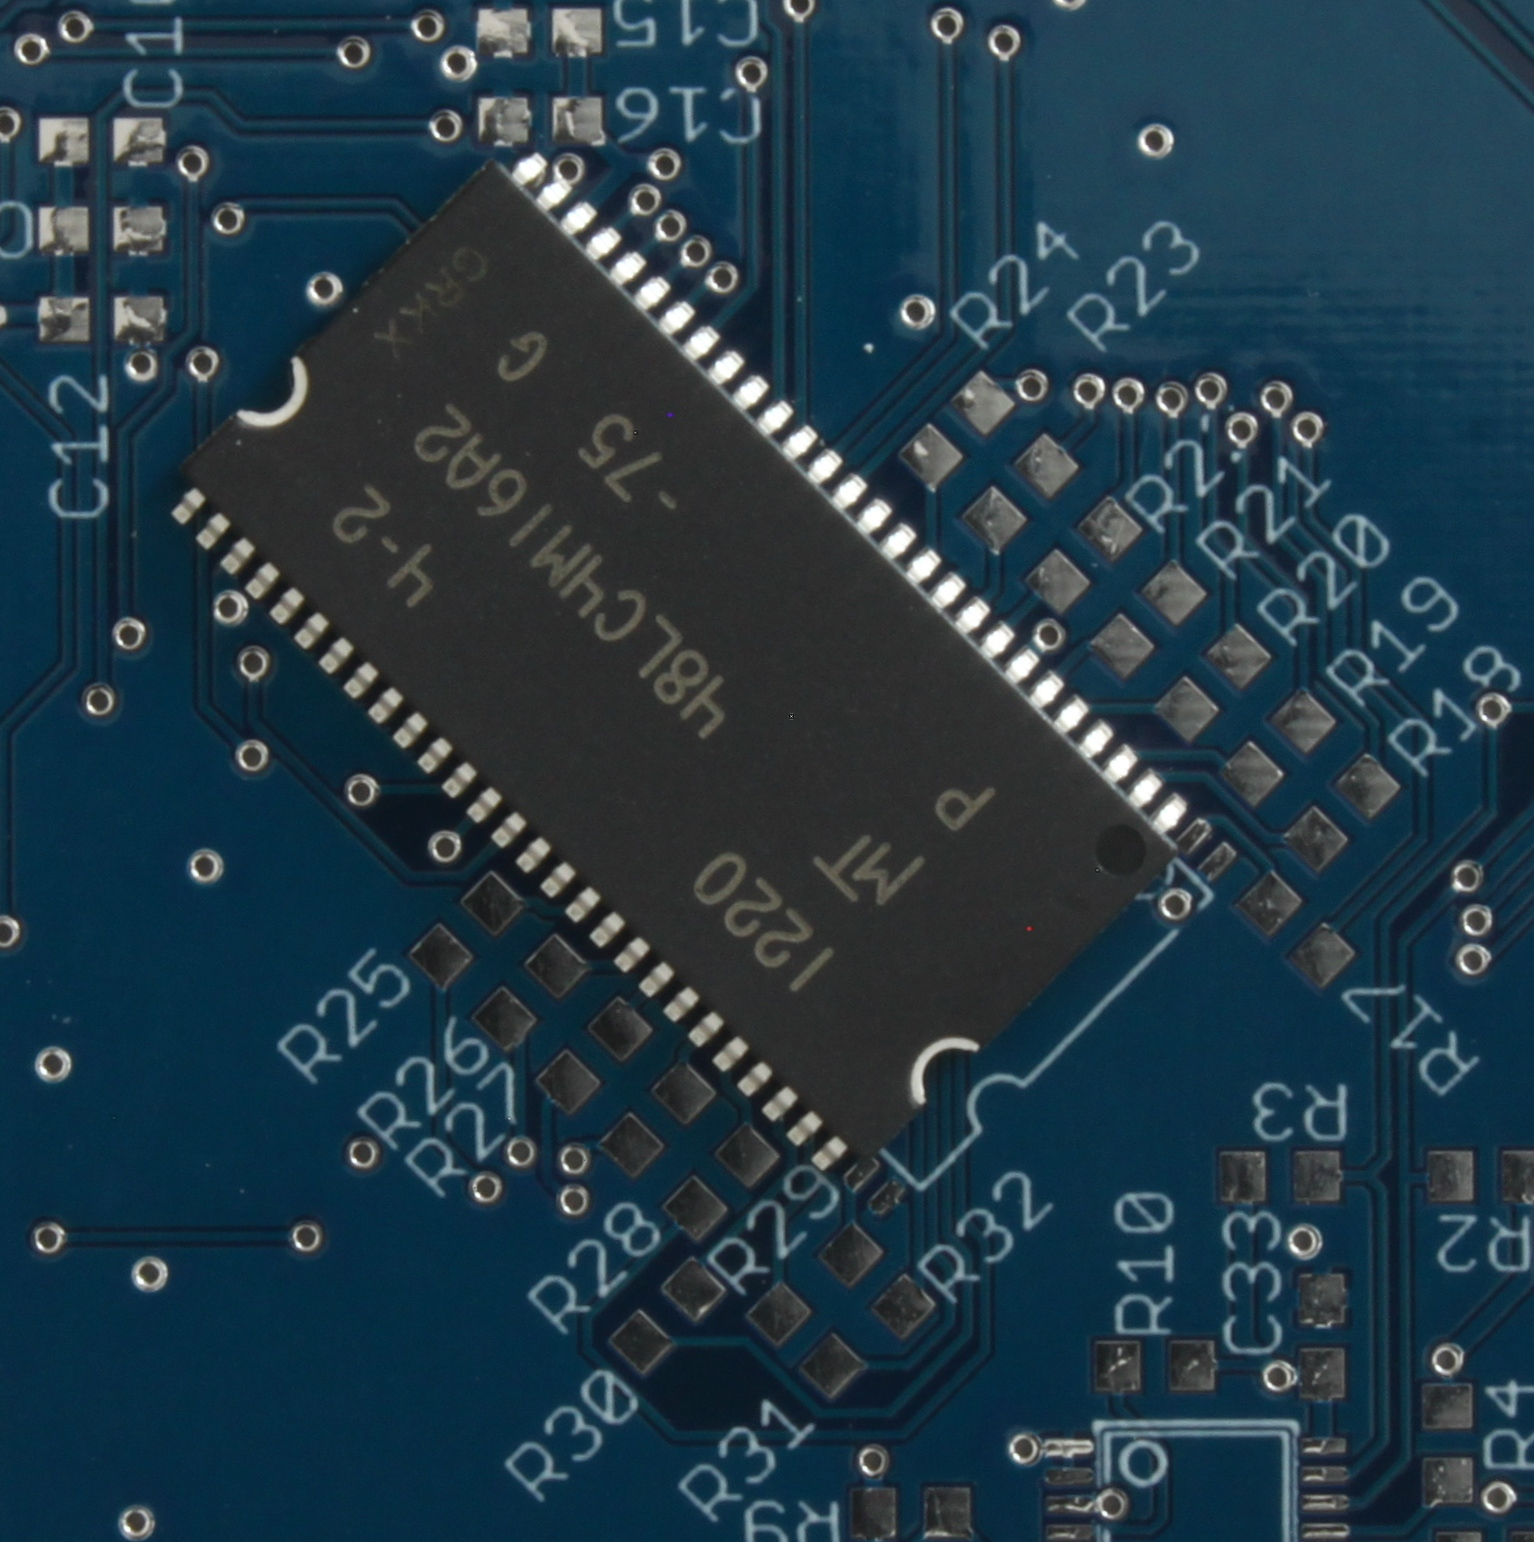
\includegraphics[width=\textwidth / 2]{./Figures/PCB_SDRAM.jpg}
\caption{SDRAM Chip shown against its footprint.}
\label{fig:SDRAM_Err}
\end{figure}

To avoid this, existing footprints could be used from other libraries, or double checking the footprints made. The problem meant extra care during soldering had to be taken but has not impeded the operation of the device. 

\subsubsection{SDRAM Chip Select}
The code was prototyped on the Atmel UC3C-EK development board prior to the PCB arriving. When the PCB was built, the code did not work, even with the Chip Select declaration changed. To diagnose this problem, the control lines of the SDRAM were probed with a logic analyser. On the UC3C-EK, the bus was busy with refresh cycles outside of SDRAM access. On the Columbus, no activity was seen. 

The reason the correct control wasn't being seen was due to the UC3C device having a dedicated SDRAM controller, attached to only Chip Select line 1. The Columbus was designed to used chip select line 0. Chip select 1 was available on an external pin, and a via through the routing was close to a via connected to the SDRAM chip select line. Therefore, to overcome the problem, a small enameled wire was soldered to join the two vias together. This solved the problem and the correct signals were then seen on the control lines. The patch can be seen in figure \ref{fig:PCB:Bottom}. 

This fault was caused by not reading the datasheet carefully and ignoring a proven circuit diagram. 

\subsubsection{SDRAM Data Line Resistors}
Once the chip select problem was solved, data returned was unreliable. The SDRAM is word (32 bit) addressed, but accessed in 16 bits. This means read cycles are done per word read. 
Upon investigation of this problem, the 14th, 15th, 30th and 31st (top two bits of each 16 bit access) seemed to read as a 1 the majority of the time. This result wasn't repeatable and sometimes returned correct data. The other bits of the data were always correct. Table \ref{table:SDRAM_Err} shows some examples of the problematic data bits. The data written should match the data read back. 

\begin{table}[!ht]
\caption{A table showing examples of the incorrect data returned from the SDRAM}
\label{table:SDRAM_Err}
\begin{tabular}{c c}
Data Written							&	Data Read \\
00000000 00000000 00000000 00000000		&	\textcolor{red}{11}000000 00000000 \textcolor{red}{11}000000 00000000 \\
00001111 00001111 00001111 00001111		&	\textcolor{red}{11}001111 00001111 \textcolor{red}{11}001111 00001111 \\
\end{tabular}
\end{table}

The problem was traced to resistors \textbf{R31} and \textbf{R32}. They were soldered on incorrectly so that the two data lines of the SDRAM were connected together and the two AVR GPIO pins were connected together. Data was then read back from, effectively, a high impedance line and therefore varied. Once the resistors were soldered correctly, the issue no longer persisted and the whole SDRAM test passed. By utilising the soldermask more, device orientations could be added to ensure correct placement. This can be extended to other devices, such as diodes and capacitors, especially in densely populated areas. 

\subsubsection{Camera Interrupt Line}

As discussed in section \ref{Section:Camera}, the OV7670 needs an interrupt line to synchronise quickly to the start of the frame and is done by using an interrupt line. The UC3C0512C has 9 external interrupt lines. On the PCB, interrupt lines 0 and 1 were used for this control.

Interrupt line 1 was easily configured and worked as expected. However, interrupt 0 did not seem to trigger the interrupt service routine. It was found that interrupt 0 was a ``Non Maskable Interrupt'' which has specific uses and cannot be used in to trigger a method. 

The external interrupt 4 pin was wired to Junction 8 on the PCB. A wire was attached to the camera's VSYNC line and attached to the relevant pin on the header. The operation was then easily obtained and the VSYNC line triggered correctly.

This issues would have been avoided with more understanding of the device before hand and checking the datasheet.


\subsubsection{Motor Driver Pinout}

An error was made in creating the device for the TB6593FNG Motor Driver in EAGLE. On the device, each motor output has two pins to drive each side of the motor. The pin assignment was mixed up when created and connected the two outputs together. Figure \ref{fig:Motor:Error} shows the track errors on one of the motor drivers. 

\begin{figure}
\centering
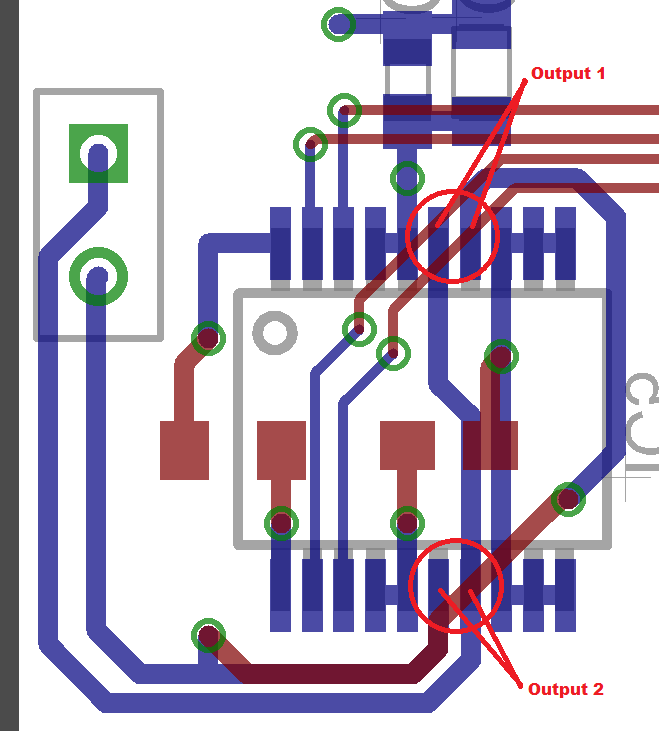
\includegraphics[width = \textwidth /2]{./Figures/MotorDriver_error.png}
\caption{Motor Driver error. Outputs incorrectly connected}
\label{fig:Motor:Error}
\end{figure}

To solve this, pins 7 and 14 were lifted and removed so that output 1 and output 2 were not connected together. The devices were not damaged in the process of testing this and the motors functioned correctly after this. Double checking the footprints made against the datasheet would have avoided this problem. No impedance to the operation of the drivers has been seen, but the patch may hinder the devices ability to sink current to the motors. 

\subsection{PCB Conclusions}
A number of faults were made in the PCB design. They are:
\begin{itemize}
\item SDRAM footprint
\item SDRAM chip select line
\item SDRAM data line resistors
\item Camera interrupt line
\item Motor driver pinout
\end{itemize}
Three of the faults could have been avoided by consulting the datasheet more carefully during the circuit design stage. The footprint error was due to not being experienced in designing footprints and the data line resistors was a mistake due to lack of attention being paid. 

For future PCBs, more care will be taken in circuit design, with prototyping of circuits with the hardware that will be used. This will highlight any pin specific operations (e.g. the non maskable interrupt) and reduce debugging post production. The effectiveness of a soldermask is also apparent, so more time spent on utilising this would be helpful during assembly.

The PCB itself, was a success. It was a complex PCB with many potential things that could have gone wrong. It was the first PCB I had designed and was a four layer board, using some devices that I did not have experience with. All devices are functional (with a few small modifications) on the PCB so firmware development could continue with all hardware able to be used.

\section{Conclusions}
\inote{Overall Conclusions of the Hardware design}
\begin{figure}
\centering
\subfigure[Top view of built PCB\label{fig:PCB:Top}]{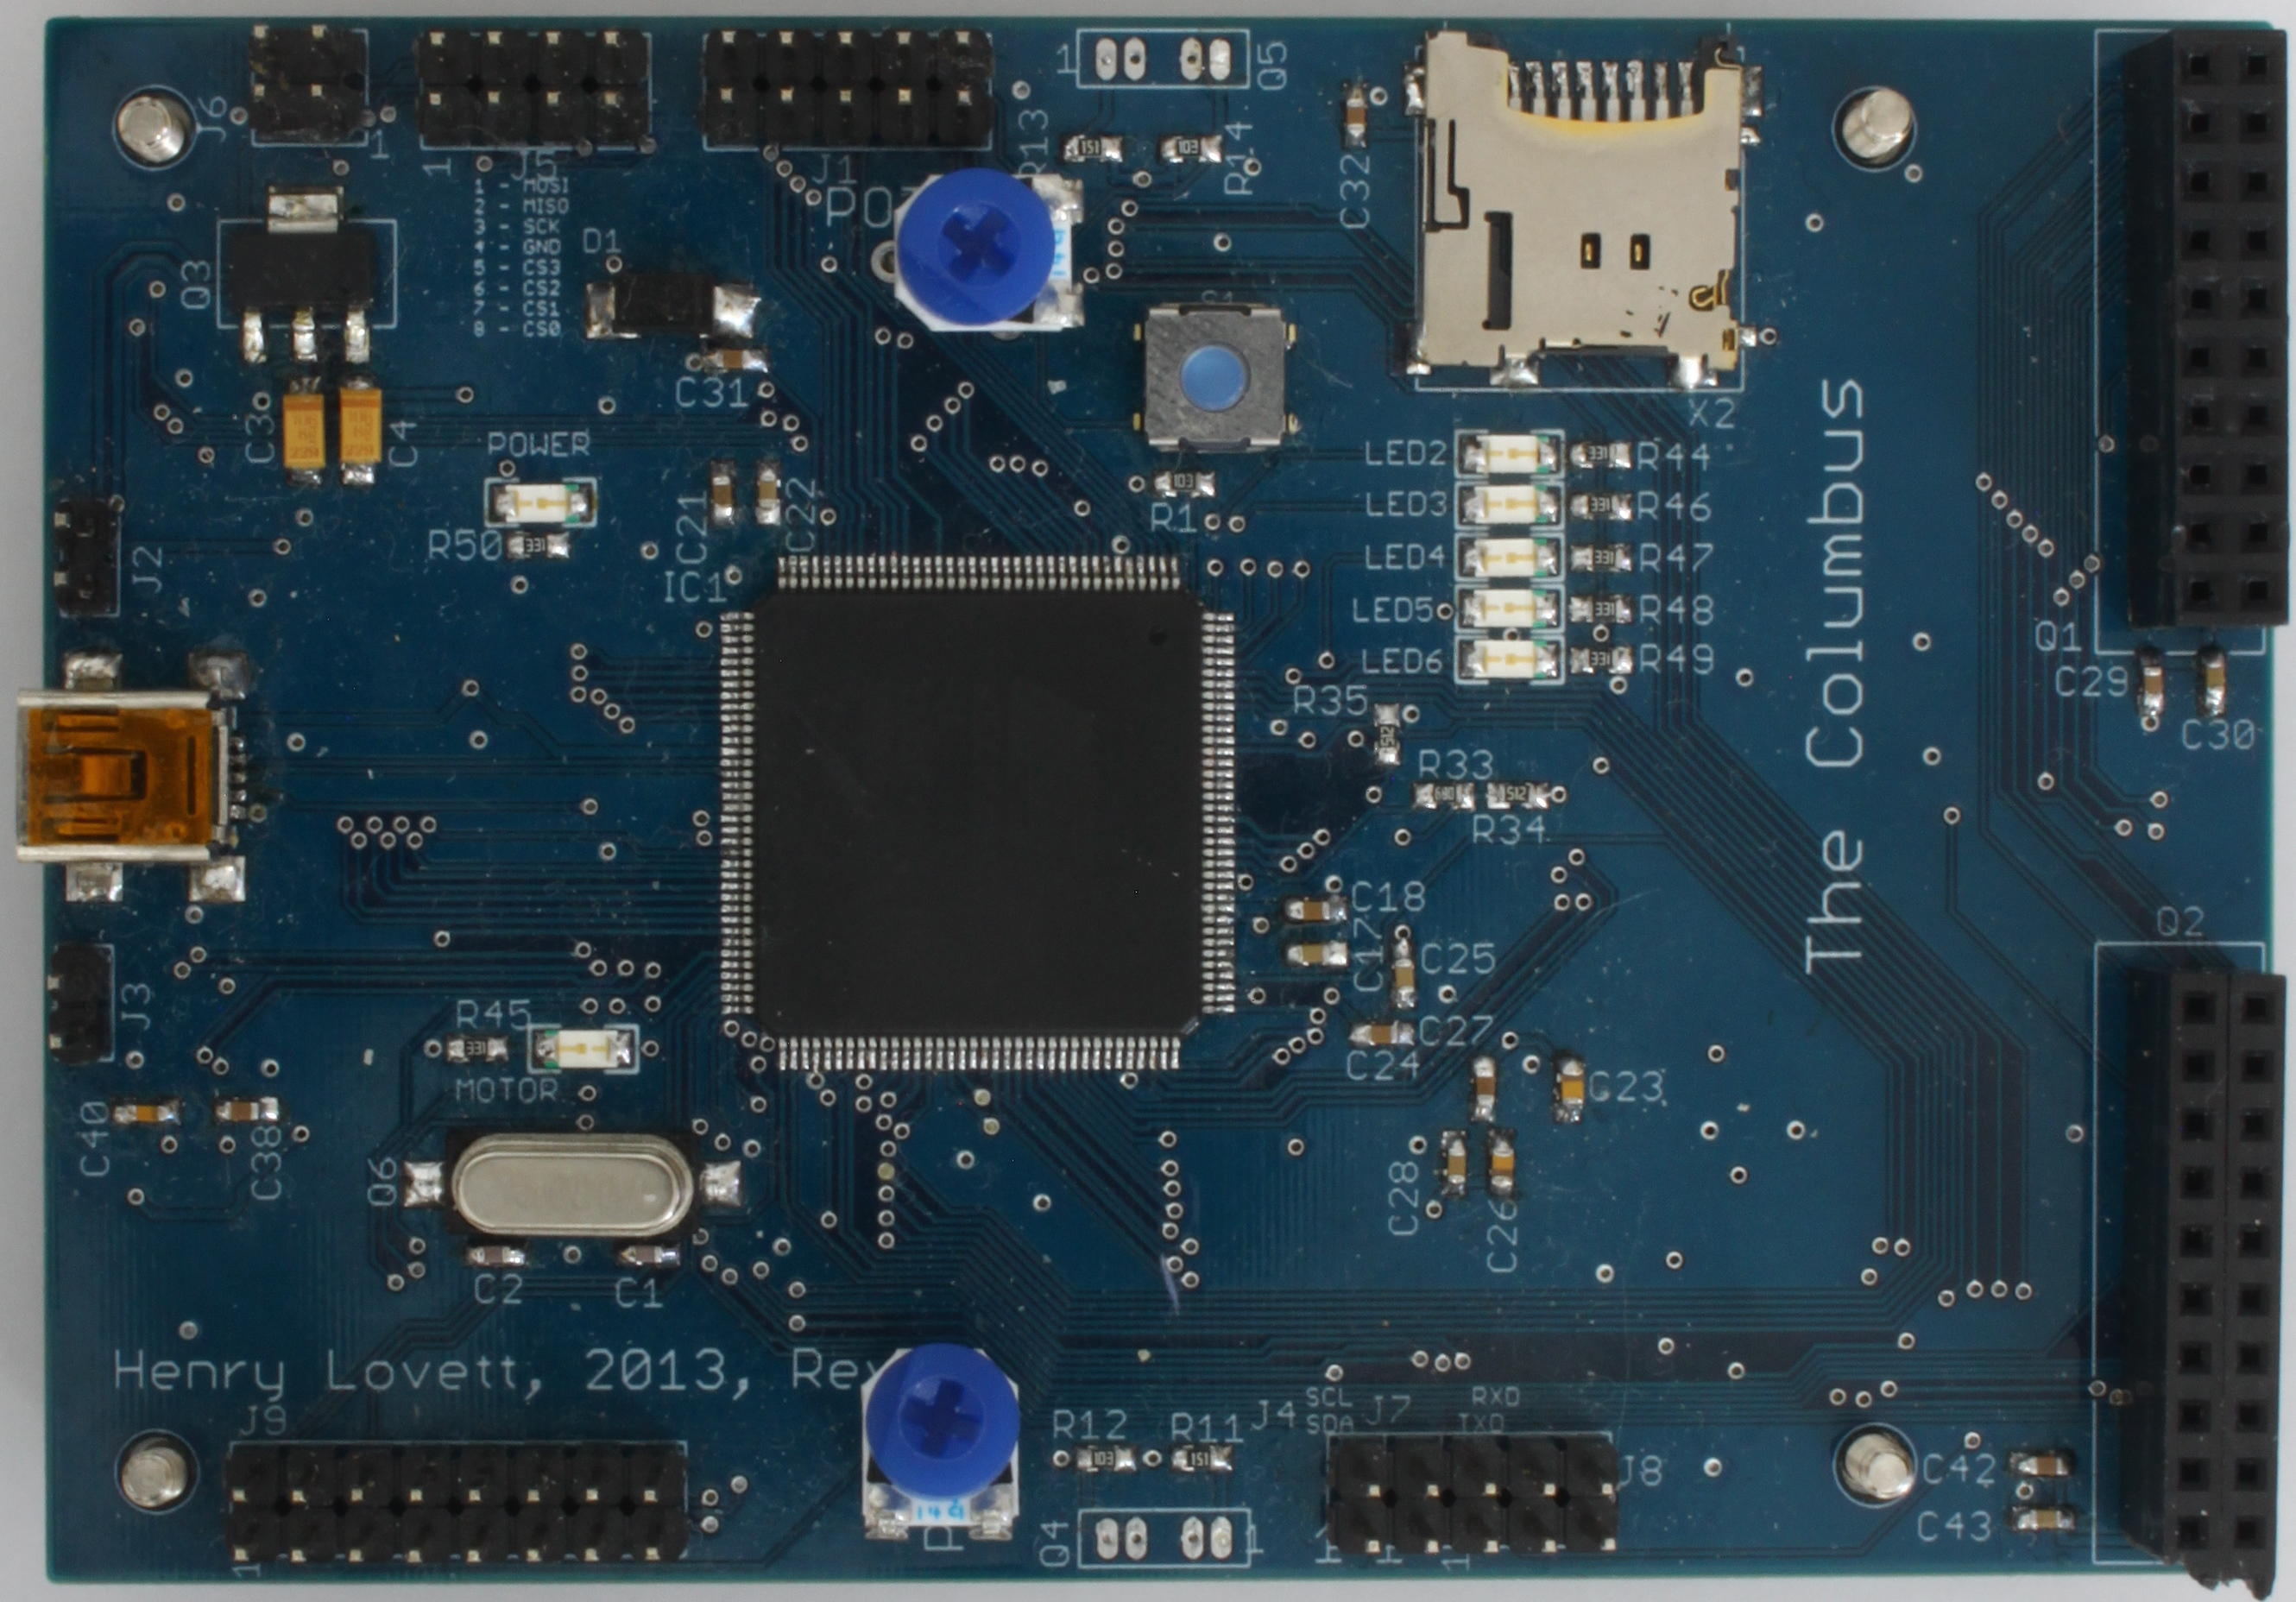
\includegraphics[width = \textwidth, keepaspectratio]{./Figures/PCB_Top.jpg} }
\subfigure[Bottom view of built PCB with SDRAM chip select patch \label{fig:PCB:Bottom}]{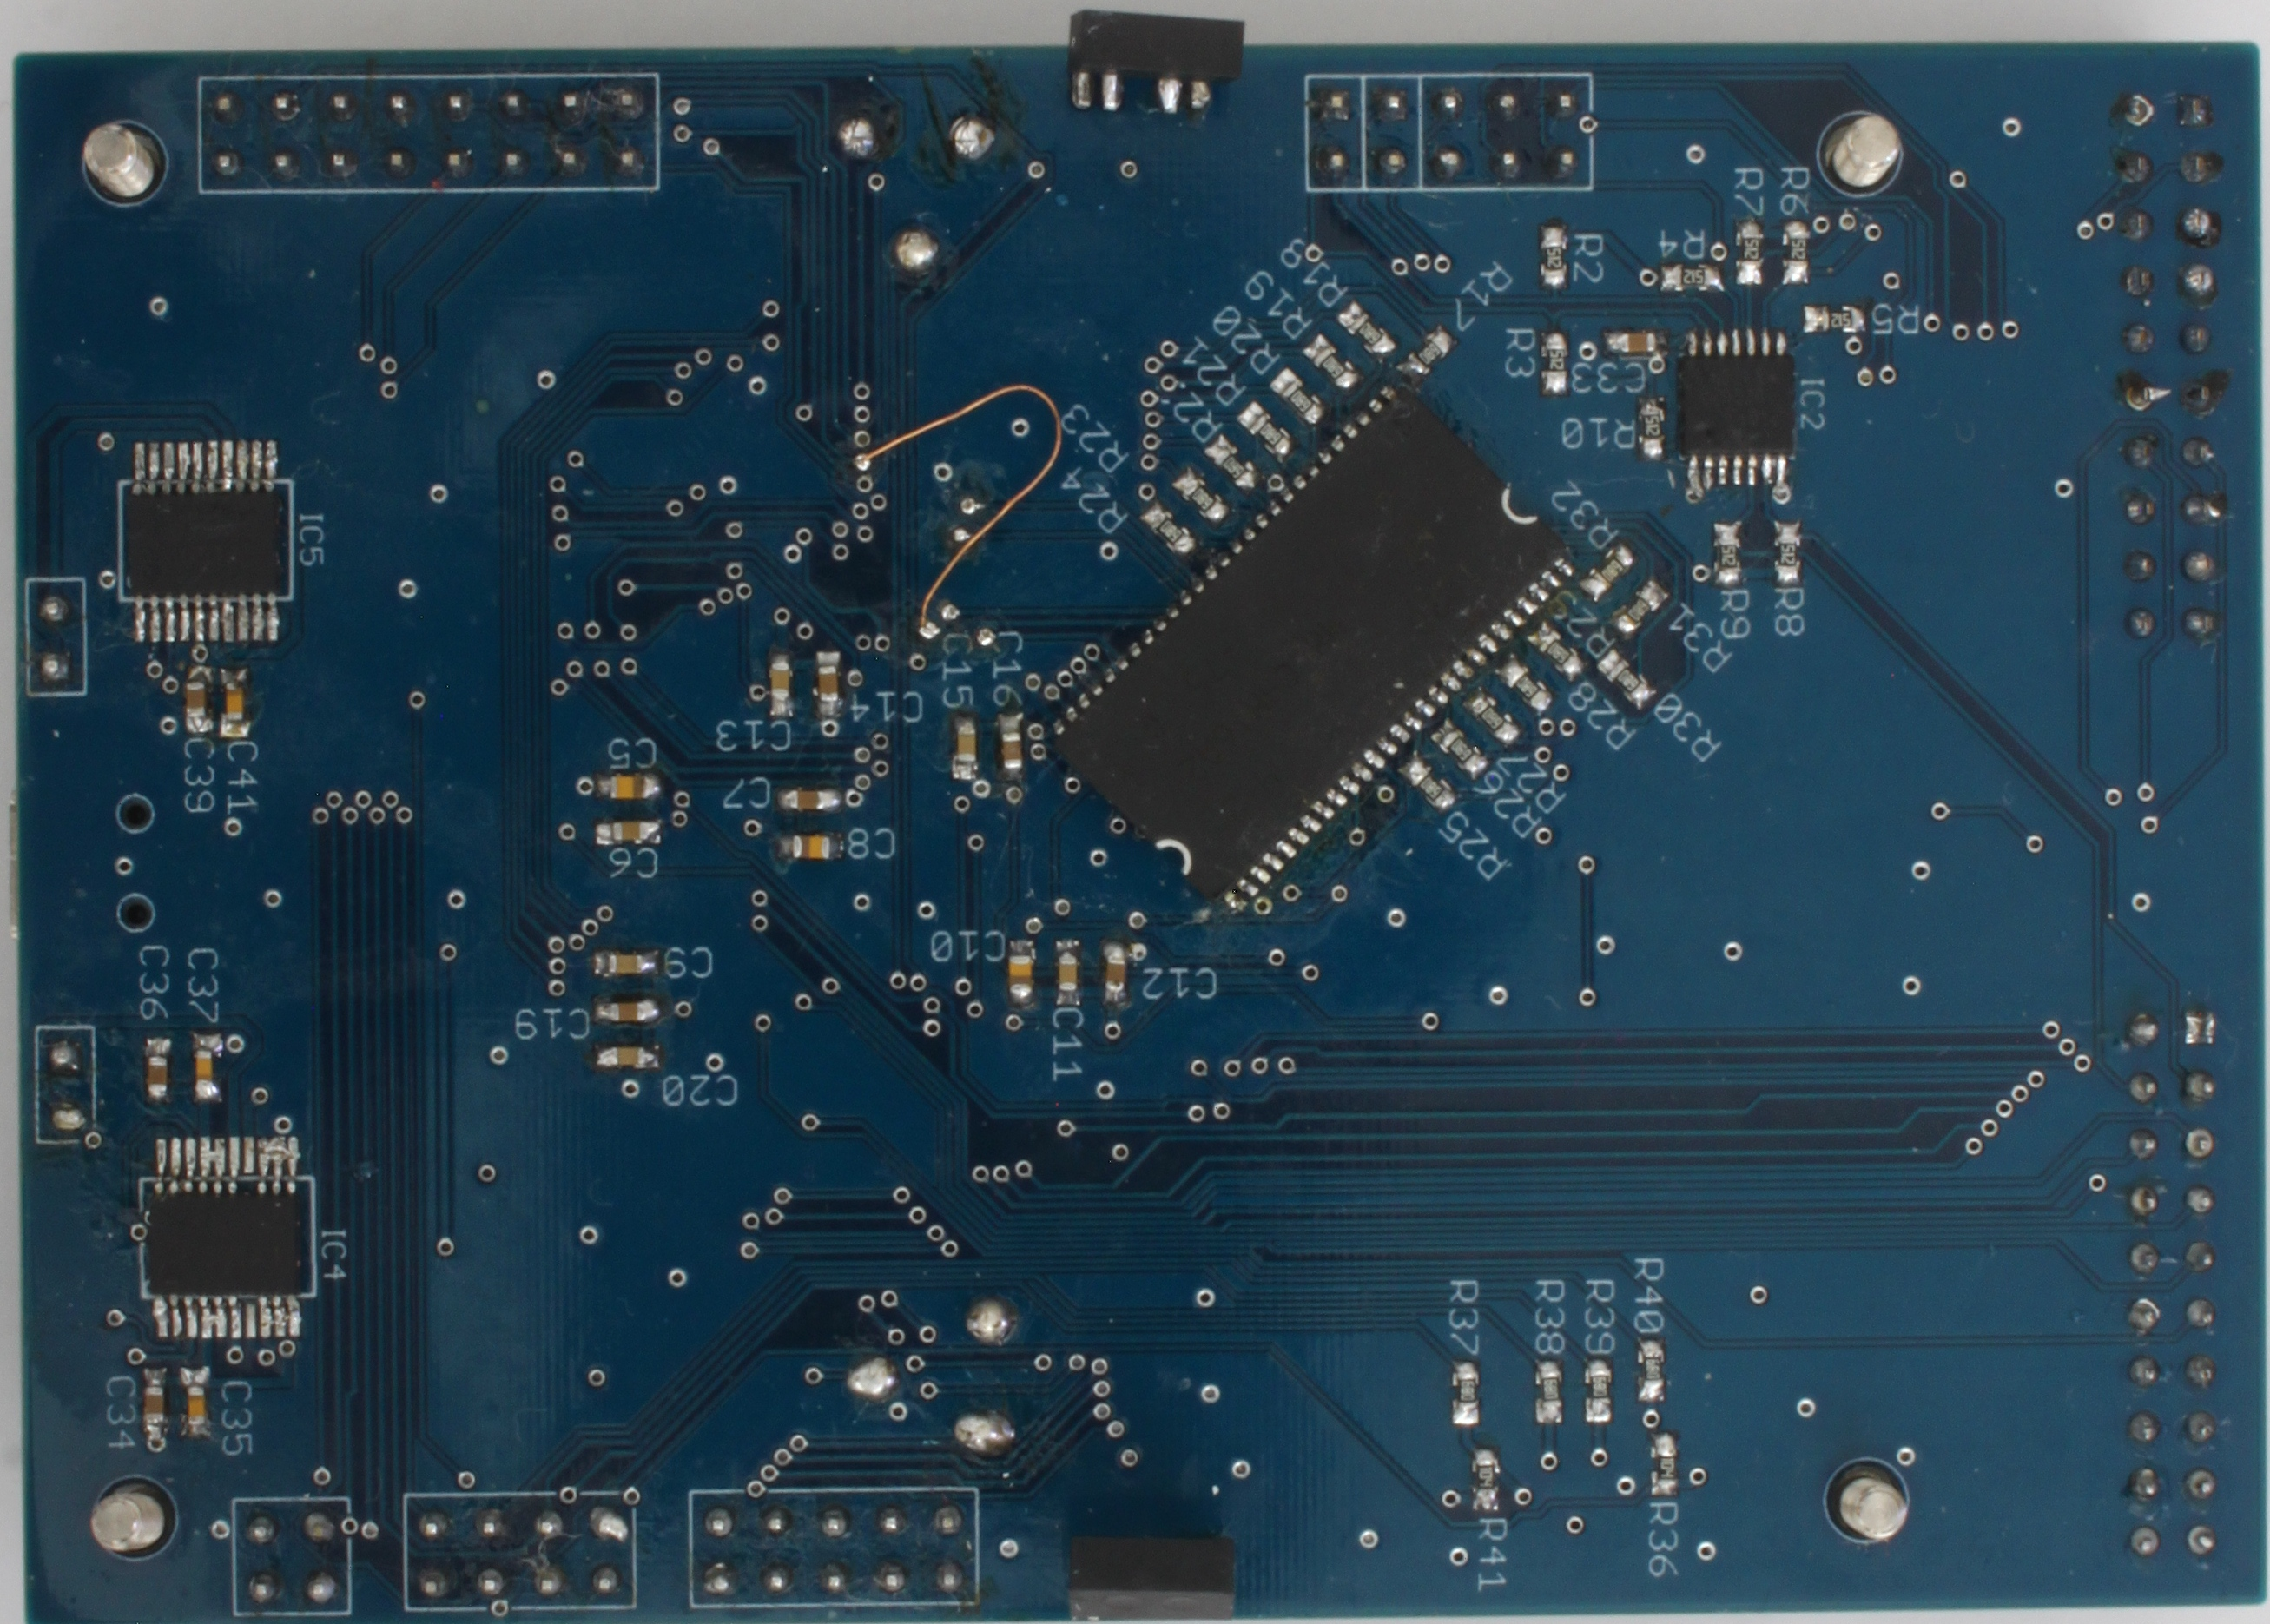
\includegraphics[width = \textwidth, keepaspectratio]{./Figures/PCB_Bottom.jpg} }
\caption{Pictures of the built PCB.}
\label{fig:PCB:Built}
\end{figure}

%% ----------------------------------------------------------------
%% InvestigationVision.tex
%% ---------------------------------------------------------------- 
\chapter{Vision Algorithms} \label{Chapter:InvestigationVision}

\section{Matching Algorithms}\label{Section:Comparison}
%\inote{find some references to back these claims up}
%\inote{Talk about how to compare images and TEST them all. Make a final comparison to decide on which will be used}
In computer vision, there are many different ways of comparing two similar images. These include the sum of absolute differences (SAD) \citep{Hamzah:DistanceDetection}, the sum of squared differences (SSD)\citep{Mrovlje:Distance_Stereoscopic} and  normalised cross correlation (NCC)\citep{zhao2006image}. Each of these methods will be explained and tested in order to compare them. All testing will use images seen in Figure \ref{fig:StereoTest}. Each test uses the same size template ($50px\times50px$) to compare the two images. 

\begin{figure}
\centering
\subfigure[Left Image]{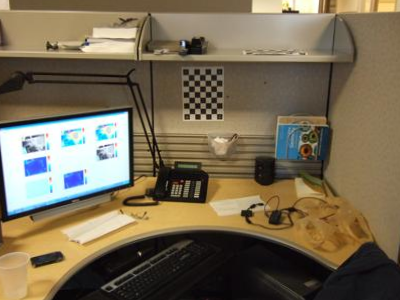
\includegraphics[scale=0.4]{./Figures/deskLeft.png} }
\subfigure[Right Image]{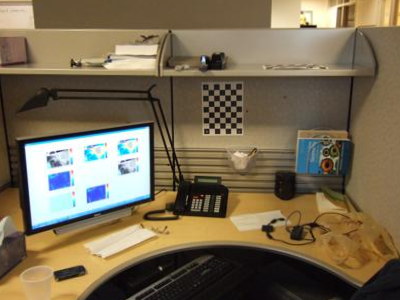
\includegraphics[scale=0.4]{./Figures/deskRight.png} }
\caption{Stereoscopic test images from MATLAB examples}
\label{fig:StereoTest}
\end{figure}


%Explanation of how they work
%\inote{Maybe do a basic 5x5 example for each?}
\subsection{Sum of Absolute Differences}\label{Section:SAD}

Given two identically sized two dimensional matrices, $A, B$, of dimensions $I,J$, SAD is defined as
\begin{equation} \label{eq:SAD}
SAD = \sum\limits_{i=0}^{I-1} \sum\limits_{j=0}^{J-1} A[i,j] - B[i,j] 
\end{equation}

This method subtracts the observed template from the expected. All differences are then added together. This algorithm is simple and requires a small amount of computation. The algorithm returns values where a small result means the two images are well matched.

\subsection{Sum of Squared Differences}\label{Section:SSD}
\begin{equation}\label{eq:SSD}
SSD = \sum\limits_{i=0}^{I-1} \sum\limits_{j=0}^{J-1} (A[i,j] - B[i,j] )^2
\end{equation}

This is very similar to SAD but adds more complexity by squaring each difference. This removes the ability of equally different but opposite differences cancelling each other out (grey to white of one pixel will cancel out a white to grey difference in another with SAD). Again, a low result is a match in this case.

%\inote{sort chi out, if I want to do it...}
%\subsection{'Chi Squared'}
%$\chi ^{2}$ is ``Insert definition here". For use with images the equation can be adapted to \ref{eq:ChiSquare}. 
%
%\begin{equation} \label{eq:ChiSquare}
%\chi ^{2} = \sum\limits_{i=0}^{I-1} \sum\limits_{j=0}^{J-1}\frac{(A[i,j] - B[i,j])^2}{(A[i,j]+B[i,j])/2}
%\end{equation}


\subsection{Normalised Cross Correlation}\label{Section:NCC}
\begin{equation}\label{eq:NCC}
NCC =  \frac{1}{n}\sum\limits_{i,j} \frac{(A[i,j] - \bar{A}).(B[i,j] - \bar{B})}{\sigma _A . \sigma _B}
\end{equation}
\begin{center}
Where $n$ is the number of pixels in $A$ and $B$, \\$\sigma$ is the standard deviation of the image, and \\$\bar{A}$ is the a average pixel value. 
%\inote{Find a source for this equation}
\end{center}
%\inote{No date on Reference}
NCC is very similar to cross correlation, but normalised to reduce the error if one image is brighter than the other. This is common in computer vision \citep{Tsai:NCC} and cross correlation is often used in digital signal processing, so fast algorithms have been made to calculate this. 

Unlike SSD and SAD, the normalised cross correlation gives a high value for a match. The downside to this algorithm comes with the complexity of the equation as it contains division and the calculation of the square root of a number in order to find the standard deviation. 
Floating point arithmetic is extensively used, which takes much more time to execute on a microcontroller than pure integer arithmetic.
%These operations are rarely implemented in hardware and are time consuming to carry out in software. They also require floating point registers and operates slowly on a microcontroller without any. 



%test and compare
\subsection{Comparison}

To compare these equations, a $50px \times 50px$ template taken from the right picture was compared with the left image over the entire valid range. The coordinates on the graph give the centre pixel of the calculation. 

\begin{figure}
\centering
\subfigure[S.A.D results - blue shows areas of matching\label{fg:Results:SAD}]{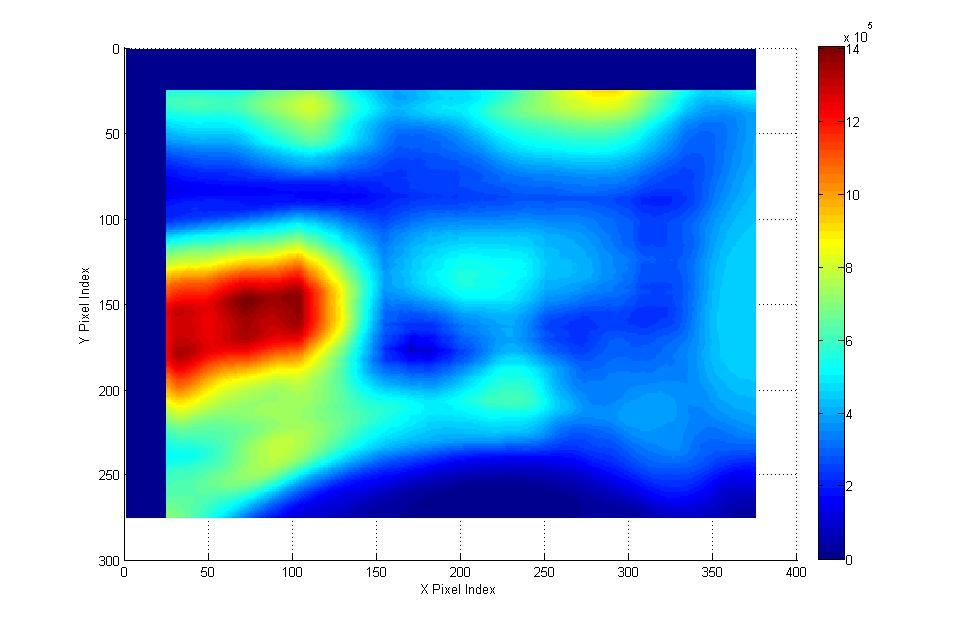
\includegraphics[width = 12cm, keepaspectratio]{./Figures/SADResults.eps} }
\subfigure[S.S.D. results - blue shows areas of matching\label{fg:Results:SSD}]{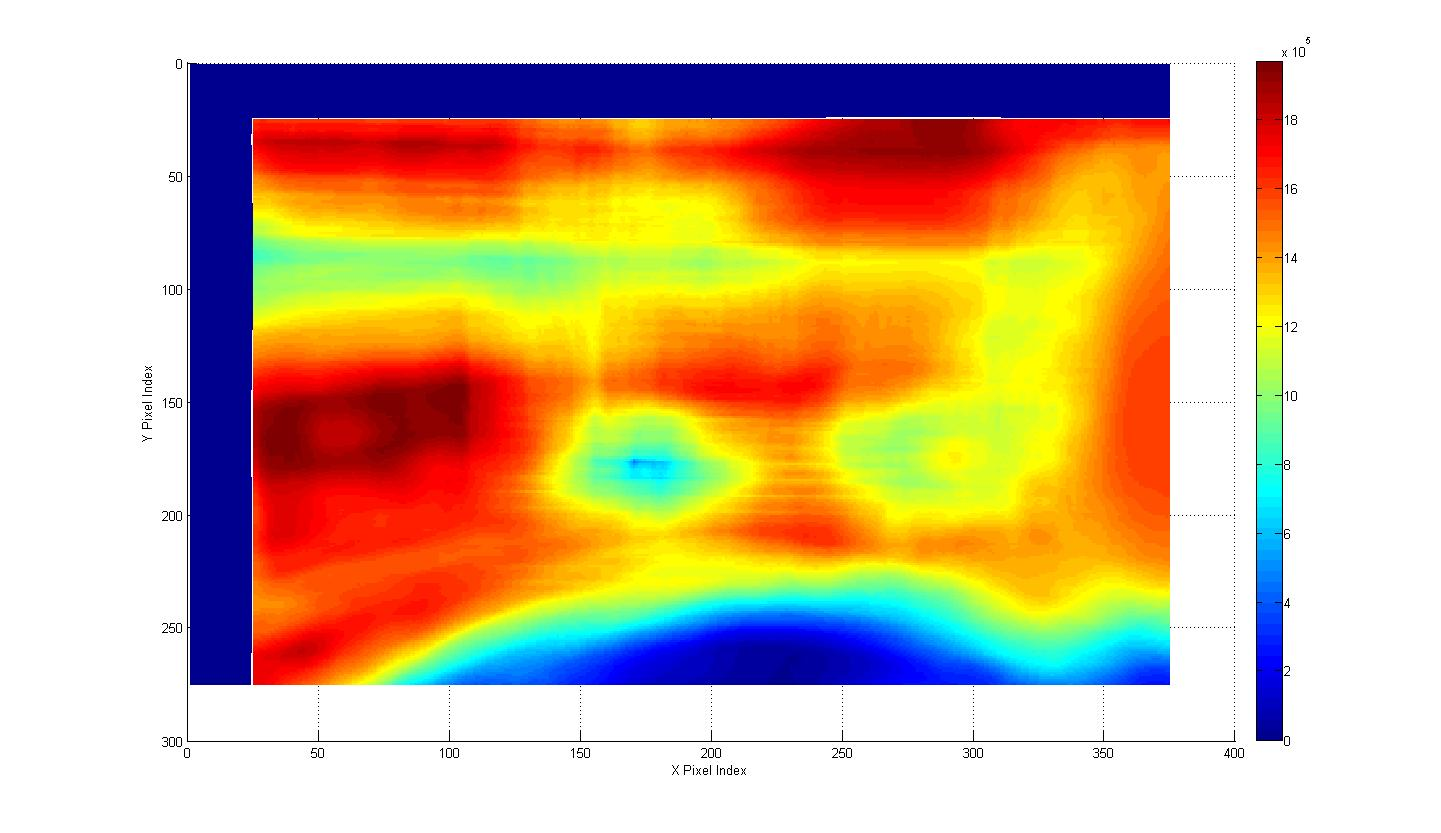
\includegraphics[width = 12cm, keepaspectratio]{./Figures/SSDResults.eps} }
\subfigure[N.C.C. results - red shows areas of matching\label{fg:Results:NCC}]{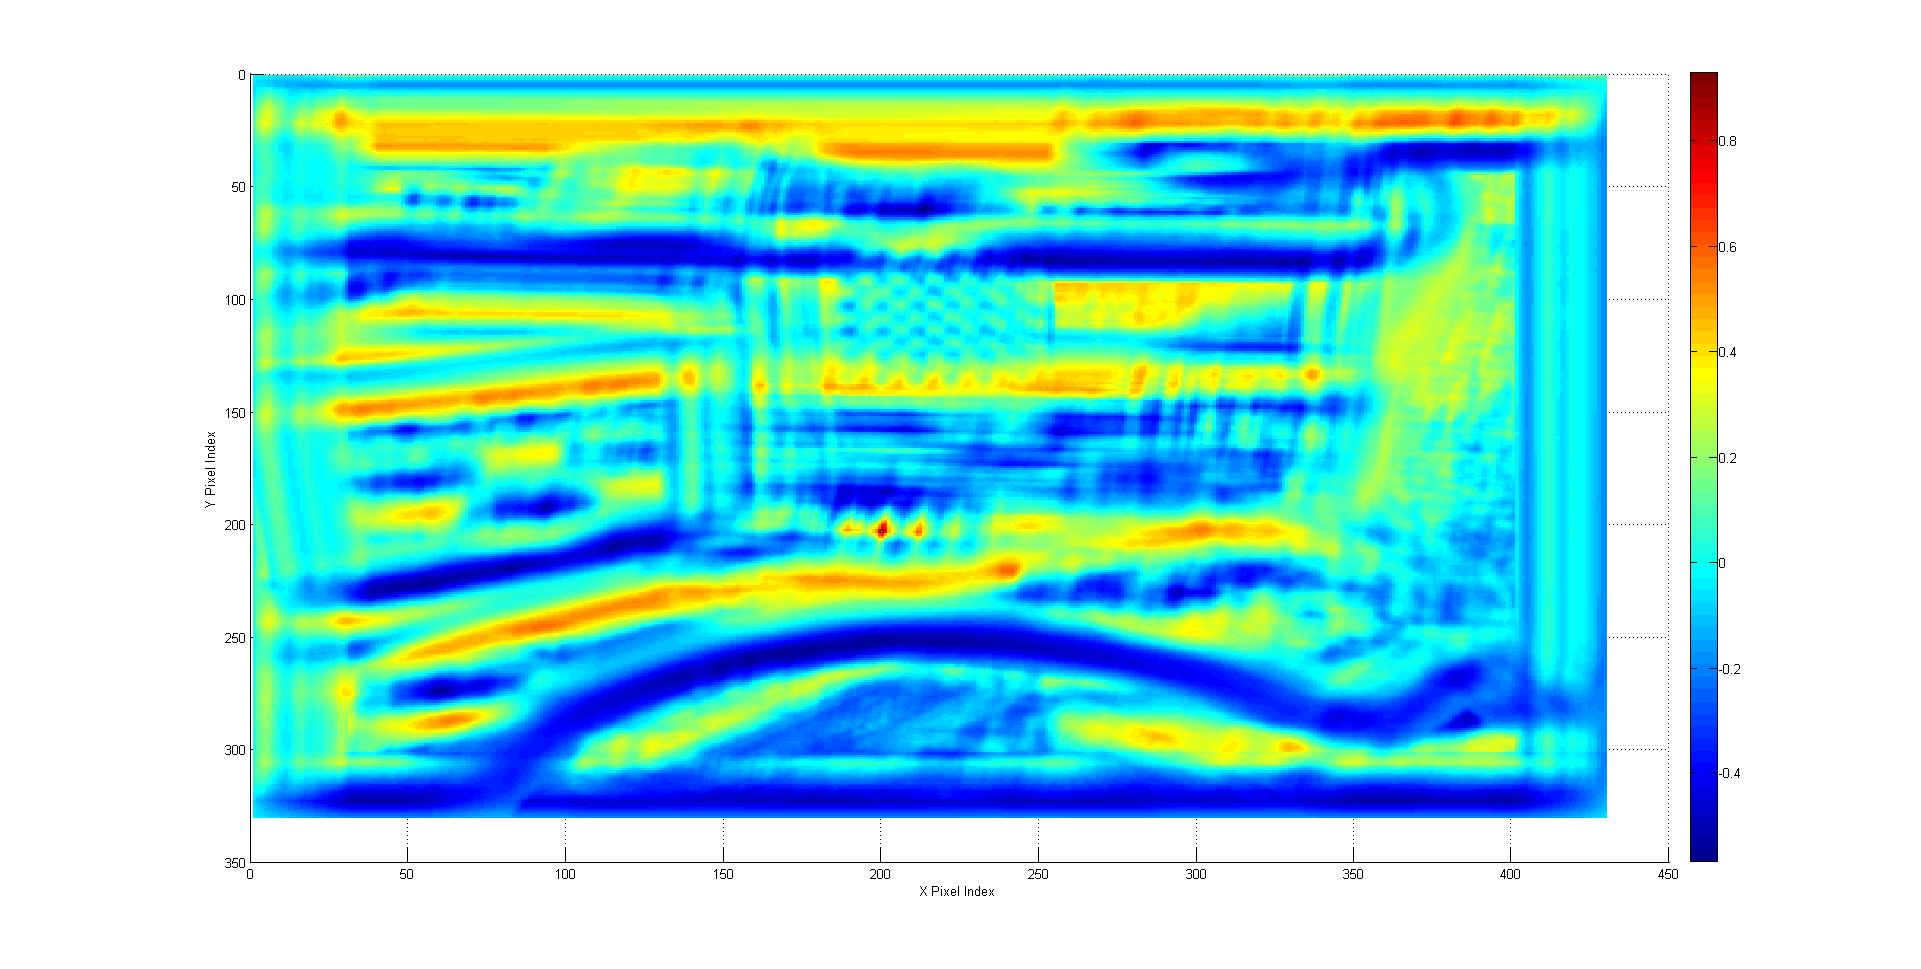
\includegraphics[width = 12cm, keepaspectratio]{./Figures/NCCResults.eps} }
\caption{Result graphs of comparison algorithms}
\label{fg:CompResults}
\end{figure}

Each graph shows the correct area being identified as a match, but this also highlights the downfalls of the SAD and SSD methods. The graphs in Figure \ref{fg:CompResults} are rotated to match the orientation of the images in Figure \ref{fig:StereoTest}. Each of the images is tested by attempting to match the desk phone from the right image to the entirety of the left image. The actual match should be around $(170, 176)$. An exact result cannot be estimated as the images are not matched perfectly - there isn't an exact integer of pixel difference between the images. This is the sub pixel problem \citep{haller2012design}.

SAD results in Figure \ref{fg:Results:SAD} show large areas of matching. A minimum occurs around the location expected($170,175$) of a value of $5.66\times 10^4$. 
However, the dark area beneath the desk is a false detection. The SAD algorithm detects a greater comparison with a low value of $3370$ at $(227, 275)$ which causes a false match.
%However, along the bottom of the image, where a dark area occurs below the desk in the lower part of figures \ref{fig:StereoTest}, the SAD algorithm detects a greater comparison, with the lowest value in this area being $3370$ at $(227, 275)$. This creates a false detection here. 

SSD, Figure \ref{fg:Results:SSD}, shows matches in the same two areas: where a match should occur and the dark area beneath the desk. The minimum value where the match should occur is $4.355 \times 10^5$ at location $(170,176)$. However, there is a large match correlation between the dark area under the desk where the actual lowest value of $2.768\times10^4$ occurs at $(225,274)$. This, again, is a false match and is a downfall of this algorithm.

The NCC results are visible in Figure \ref{fg:Results:NCC}. A match can be seen at coordinate $(195,201)$ with a peak value of $0.9654$. The coordinate is different to the previous results because the cross correlation works over the boundary of the image creating more results. The dimensions of the image are $300px \times 400px$, but the NCC returns a dataset of dimensions $350px \times 450px$ when using a template size of $50px\times 50px$. To get the actual match, half of the box size must be subtracted from the returned coordinate. This means the match occurs at $(170,176)$. With this algorithm, there is no area of the image which is close to a false detection. 

\subsection{Conclusion}
It is apparent that there is a direct correlation between the complexity of the matching algorithm to the reliability of the match returned. In brightly lit, colourful environments absent of dark colours, SAD and SSD should provide a reliable result, but this cannot be guaranteed to always be the case. Therefore further development of the matching algorithm will start with using the normalised cross correlation. A comprise between complexity and reliability needs to be reached, where reliability is the more desirable of the two. Cross correlation is also widely used in digital signal processing, so optimised algorithms suitable for microcontrollers do exist.

\section{Range Finding}
\subsection{Derivations}

By using two images separated by a horizontal distance, $B$, the range of an object can be found given some characteristics of the camera. Appendix \ref{Appendix:Range} contains the derivations for the follow scenarios:

\begin{enumerate}
\item Object is between the cameras (Figure \ref{problem_between})
\item Object is in left or right hand sides of both images (Figure \ref{problem_toleft})
\item Object is directly in front of a camera (Figure \ref{fig:problem_infront})
\end{enumerate}


\subsection{Summary}
There are three situations that can occur. These are listed below with their equations.

Object is between the two cameras:
\begin{equation} \label{eq:summary:1}
D = \frac{Bx_0}{2\tan(\frac{\varphi_0}{2})(x_1 - x_2)}
\end{equation}

Object is to the same side in both images:
\begin{equation} \label{eq:summary:2}
D = B.\frac{\cos(\varphi_2).\cos(\varphi_1)}{sin(\varphi_2 - \varphi_1)}
\end{equation}
Object is directly in front of a camera:
\begin{equation} \label{eq:summary:3}
D = B \tan\left(\frac{\pi}{2} - \varphi_{2}\right)
\end{equation}

Where $\varphi_1$ is defined in Equation \eqref{eq:p2:phi1} and $\varphi_2$ is defined in Equation \eqref{eq:p2:phi2}.
\begin{equation} \label{eq:p2:phi1}
\varphi_1 = \arctan\left(\frac{2x_1}{x_0}\tan\left(\frac{\varphi_0}{2}\right)\right)
\end{equation}
\begin{equation} \label{eq:p2:phi2}
\varphi_2 = \arctan\left(\frac{2x_2}{x_0}\tan\left(\frac{\varphi_0}{2}\right)\right)
\end{equation}
\\
When the images have been matched, these equations can be used to calculate the distance to an object.

\subsection{Field of View}
%The field of view is an important characteristic to calculate distances and must be measured for the camera. 
The field of view of the camera is an important variable that must be measured. Field of view was measured by placing a ruler at a distance in front of the camera and measuring the total distance seen across the image. Equation \eqref{eq:FoV}, derived from the set-up in Figure \ref{fig:FoV}, was then used to calculate the field of view. This was done multiple times for accuracy. Results can be seen in Table \ref{table:fieldofview}. The field of view used is the average of the data set and was found to be $\varphi_0 = 0.6249^c$. 
\begin{figure}
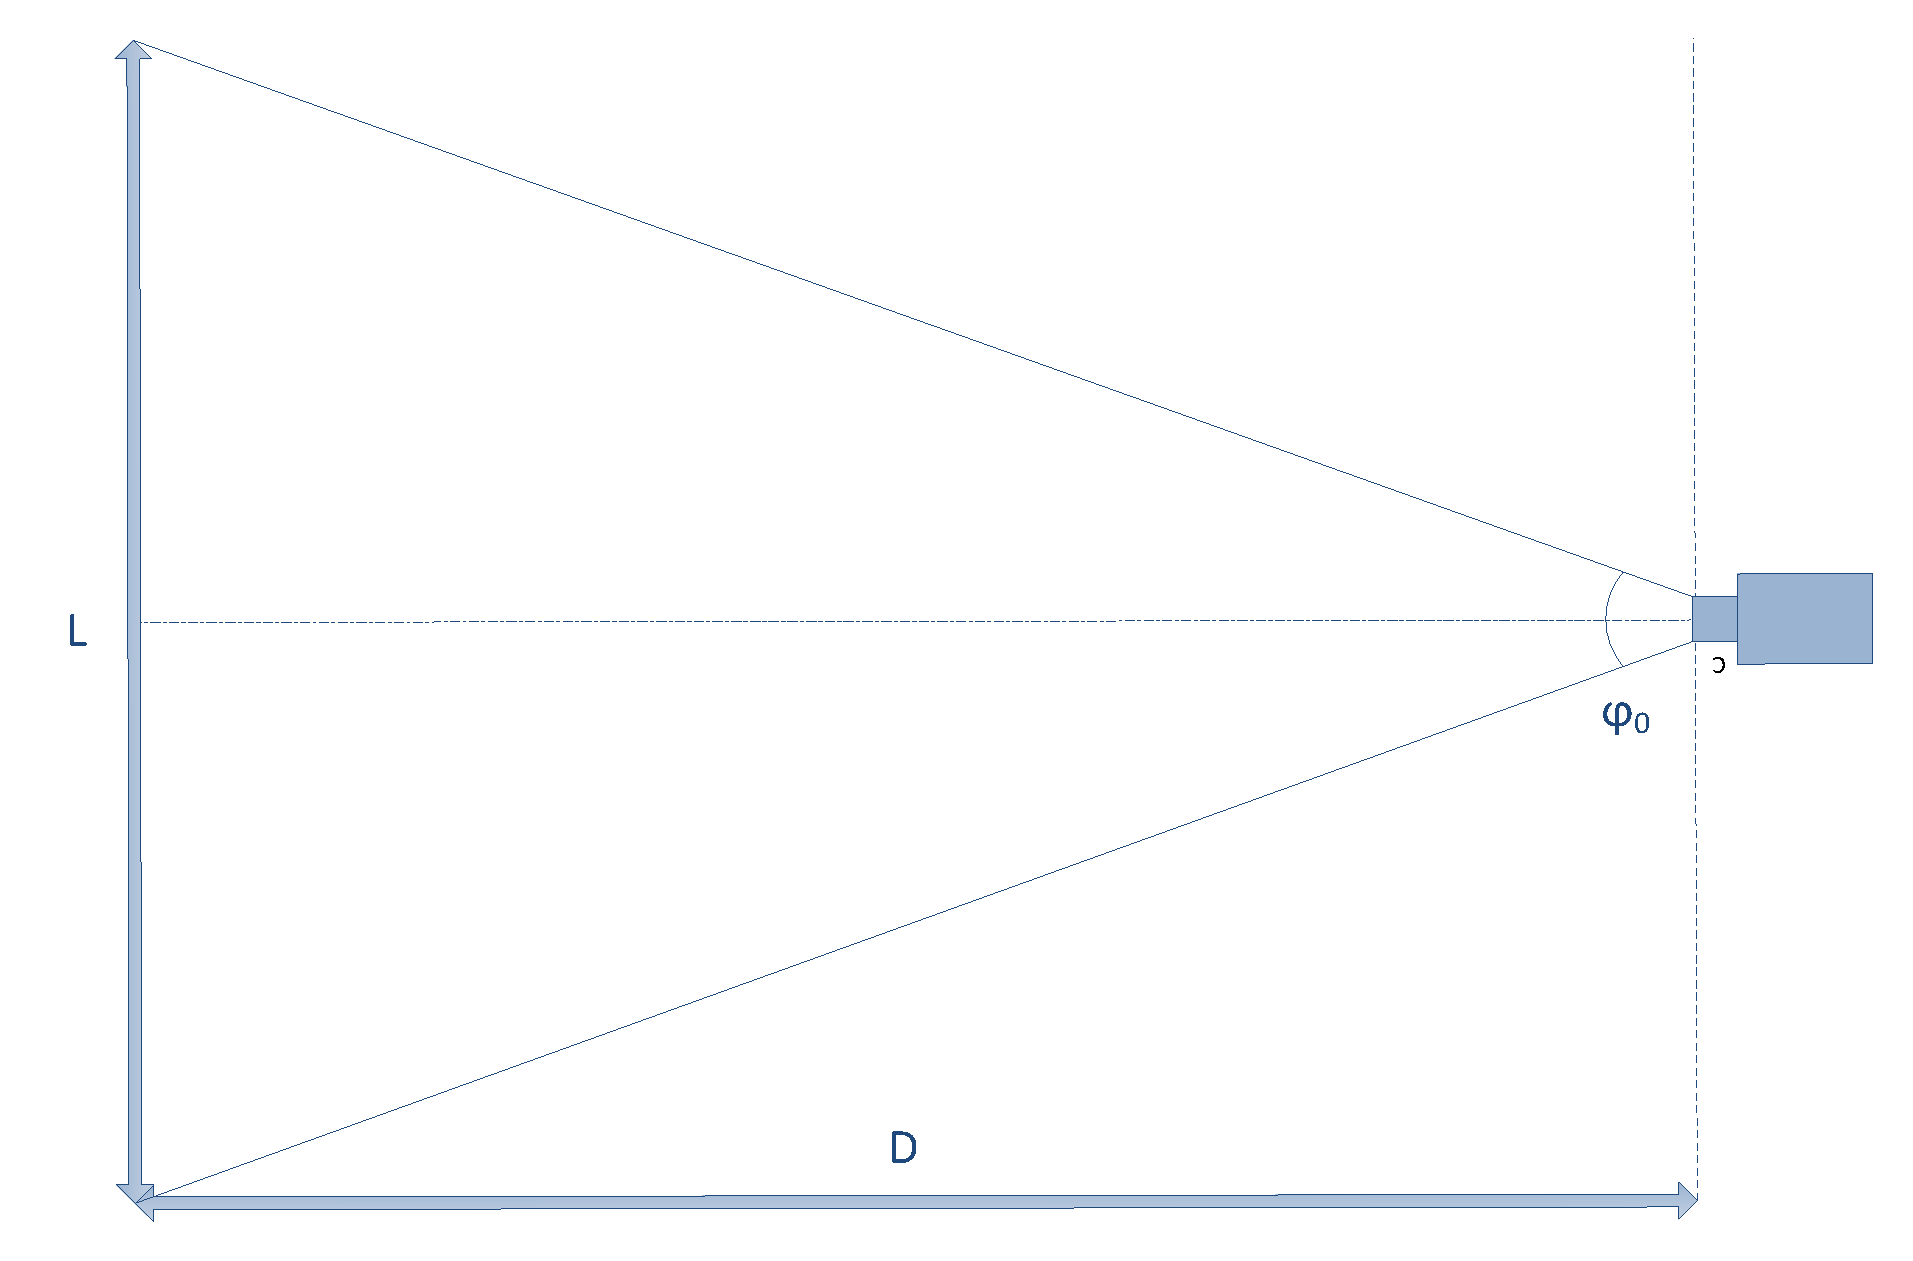
\includegraphics[width=\textwidth]{Figures/FoV.pdf}
\caption{Diagram of the set-up to measure the field of view of the camera}
\label{fig:FoV}
\end{figure}
\begin{equation}\label{eq:FoV}
\varphi_0 = 2\arctan\left(\frac{L}{2D}\right)
\end{equation}
\begin{table}
\caption{Table of results to calculate the field of view of the camera}
\label{table:fieldofview}
\centering
\begin{tabular}{ccc} \toprule
\textbf{L (mm)} & \textbf{D (mm)} &$\boldsymbol{\varphi (^c)}$ \\ \toprule
70 & 104 & 0.6435\\\midrule
90 & 135 &0.6015\\\midrule
178 & 285 &0.6054\\ \midrule
214 & 345 &0.6493 \\ \bottomrule
\multicolumn{2}{c}{Average} & 0.6249 \\ \bottomrule
\end{tabular}

\end{table}



\subsection{Testing}
MATLAB was used to test the range finding. It is unable to automatically detect an object so the user must select the template when prompted. 

A stereo pair of images of a rubber duck at different ranges were captured using the completed robot. To calculate the distance, a template from the right image of the duck's head was cross correlated with the left image. The maximum peak in the result was found and used as the match point. The distance was then calculated using Equation \eqref{eq:summary:1}, with $B=42mm$, $\varphi_0=0.6249$ and $x_0=320$. Example images can be seen in Figure \ref{fig:duck:stereo} and an example NCC result can be seen in Figure \ref{fig:duck:ncc}. 

Table \ref{table:range} shows the distances tested with the distance calculated using the above method. The ranges calculated were inaccurate. Matching can only be achieved to the accuracy of a few pixels without a more complex design, and therefore can introduce a small error when matching and cause a large distance error in the calculation. 

\begin{table}
\centering
\caption{Results of range finding test}
\label{table:range}
\begin{tabular}{p{3cm}p{3cm}p{3cm}p{3cm}} \toprule
\textbf{Actual Distance (mm)} & \textbf{Pixel Difference in Images (pixel)} & \textbf{Calculated Distance (mm)} & \textbf{Error (\%)} \\ \toprule
100 & 290 & 72 & 28\\ \midrule
200 & 152 & 137 & 32\\ \midrule
300 & 109 & 191 & 36\\ \midrule
400 & 88 & 236 & 41\\ \midrule
500 & 75 & 277 & 45\\ \midrule
600 & 67 & 310 & 48\\ \midrule
700 & 61 & 341 & 51\\ \midrule
800 & 57 & 365 & 54\\ \midrule
900 & 53 & 393 & 56\\ \midrule
1000 & 51 & 408 & 59\\ \bottomrule
\end{tabular}
\end{table}
\begin{figure}
\centering
\subfigure[Left image]{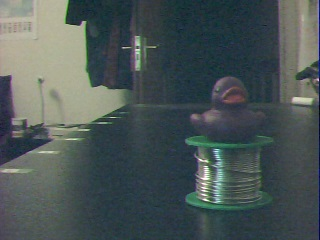
\includegraphics[scale=0.4]{./Figures/Duck_L.jpg} }
\subfigure[Right image]{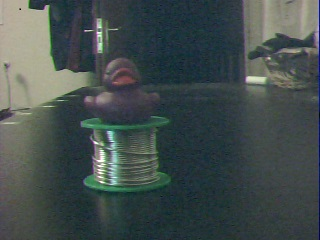
\includegraphics[scale=0.4]{./Figures/Duck_R.jpg} }
\caption{Stereo pair of images of a rubber duck on a reel of solder}
\label{fig:duck:stereo}
\end{figure}


\begin{figure}
\includegraphics[width=\textwidth]{Figures/NCC_Duck.eps}
\caption{NCC results from matching using the duck's head from the right image as the template to the left image}
\label{fig:duck:ncc}
\end{figure}


\subsection{The Effect of Resolution and Field of View}

By simplifying Equation \eqref{eq:summary:1} to \eqref{eq:range:simp} shows that the function is at a maximum when $\Delta_x = 1$ and is the maximum distance able to be calculated. The maximum error is found using Equation \eqref{eq:range:maxerr} and shows that the error increases with resolution. 

\begin{equation}\label{eq:range:simp}
D(\Delta_x) = \frac{B.x_0}{2\tan \left(\frac{\varphi_0}{2}\right).\Delta_x}
\end{equation}

\begin{equation}\label{eq:range:maxerr}
Err_{max} = D(1) - D(2) = \frac{B.x_0}{2\tan \left(\frac{\varphi_0}{2}\right)} - \frac{B.x_0}{2\tan \left(\frac{\varphi_0}{2}\right).2} = \frac{B.x_0}{4\tan \left(\frac{\varphi_0}{2}\right)}
\end{equation}

This is because as $x_0$ increases, the range of $(x_1 - x_2)$ also increases. The minimum detectable distance, Equation \eqref{eq:range:min}, is not related to resolution, but depends on $B$ and $\varphi_0$. 

\begin{equation}\label{eq:range:min}
D(x_0) = \frac{B}{2\tan \left(\frac{\varphi_0}{2}\right)}
\end{equation}

Figure \ref{fig:MaxR} shows the relationship between maximum distance, $x_0$ and $\varphi_0$. By increasing the horizontal resolution, the maximum distance increases, but also increases the error. Increasing $\varphi_0$ will lower the maximum distance, but the error will decrease and can be seen in Figure \ref{fig:DeltaxPhi0}. A compromise must be made between maximum distance and resolution. 

\begin{figure}
\includegraphics[width=\textwidth]{Figures/Distance_Phi0_X0.eps}
\caption{A surface plot of the maximum range able to be found with varying $\varphi_0$ and $x_0$. $B=42mm$, $\Delta_x = 1$}
\label{fig:MaxR}
\end{figure}
\begin{figure}
\includegraphics[width=\textwidth]{Figures/DeltaXPhi0.eps}
\caption{A surface plot of the range of distances able to be calculated with a range of field of views. $B=42mm$, $x_0 = 320$.}
\label{fig:DeltaxPhi0}
\end{figure}

\subsection{Conclusion}

Extensive testing of the effect of separation has been done before \citep{Mrovlje:Distance_Stereoscopic}. Figure \ref{fig:B:Plot} shows that increasing B will give you a larger range of detectable distances, but with a larger maximum error. Resolution also increases the error and maximum detectable distance. In reality, cameras have not increased only by resolution, but the lens have become wider angled as well. 

In order to improve the ability of these cameras for range finding, adding a wide angle lens will reduce the error at the expense of reducing the maximum range. Alternatively, the robot could use an algorithm to view the object at different perspectives to estimate the distance to it. 

The robot was designed to be small, and the cameras were chosen as a cheap alternative to more expensive products on the market. The test results show that by using cameras as described, ranges cannot accurately be measured. The separation of objects in the images is a reciprocal function and the data gathered in the test matches this characteristic, see Figure \ref{fig:Distance:DeltaX}. This means the system can perceive depth from the separation of the objects, but not accurately calculate the distance. 

\begin{figure}
\includegraphics[width=\textwidth]{Figures/BPlot.eps}
\caption{3D surface plot graph showing range of distances that can be calculated over a range of camera separation, B, values}
\label{fig:B:Plot}
\end{figure}
\begin{figure}
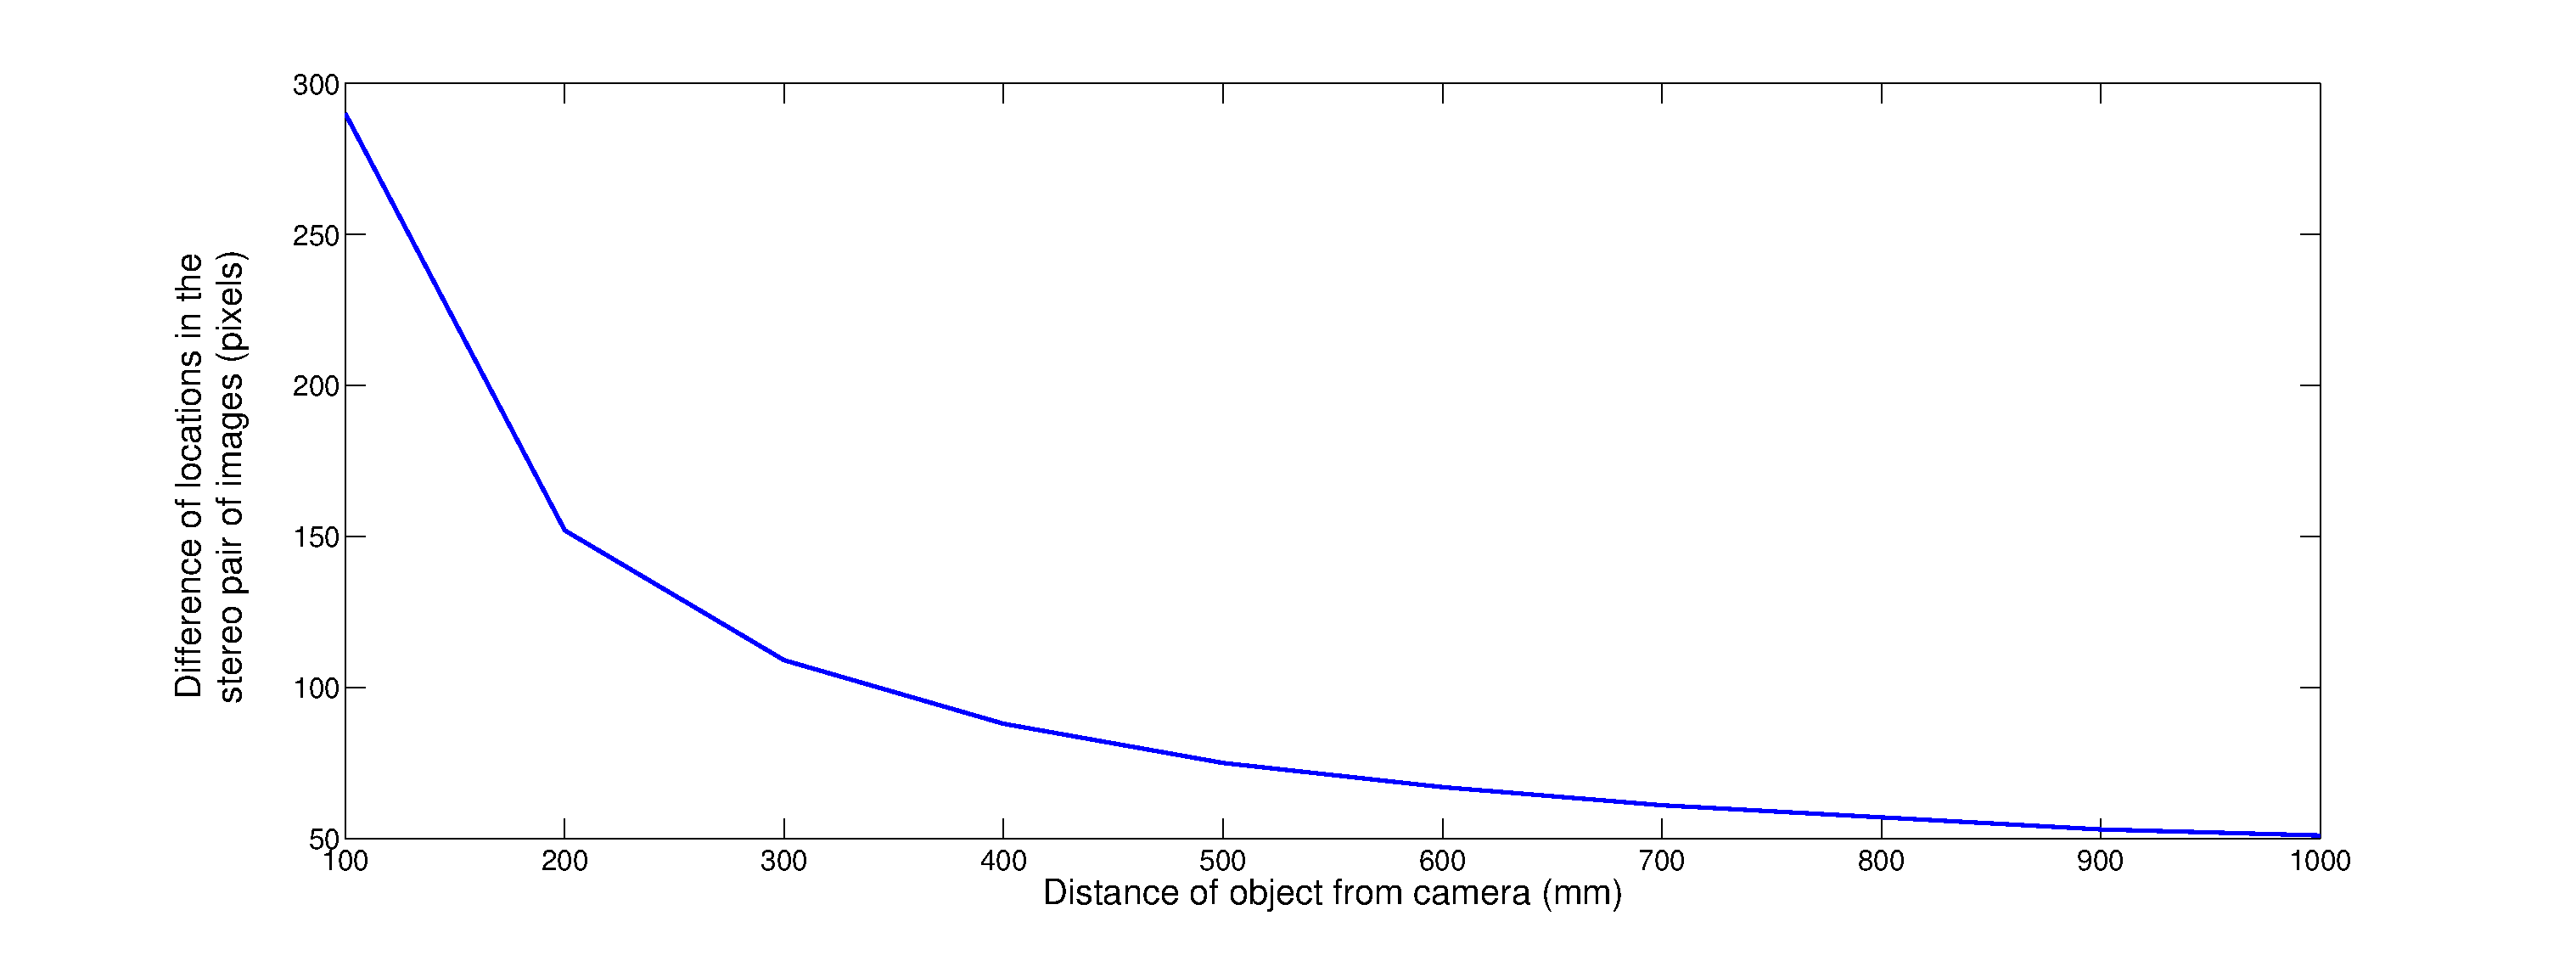
\includegraphics[width=\textwidth]{Figures/Distance_DeltaX.eps}
\caption{Graph showing distance of the object against the difference in the match locations}
\label{fig:Distance:DeltaX}
\end{figure}
\section{Fourier Transform}
\subsection{Background Research and the FFT}
The Fourier transform is a common tool in signal processing used for filer design, system analysis and image processing, as well as other applications. It transforms a time-based signal to the frequency domain, showing the frequency components contained in the signal as a complex number. This is often displayed as magnitude and phase. The Fourier transform is defined in Equation \eqref{eq:fourier} and two examples of signals and their Fourier transforms are shown in Figures \ref{fig:DiracFunctionFT} and \ref{fig:SquareWaveFT}. 
 
\begin{equation}\label{eq:fourier}
X(f) = \int\limits_{-\infty}^{\infty}x(t)e^{-\jmath 2 \pi ft}dt
\end{equation}

\begin{figure}
\centering
\subfigure[A graph showing a Dirac function\label{fg:Dirac:Signal}]{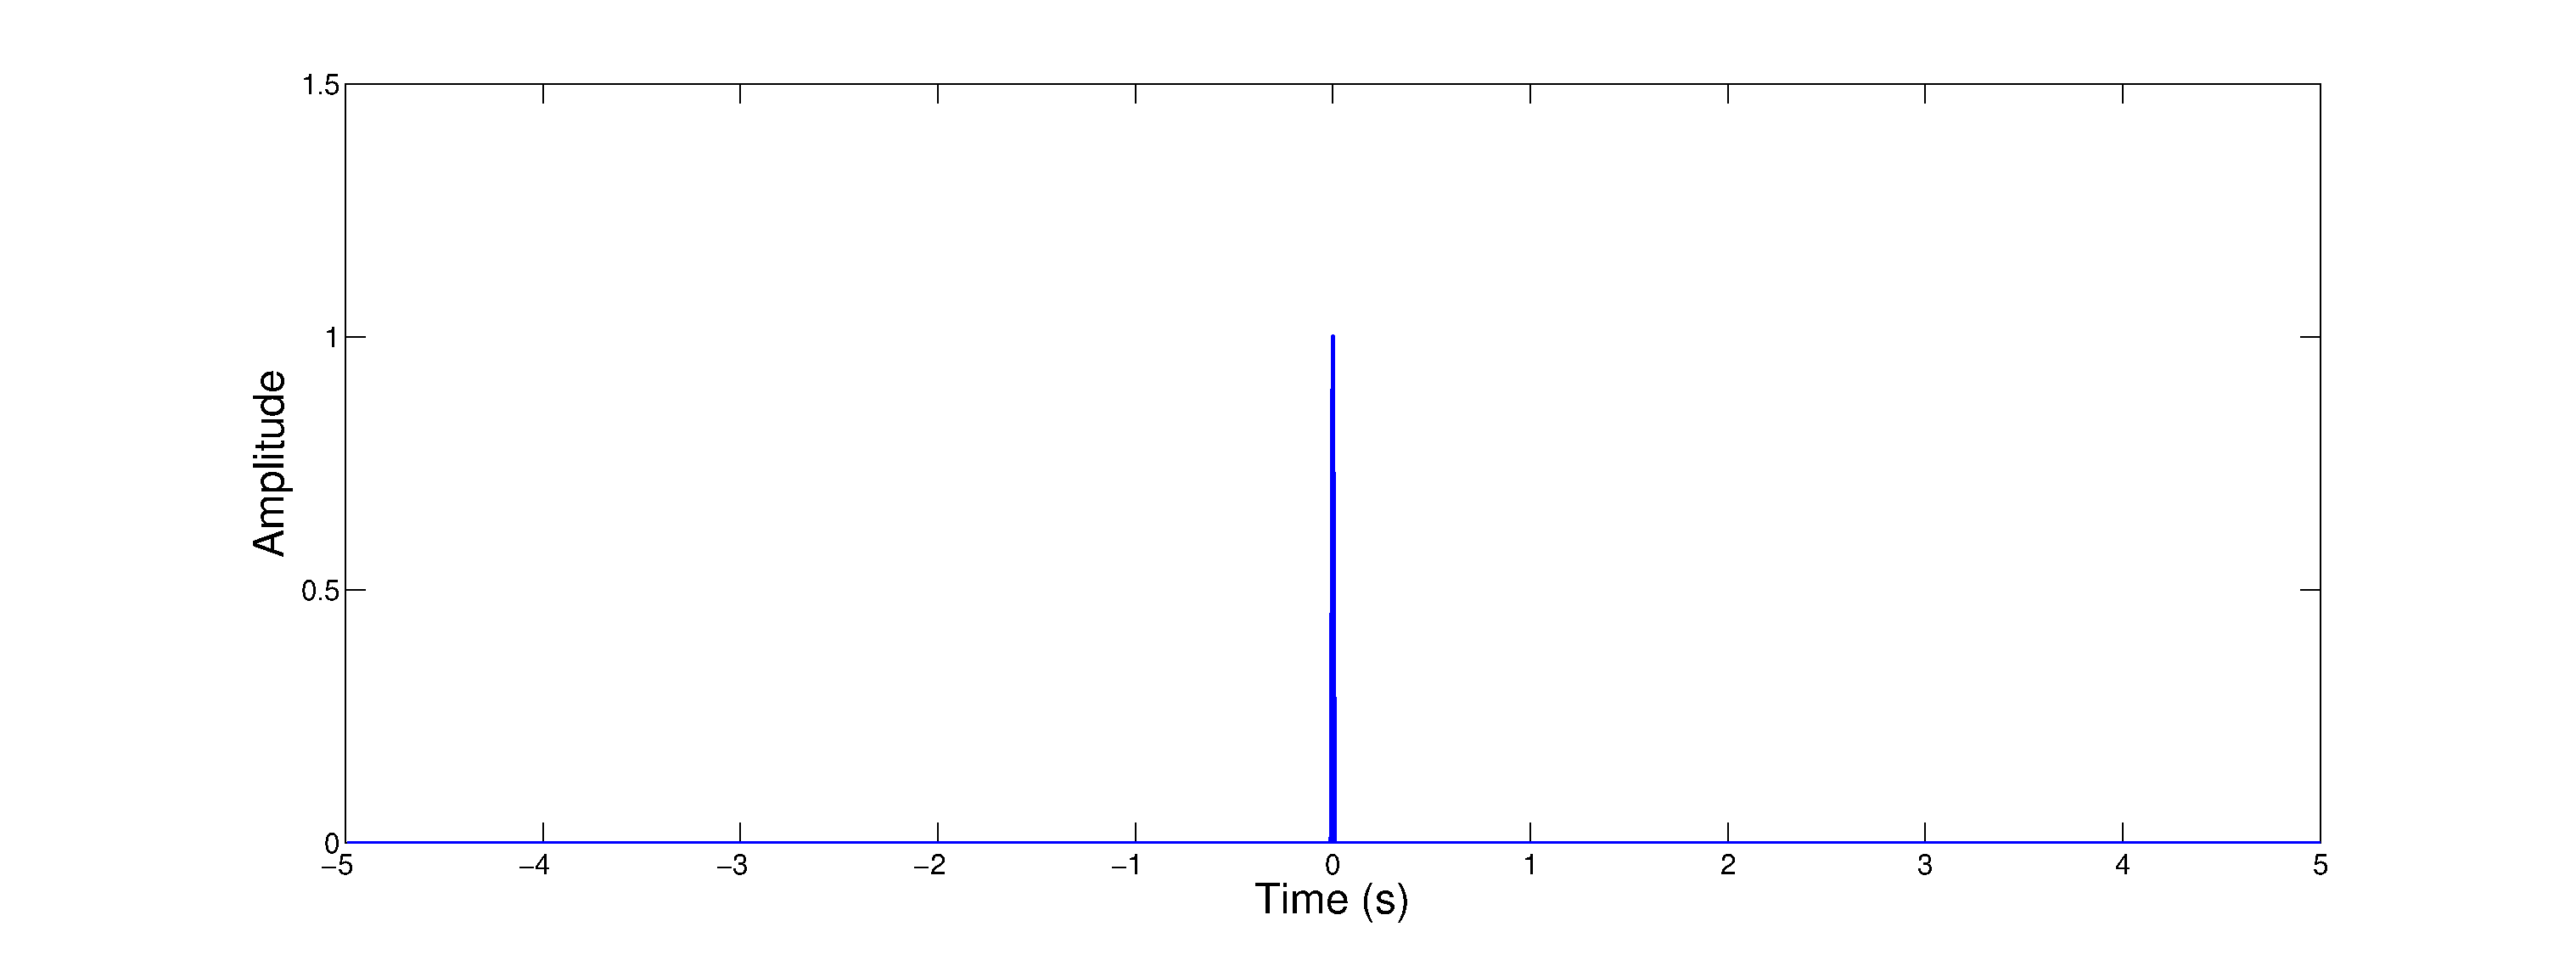
\includegraphics[width=\textwidth, keepaspectratio]{./Figures/Dirac_1D_Sig.eps} }
\subfigure[A graph showing the magnitude of the Fourier transform of the Dirac function\label{fg:Dirac:Mag}]{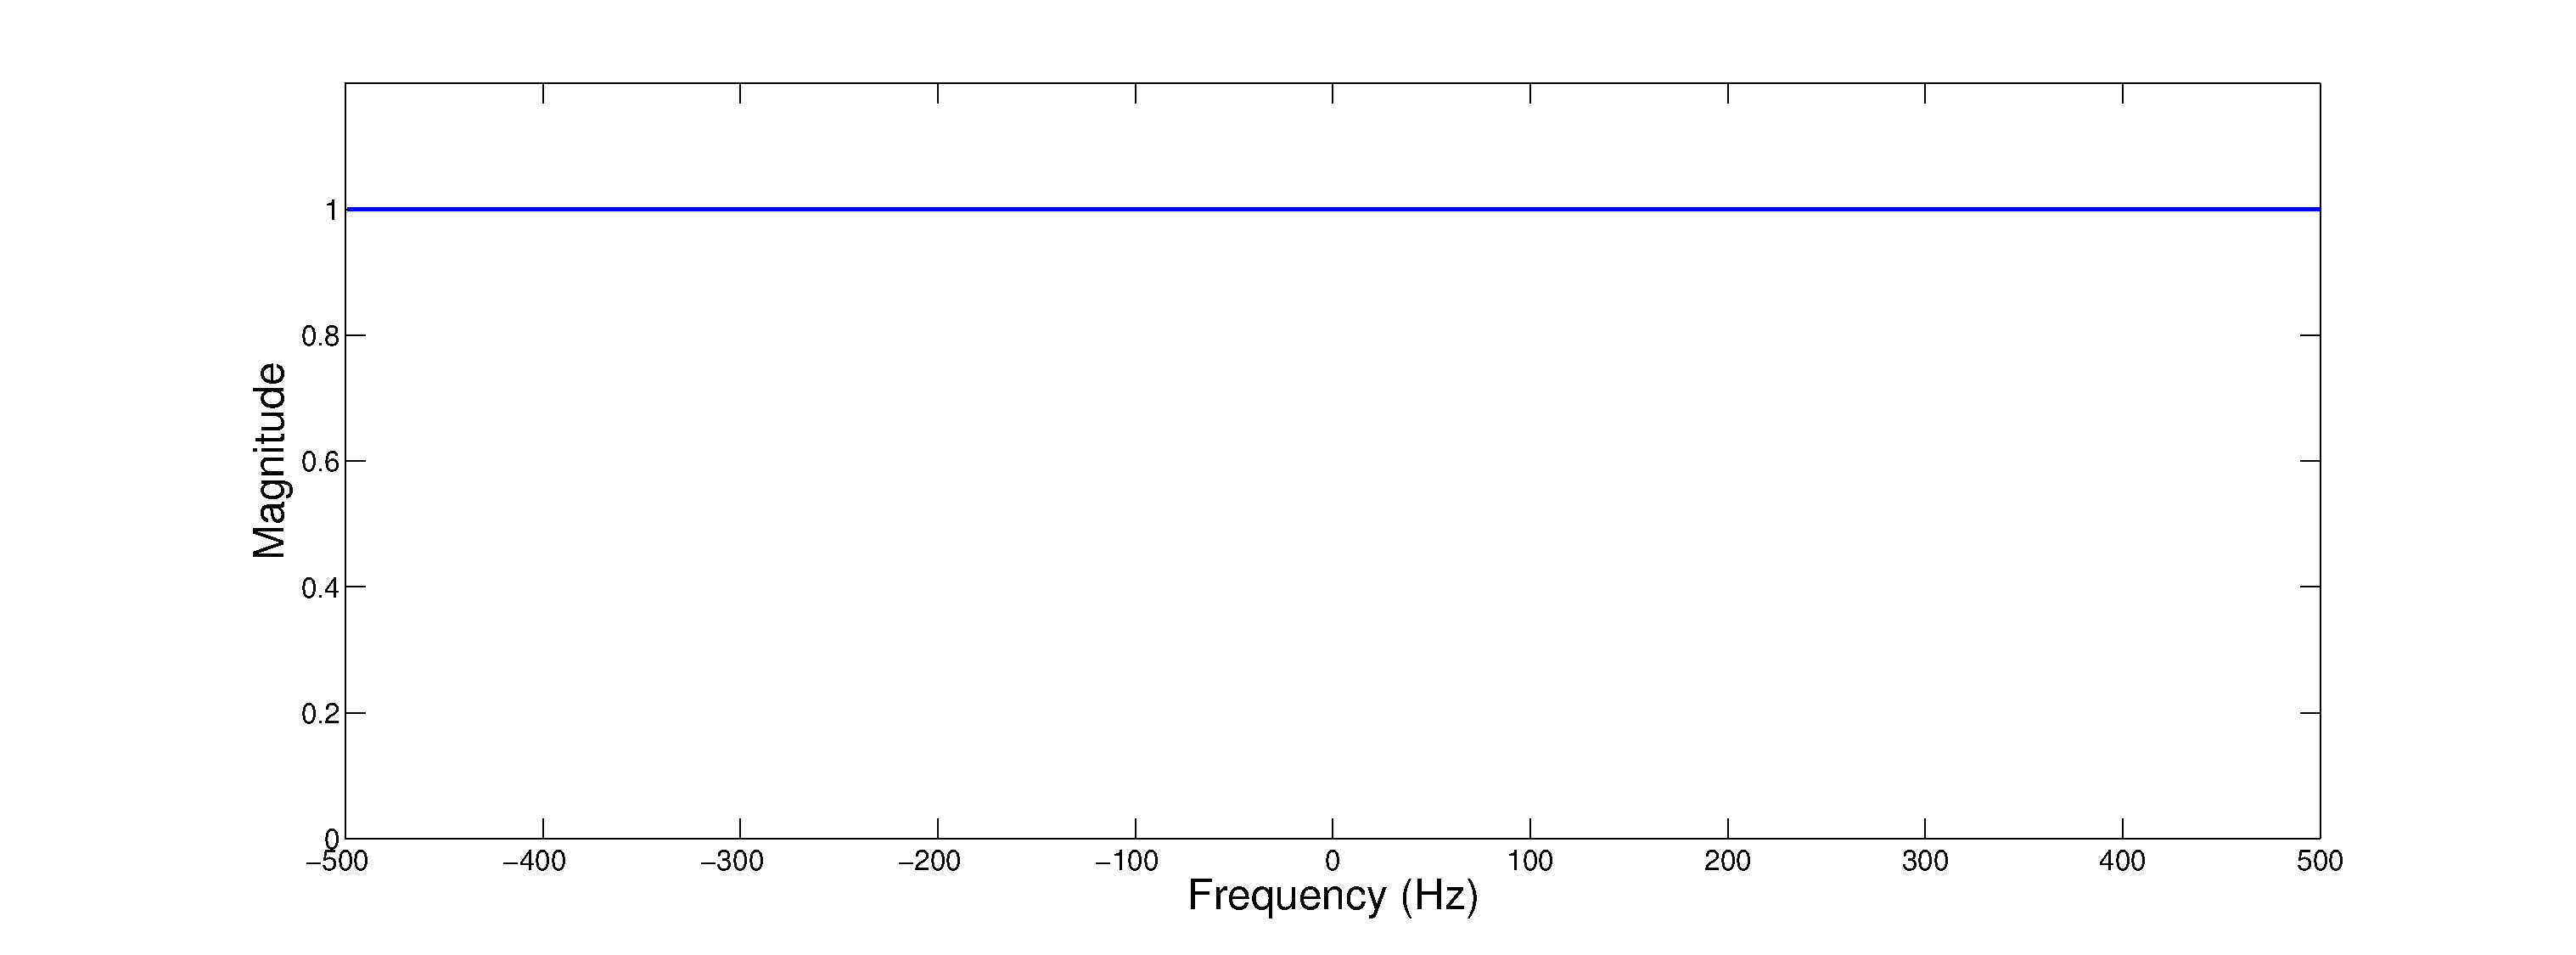
\includegraphics[width=\textwidth, keepaspectratio]{./Figures/Dirac_1D_Mag.eps} }
\subfigure[A graph showing the phase of the Fourier transform of the Dirac function\label{fg:Dirac:Phase}]{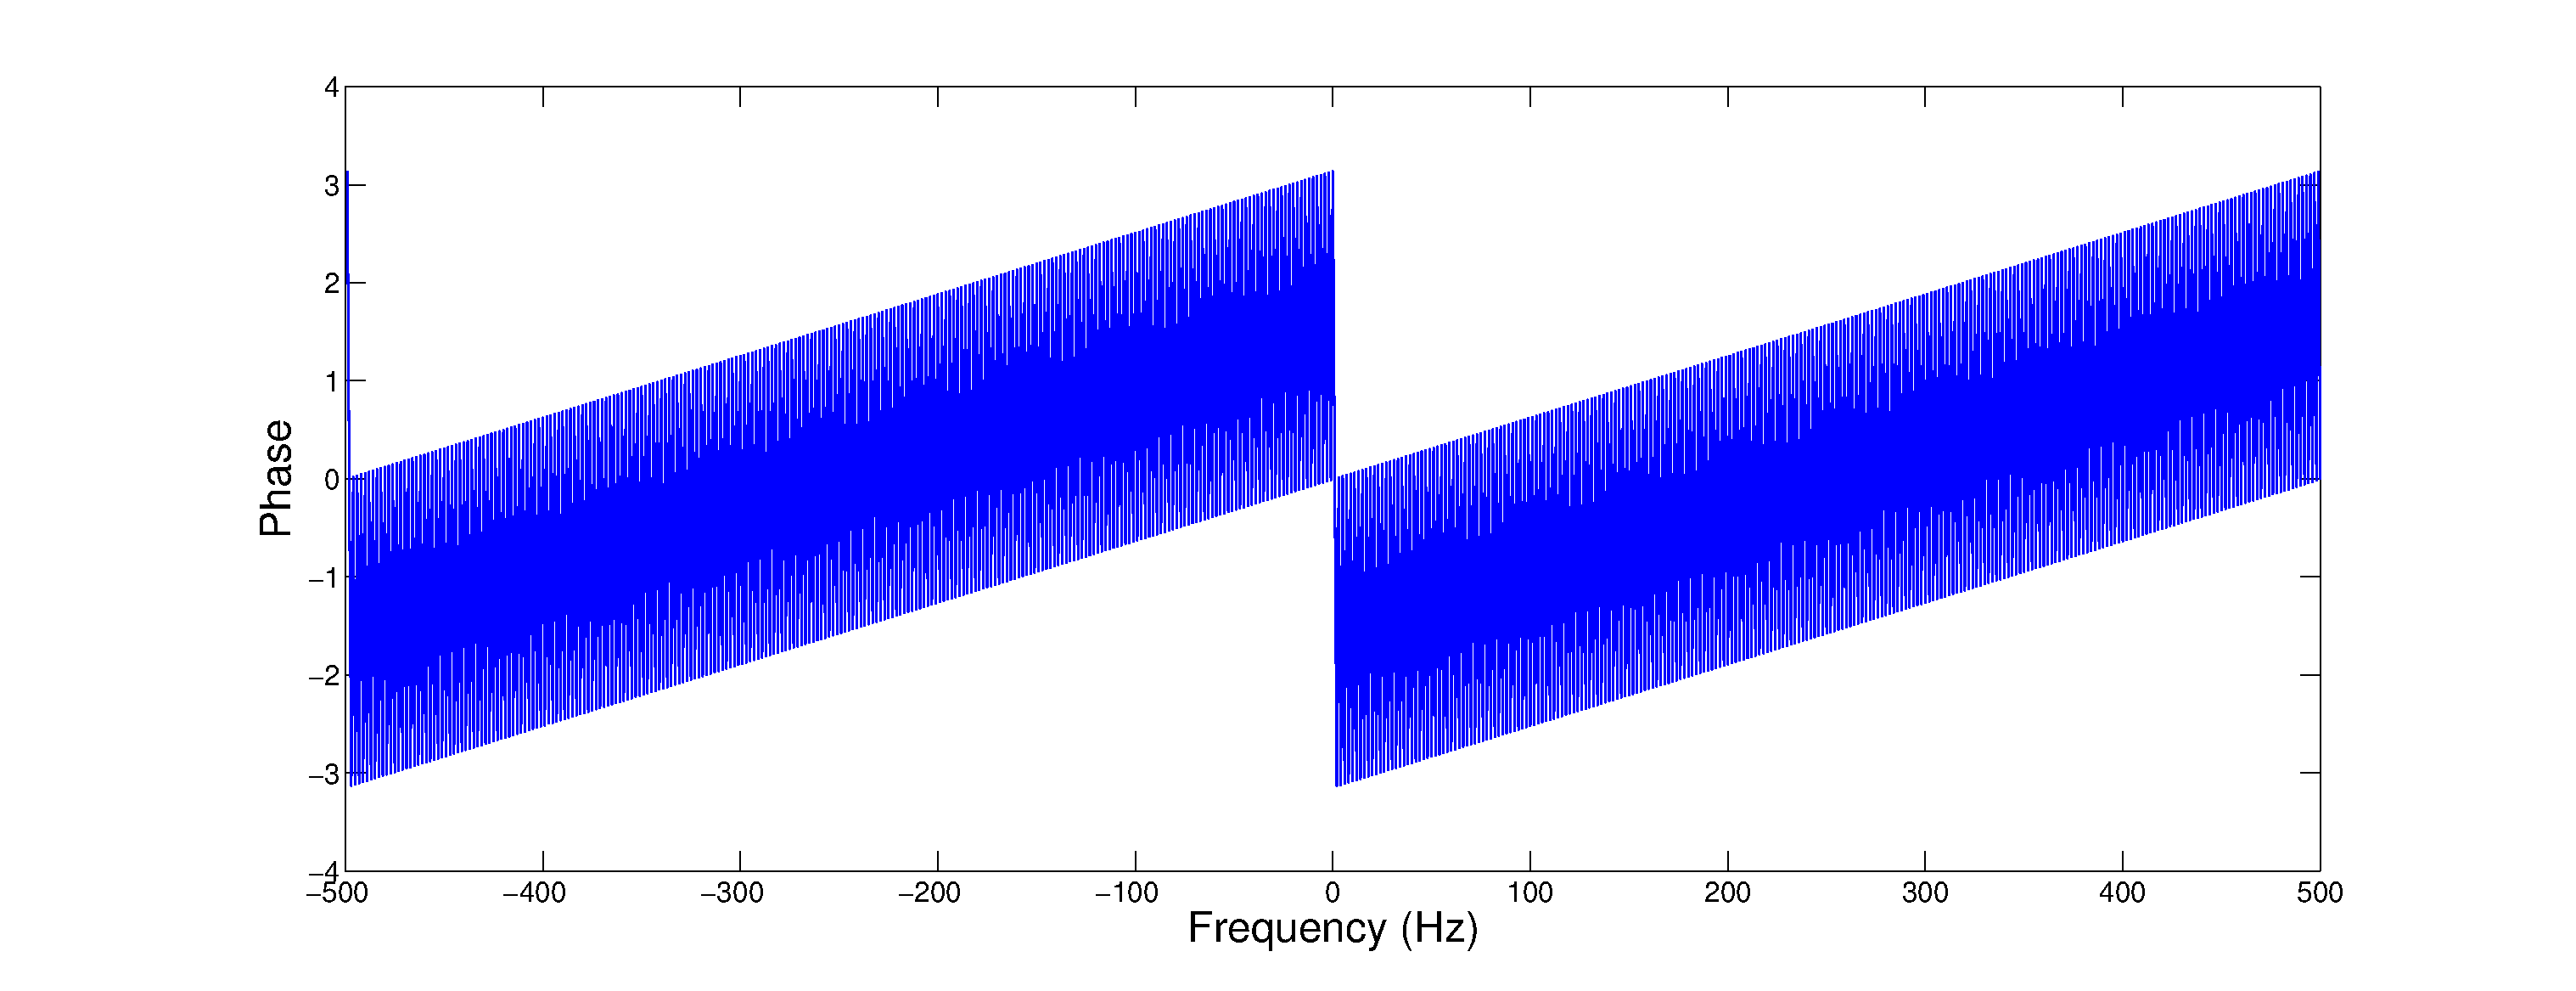
\includegraphics[width=\textwidth, keepaspectratio]{./Figures/Dirac_1D_Phase.eps} }
\caption{A Dirac function, and the phase and magnitude of its Fourier transform}
\label{fig:DiracFunctionFT}
\end{figure}

\begin{figure}
\centering
\subfigure[A graph showing rectangular pulse\label{fg:Square:Signal}]{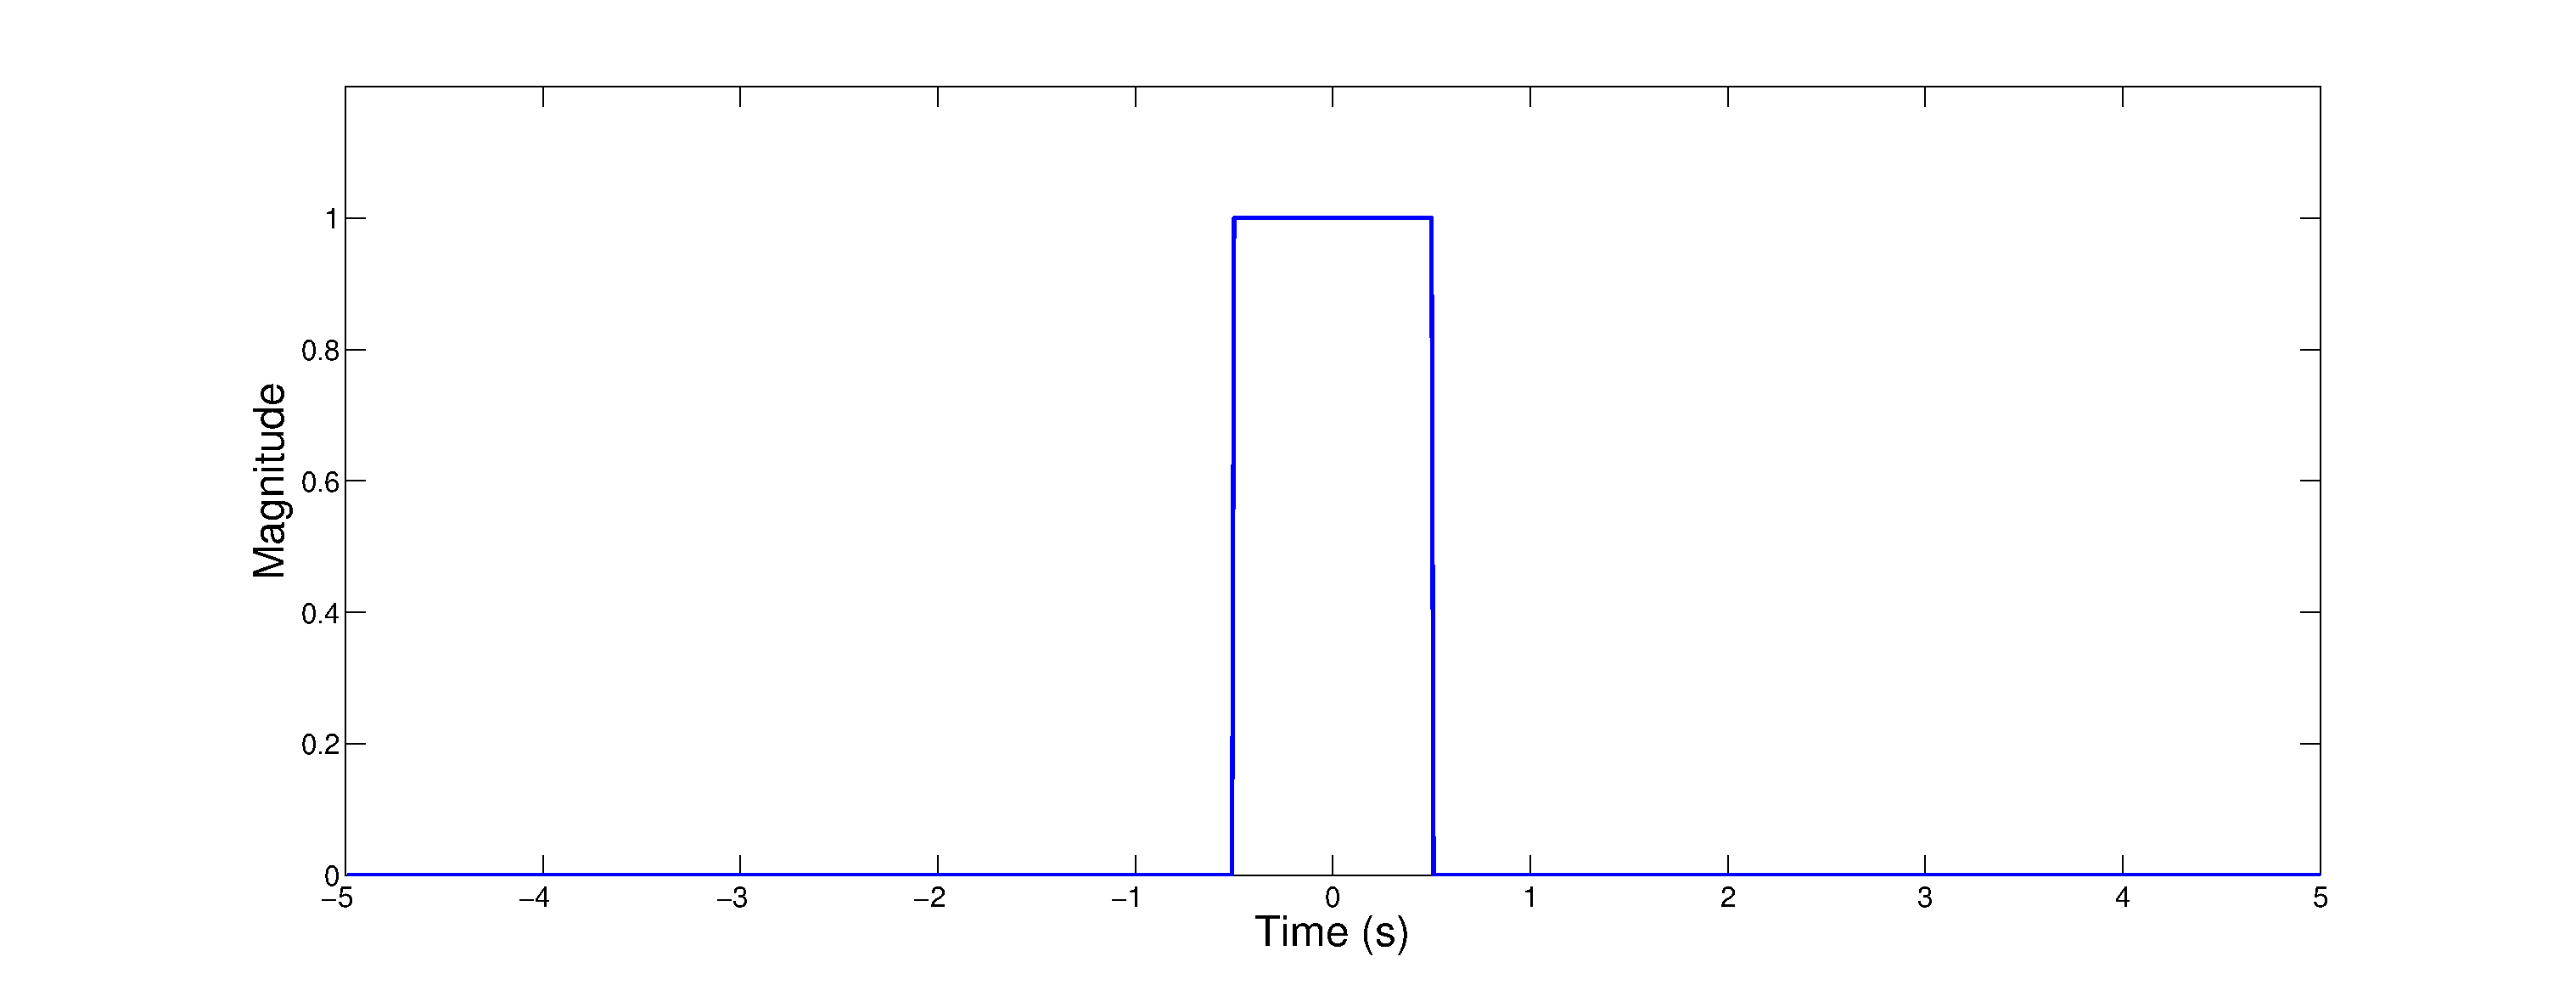
\includegraphics[width=\textwidth, keepaspectratio]{./Figures/Square_1D_Sig.eps} }
\subfigure[A graph showing the magnitude of the Fourier transform of the rectangular pulse\label{fg:Square:Mag}]{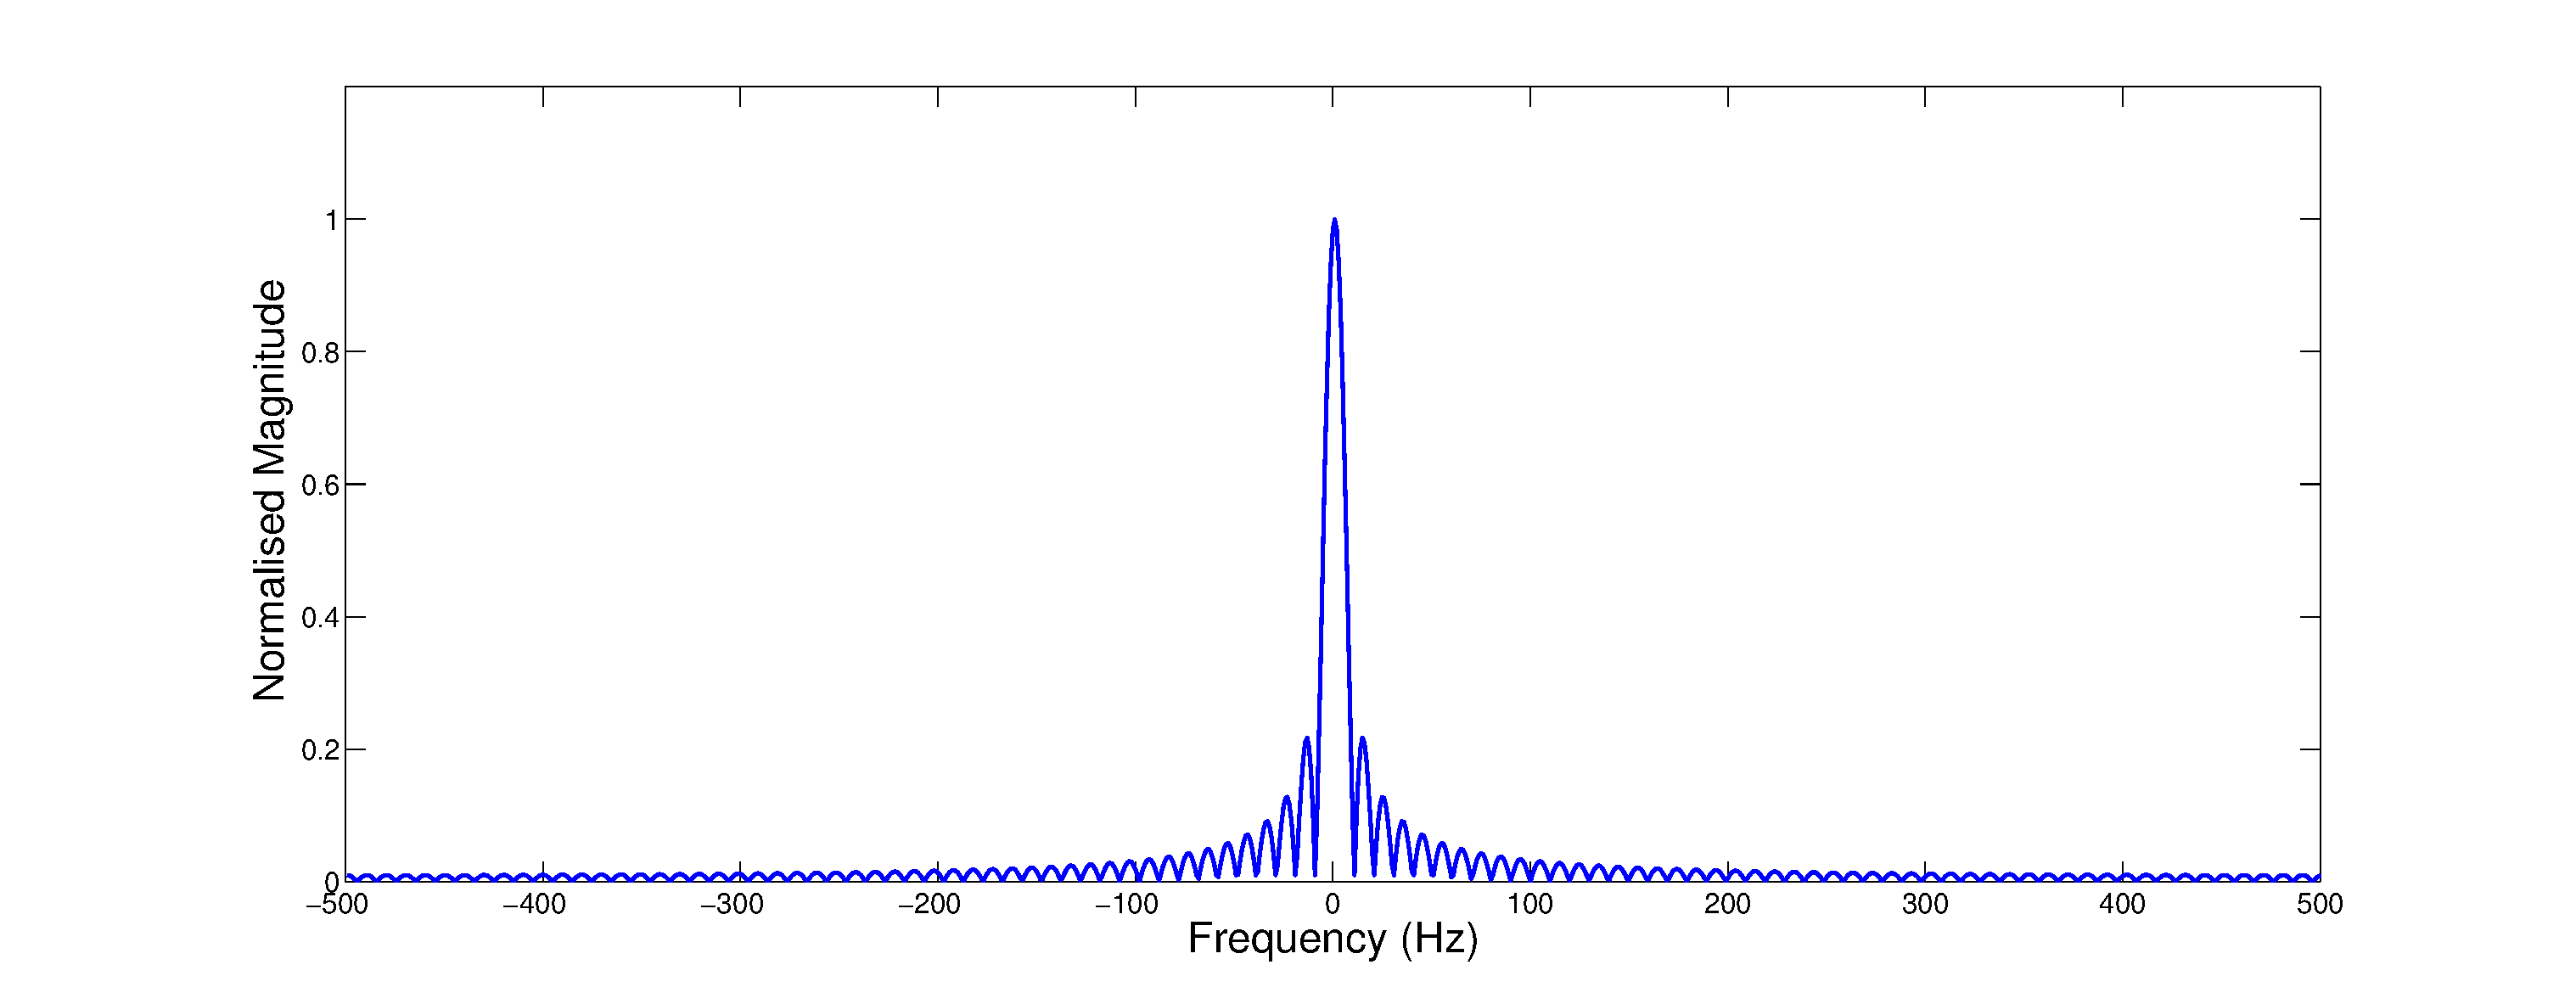
\includegraphics[width=\textwidth, keepaspectratio]{./Figures/Square_1D_Mag.eps} }
\subfigure[A graph showing the phase of the Fourier transform of the rectangular pulse\label{fg:Square:Phase}]{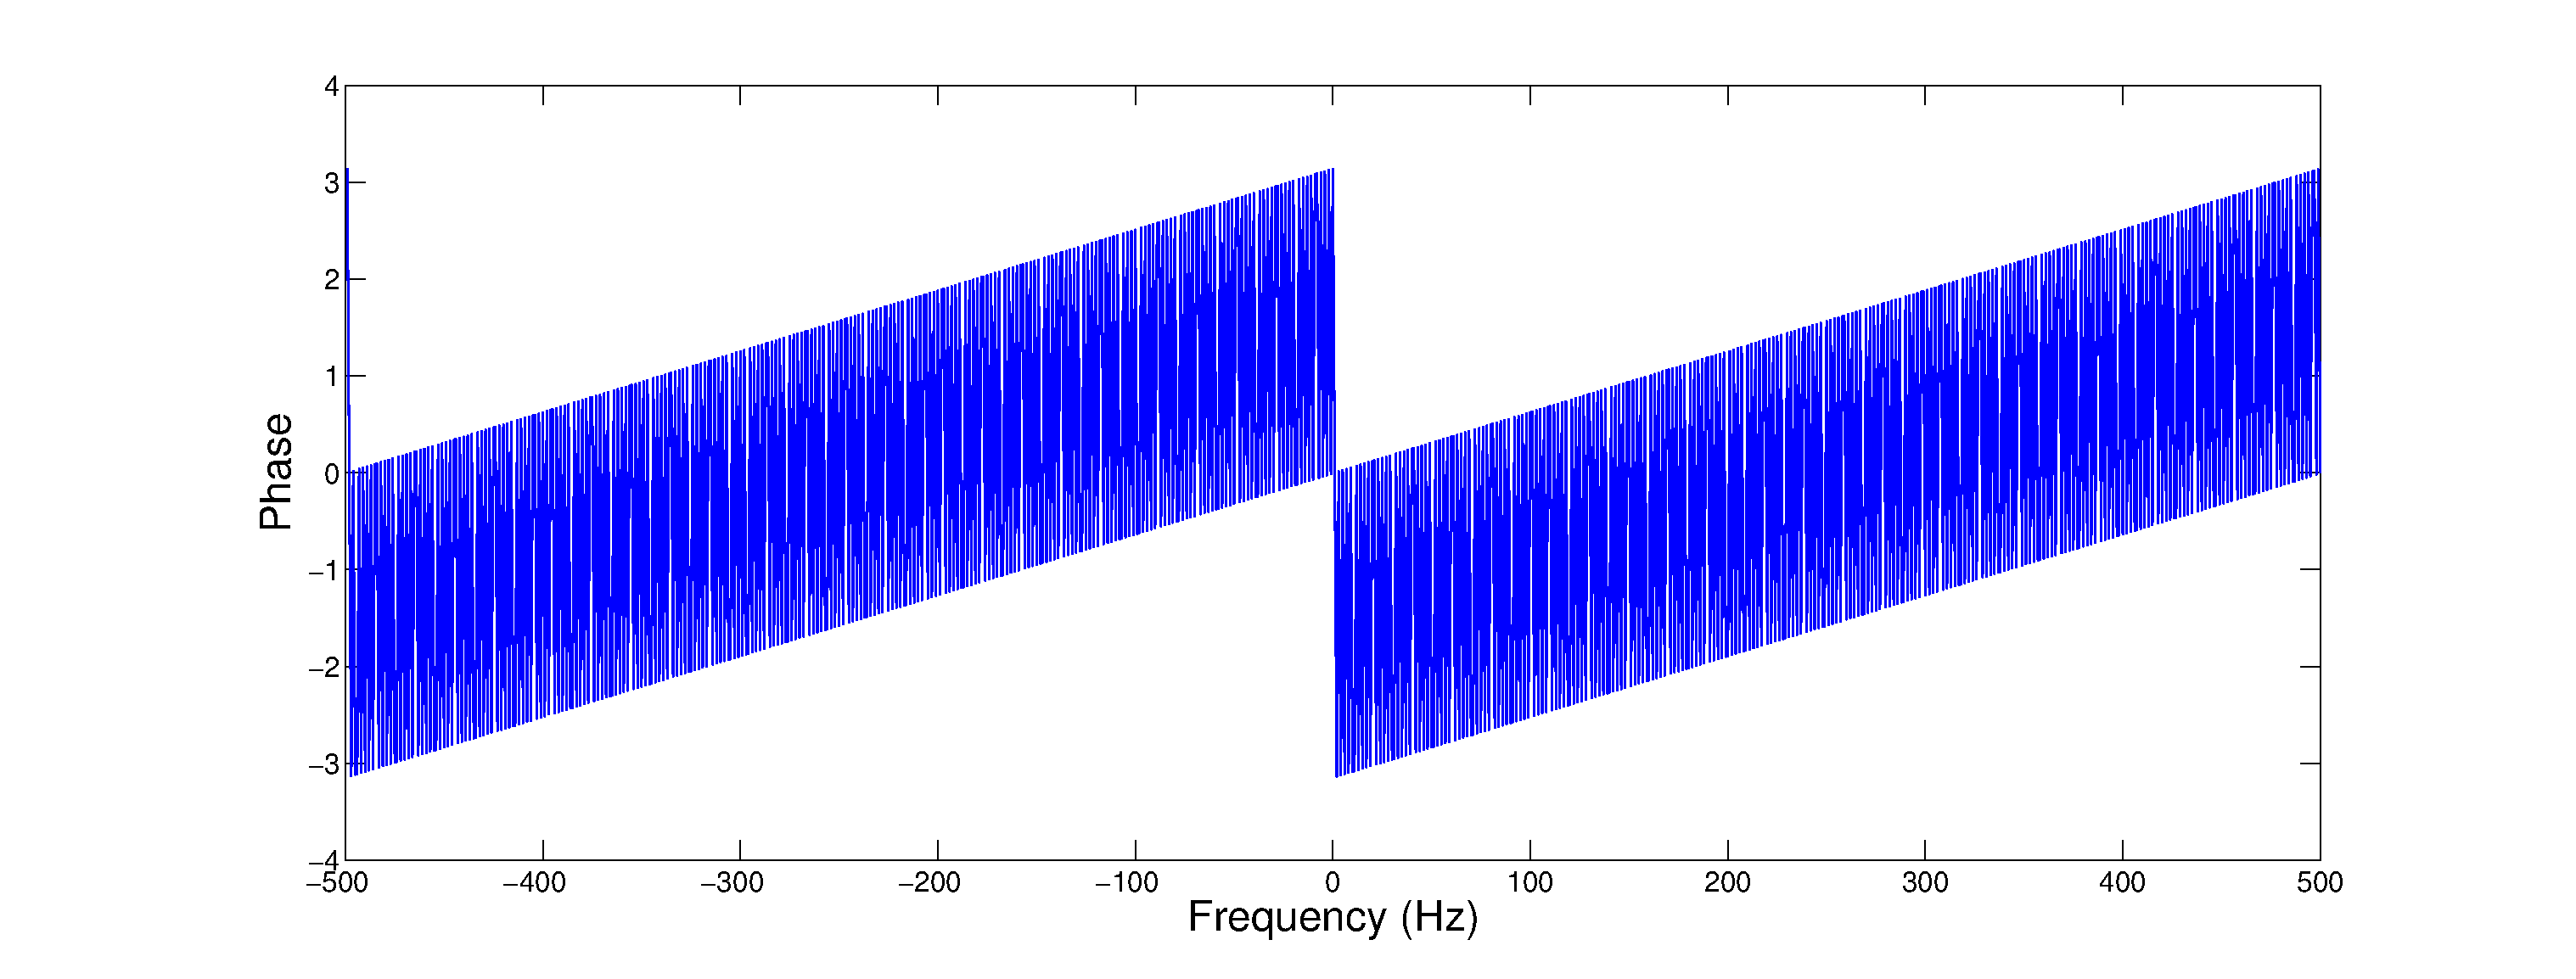
\includegraphics[width=\textwidth, keepaspectratio]{./Figures/Square_1D_Phase.eps} }
\caption{A rectangular pulse, and the phase and magnitude of its Fourier transform}
\label{fig:SquareWaveFT}
\end{figure}

The equation for the Fourier transform in Equation \eqref{eq:fourier} is for continuous time. A discrete Fourier transform (DFT) exists for finite, equally spaced samples. This is commonly used in digital systems and is defined in Equation \eqref{eq:DFT}. There exists a Fast Fourier transform (FFT) which gives exactly the same results as the DFT, but is optimised in terms of number of multiplications. The FFT is most suitable for use on microcontrollers due to the speed of calculation and the availability of code extracts. %The FFT will be used in implementation due to availability of code and speed of use. 

\begin{equation}\label{eq:DFT}
X[k] = \sum\limits_{0}^{N-1}x[n]e^{-\jmath \Omega_0 kn}
\end{equation}
\begin{center}
Where $\Omega_0$ is the sample frequency
\end{center}

A property of the Fourier transform which is of interest is the convolution theorem which states that convolution in time is multiplication in frequency and is defined mathematically in Equation \eqref{eq:ConvolutionMultiplication}. Cross correlation is defined in Equation \eqref{eq:CrossCorrelation} and related to convolution by Equation \eqref{eq:CrossCorrelation}. With images, $f(t)$ is a real signal, its conjugate is exactly the same, $f(t) \equiv f^*(t)$, given that $f(t) \in \Re$. Fourier transforms can be used to calculate cross correlation more efficiently, by multiplying the Fourier transform of an image by the reversed template.% This means that to compute a cross correlation, the Fourier transform of the image and the reversed template can be used and multiplied together. 


\begin{equation}\label{eq:ConvolutionMultiplication}
\int\limits_{-\infty}^{\infty}f(\tau)g(t-\tau)d\tau = f(t) \ast g(t) = X(f)\cdot Y(f)
\end{equation}
\begin{equation}\label{eq:CrossCorrelation}
\int\limits_{-\infty}^{\infty}f^*(\tau)g(t+\tau)d\tau = f(t) \star g(t) = f'(-t) \ast g(t) = X(-f)\cdot Y(f)
\end{equation}

%\begin{equation}\label{eq:CCtoConv}
%f(t) \star g(t) = f(t) \ast g(-t) = F(f) \cdot G(-f)
%\end{equation}

%\inote{example of convolution used as correlation. Include some pretty graphs}
\subsection{Two Dimensional Fast Fourier Transform}
A two dimensional (2D) Fourier transform exists for analysing 2D signals, such as an image. The Fourier Transform is shown in Equation \eqref{eq:2dFT} and the discrete version is shown in Equation \eqref{eq:2dDFT}

\begin{equation}\label{eq:2dFT}
F(u,v) = \frac{1}{2\pi}\int\limits_{-\infty}^{\infty}\int\limits_{-\infty}^{\infty}f(x,y)e^{-2\pi\jmath (xu+yv)}dxdy
\end{equation}
\begin{equation}\label{eq:2dDFT}
F(u,v) = \frac{1}{N} \sum\limits_{x=0}^{N-1}\sum\limits_{y=0}^{N-1}f(x,y)e^{-\frac{2\pi\jmath (xu+yv)}{N}} \; \; \; \; \; x,y,u,v \in \left\lbrace 0\dots N-1\right\rbrace
\end{equation}

Figures \ref{fig:2DDiracFunctionFT} and \ref{fig:2DSquareWaveFT} show the 2D equivalent test signals of Figures \ref{fg:Dirac:Signal} and \ref{fg:Square:Signal}, and the phase and magnitudes of their Fourier Transforms. There is a direct similarity between the 1D and 2D spectra; the magnitudes of the Dirac (Figures \ref{fg:Dirac:Mag} and \ref{fg:Dirac2D:Mag}) are both constant values and the rectangular pulses both have a modulus sinc function magnitude (Figures \ref{fg:Square:Signal} and \ref{fg:Square2D:Signal}). 

\begin{figure}
\centering
\subfigure[An image of a 2D Dirac function\label{fg:Dirac2D:Signal}]{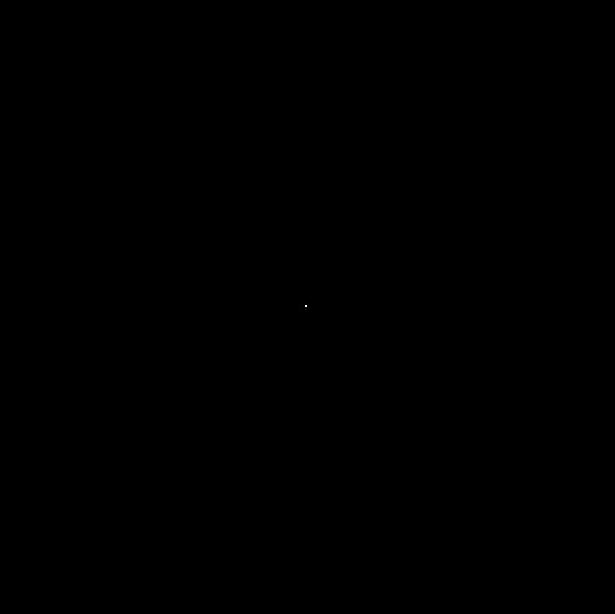
\includegraphics[width=10cm, keepaspectratio]{./Figures/Dirac_2D_Sig.jpg} }
\subfigure[An image of the magnitude of the Fourier transform of the 2D Dirac function\label{fg:Dirac2D:Mag}]{\fbox{
\includegraphics[width=(\textwidth / 2)-1cm, keepaspectratio]{./Figures/Dirac_2D_Mag.jpg} }}
\subfigure[An image of the phase of the Fourier transform of the 2D Dirac function\label{fg:Dirac2D:Phase}]{
\includegraphics[width =(\textwidth / 2)-1cm, keepaspectratio]{./Figures/Dirac_2D_Phase.jpg} }
\caption{A 2D Dirac signal, and the phase and magnitude of its Fourier transform}
\label{fig:2DDiracFunctionFT}
\end{figure}

\begin{figure}
\centering
\subfigure[An image of the 2D rectangular pulse\label{fg:Square2D:Signal}]{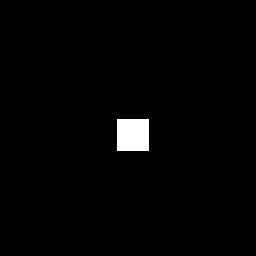
\includegraphics[width =10cm, keepaspectratio]{./Figures/Square_2D_Sig.jpg} }
\subfigure[An image of the magnitude of the Fourier transform of the 2D rectangular pulse\label{fg:Square2D:Mag}]{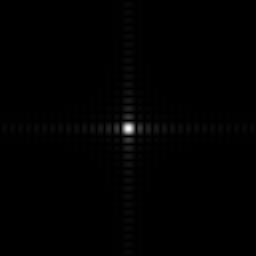
\includegraphics[width =(\textwidth / 2)-1cm, keepaspectratio]{./Figures/Square_2D_Abs.jpg} }
\subfigure[An image of the phase of the Fourier transform of the 2D rectangular pulse\label{fg:Square2D:Phase}]{
\includegraphics[width =(\textwidth / 2)-1cm, keepaspectratio]{./Figures/Square_2D_Phase.jpg} }
\caption{A 2D rectangular pulse signal, and the phase and magnitude of its Fourier transform}
\label{fig:2DSquareWaveFT}
\end{figure}

The 2D Fourier transform can also be optimised to a FFT algorithm in a similar way to the 1D case. However, this algorithm, sometimes referred to as the Butterfly transform, can only be applied to images with equal dimensions that are a power of 2, without extra effort \citep{nixon2012feature}. The algorithm utilises the separability property of the Fourier transform. 

The 2D FFT can be implemented using a 1D FFT as follows:
\begin{enumerate}
\item Calculate the 1D FFT of each of the rows of the 2D data. (An FFT of data of length $n$ returns an array, also of length $n$)
\item Calculate the 1D FFT of each of the columns of the 2D data returned from the previous step.
\end{enumerate}
Total number of FFTs done is $2n$ where $n$ is the height/width of the image. 
\inote{Maybe make a figure to help explain?}
\subsection{Implementing the FFT}
%\inote{Include and explain code}
The Atmel Software Framework \citep{Atmel:ASF} included a digital signal processing library. This contained functions to compute the FFT of a real or complex array, the inverse FFT and the magnitude of complex data. Further restrictions are imposed by the DSP library used as the data must be in fixed point notation and with a length of an even power of 2. This gives a usable dimension of $256px \times 256px$ for processing images on the AVR. Though the height of an image from the OV7670 camera is $240$ pixels, the image can be transformed so that it repeats for 16 rows at the bottom as the Fourier transform works on an assumption of the data being periodic.

A function was made, called \textit{FFT2DCOMPLEX}, to realise the 2D FFT on the microcontroller. The FFT function requires the data to be 4 byte aligned (A\_ALIGNED) and of type \textit{dsp16\_complex\_t}. The data must be given in fixed point notation and it are returned in fixed point notation. A 16 bit representation was chosen over 32 bit due to more functions being available. 


\subsection{Testing of the FFT on AVR}
\subsubsection{1D FFT Test}
A Dirac function and a rectangular pulse were used as test signals. 

Figure \ref{fig:AVR:FFT:Dirac:Input} shows the input signal given to the AVR. It is a 256 long array of a Dirac function. This was then converted to the internally defined fixed point notation and passed through the Fourier transform method. The resulting complex array was then saved to a CSV file and read into MATLAB. Figure \ref{fig:AVR:FFT:Dirac:Output} shows the calculated phase and magnitude plots of the output complex array. The magnitude is relatively flat and around the value of 1. In comparison with Figure \ref{fg:Dirac:Mag}, they are relatively similar. The phase, however, seems to be very different. Figure \ref{fg:Dirac:Phase} shows what was expected, but the two phase results appear to be quite different. This could be due to MATLAB having more accurate algorithms and a more accurate representation than the 16 bit fixed point used on the AVR. However, using a function in the DSP library to calculate the magnitude, the spectrum in Figure \ref{fig:AVR:FFT:Dirac:Mag} is obtained. This, though is not a magnitude of exactly $1.0$ as expected, is completely flat and it is computed from the same transformed data. This suggests that there is some internal compensation in the algorithms. The actual value in Figure \ref{fig:AVR:FFT:Dirac:Mag} is $0.9897$ to 4 decimal places giving an overall error of $1.03\%$. 

Figures \ref{fig:AVR:FFT:Square:Input}, \ref{fig:AVR:FFT:Square:Output} and \ref{fig:AVR:FFT:Square:Mag} show the similar outputs from the AVR when transforming the rectangular pulse. The result was renormalised from fixed point notation and the data was shifted so that the centre of the plot is frequency 0.  Again, it can be seen that the magnitude calculated from the complex output (Figure \ref{fig:AVR:FFT:Square:Output}) is different to the result when the magnitude is calculated on the AVR (Figure \ref{fig:AVR:FFT:Square:Mag}). There are also differences in the result from the AVR and the result from MATLAB in Figure \ref{fig:SquareWaveFT}, which can, again, be attributed to the algorithms. 

\begin{figure}
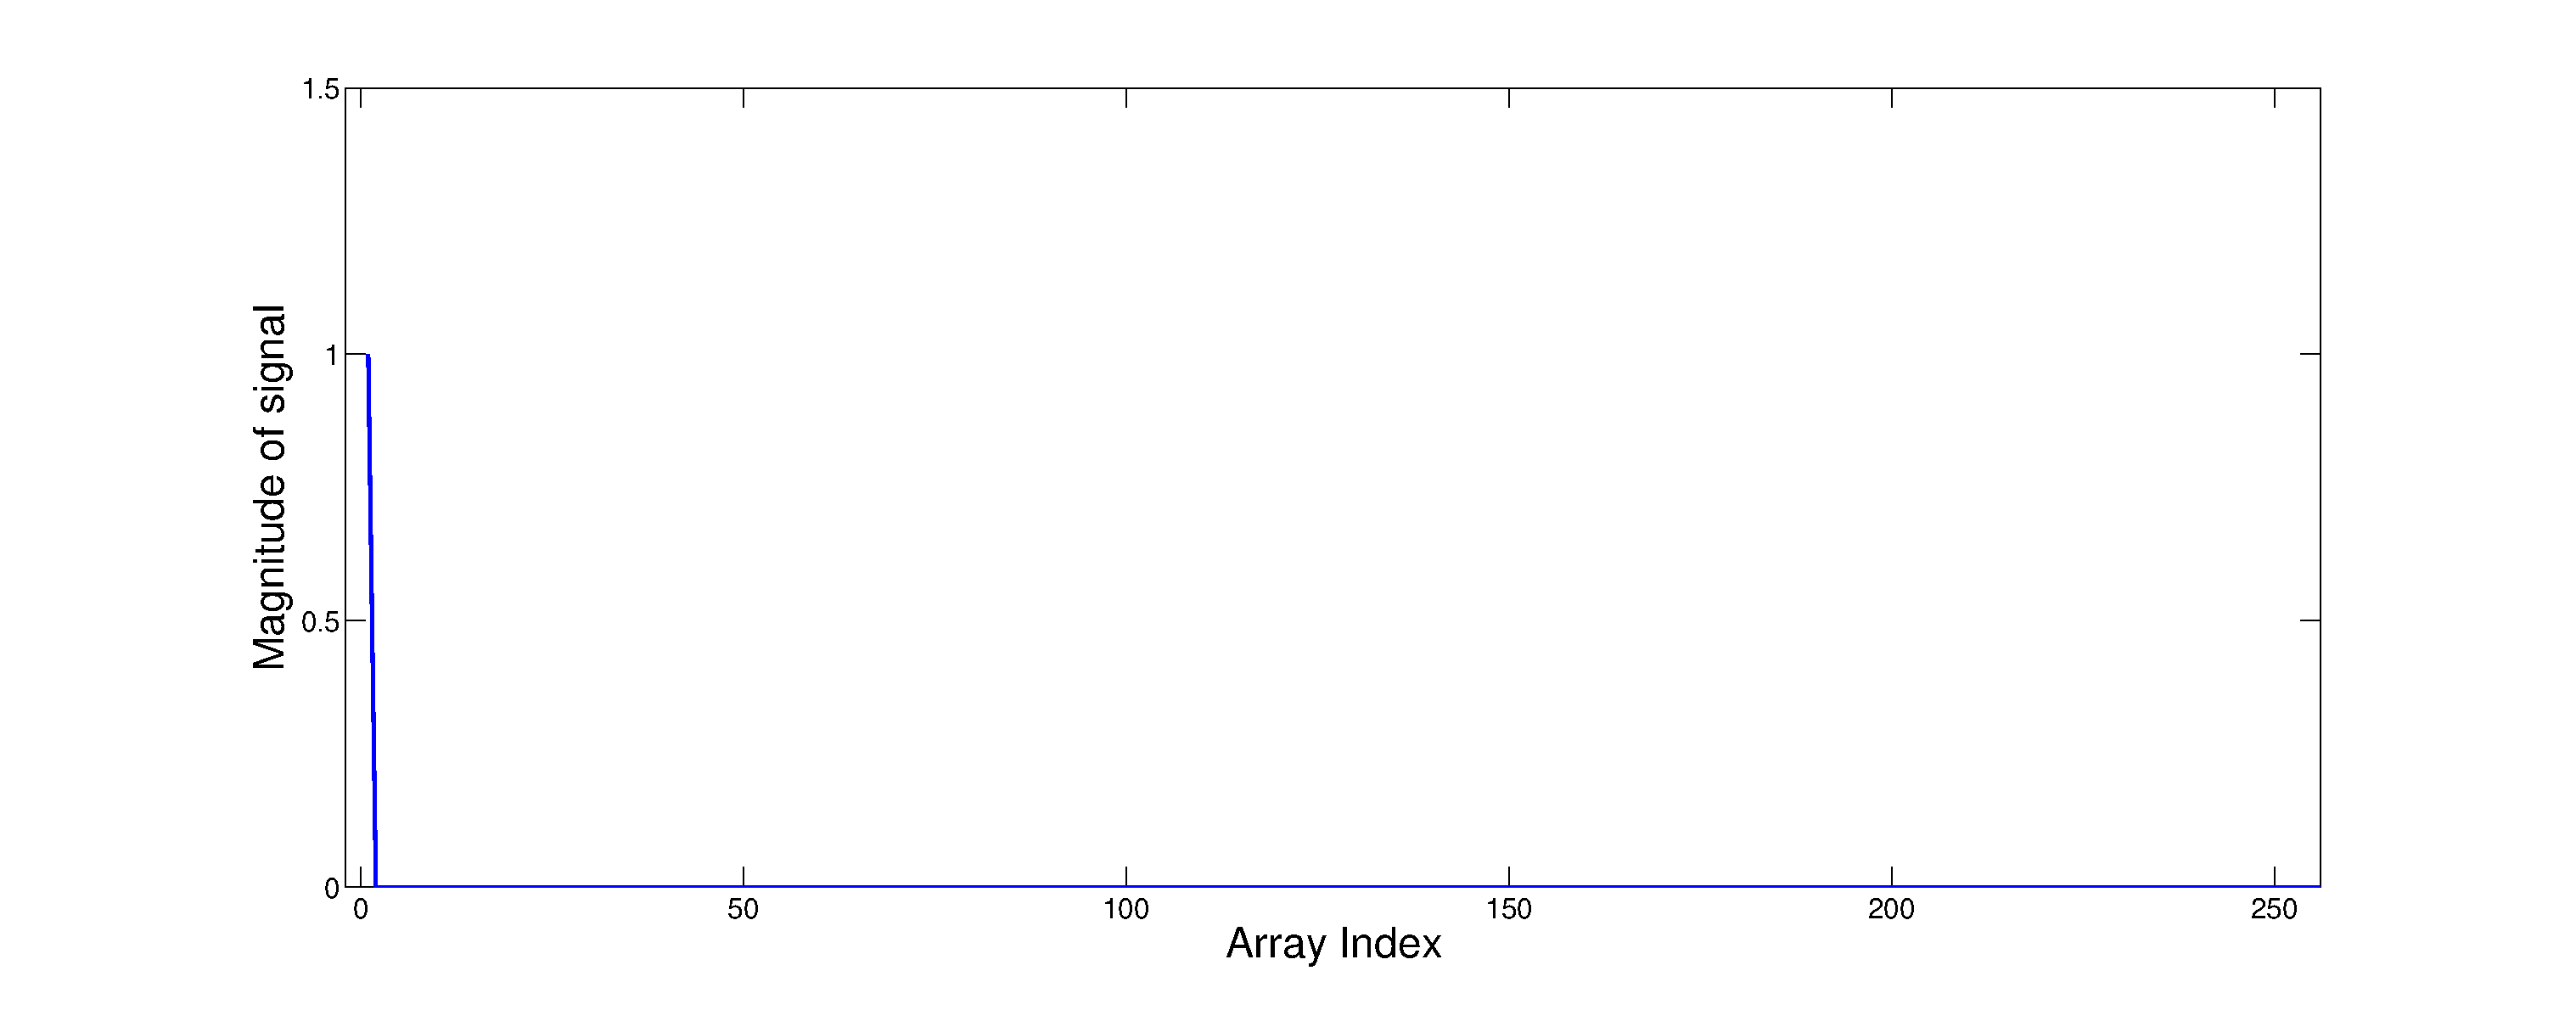
\includegraphics[width=\textwidth]{./Figures/AVR_FFT_Dirac_Input.eps}
\caption{Input Dirac signal for AVR fast Fourier transform}
\label{fig:AVR:FFT:Dirac:Input}
\end{figure}
\begin{figure}
\subfigure[Magnitude of the complex output from the AVR]{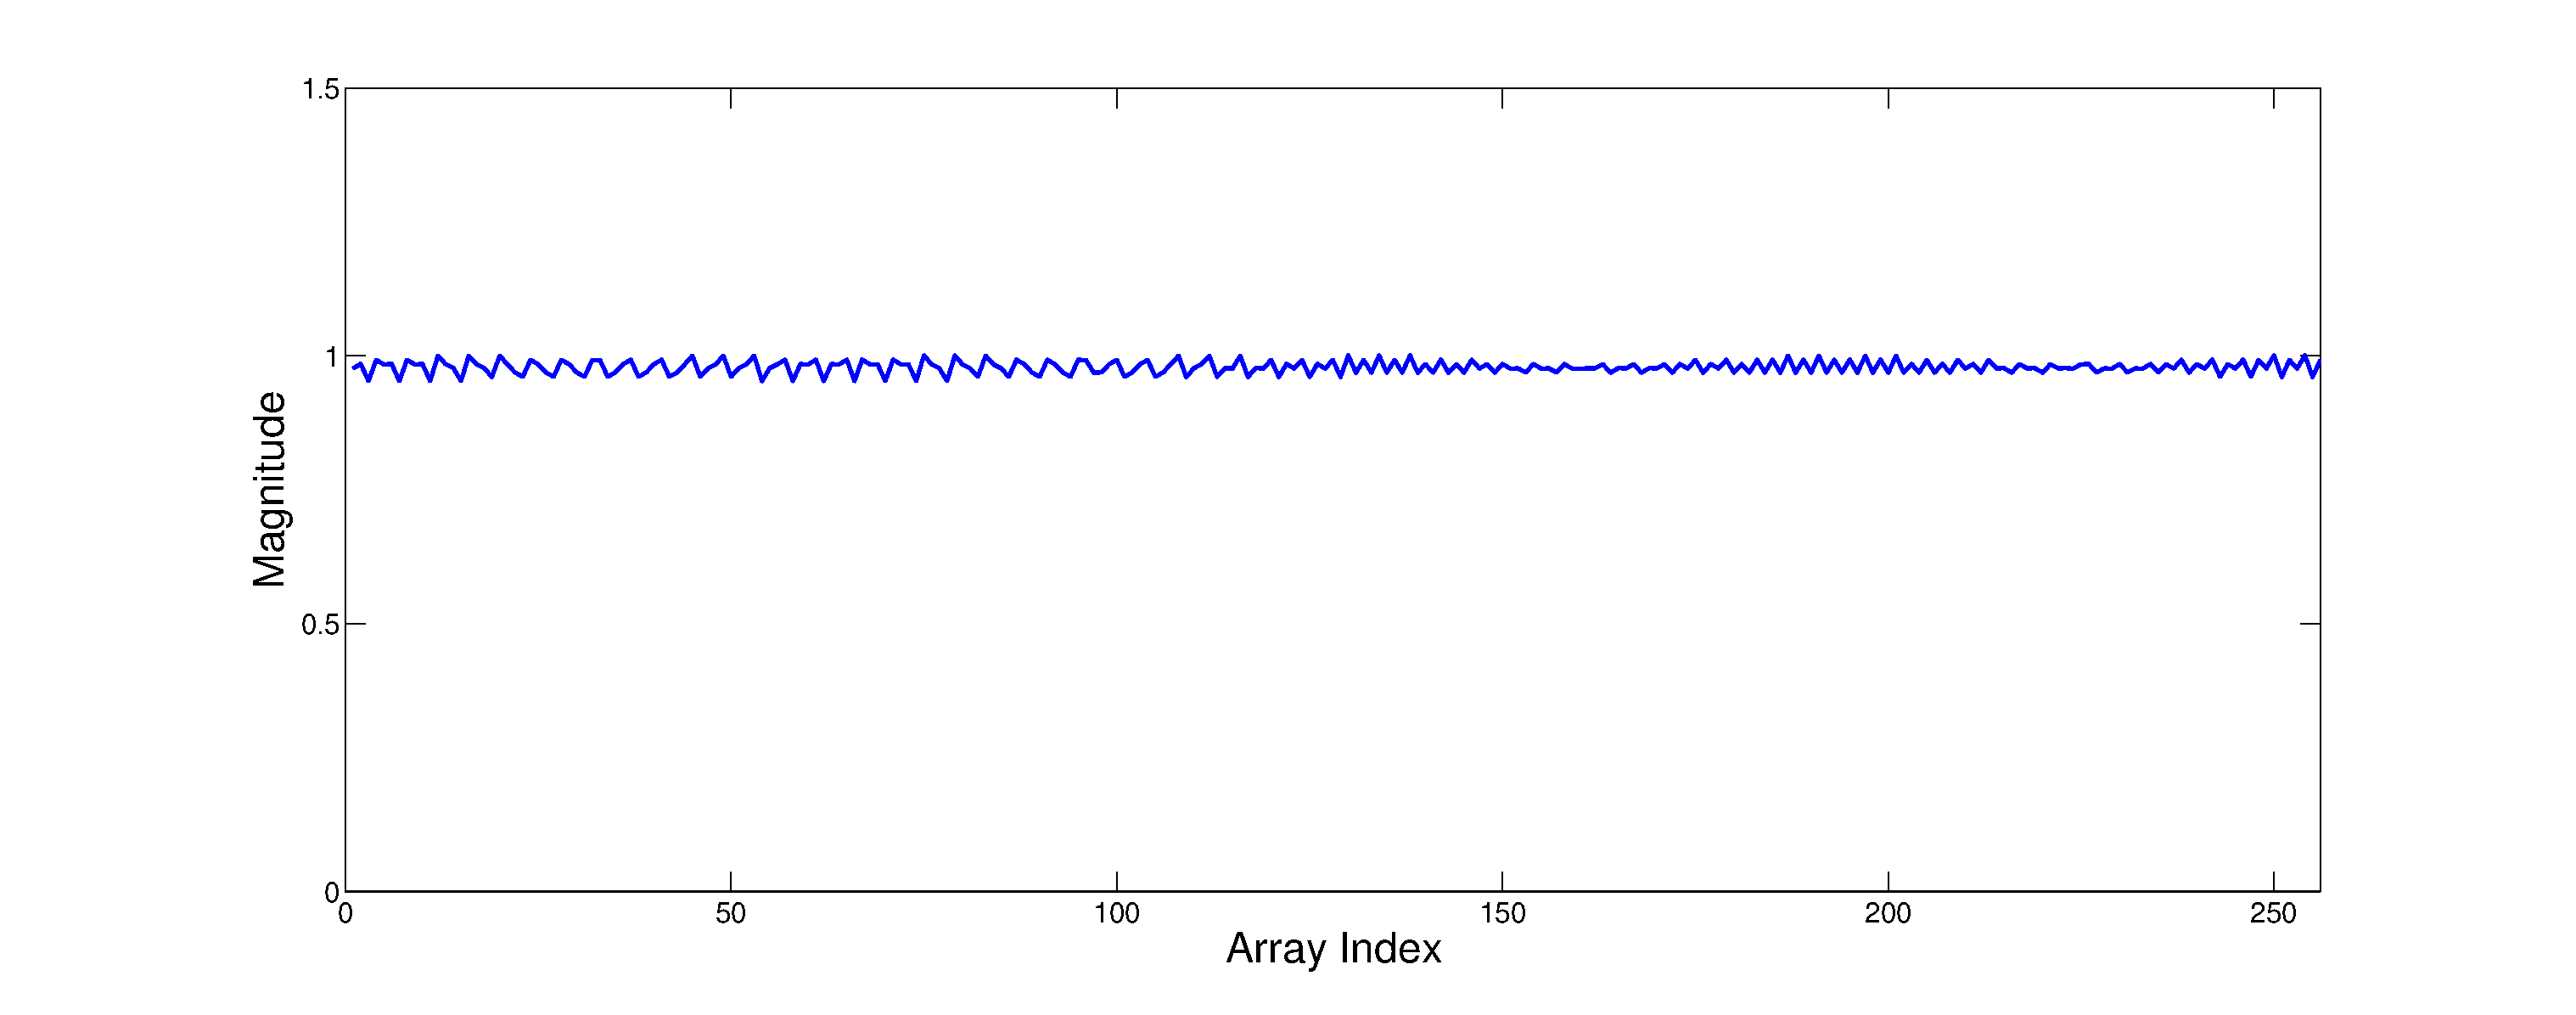
\includegraphics[width =\textwidth, keepaspectratio]{./Figures/AVR_FFT_Dirac_Complex_Mag.eps} }
\subfigure[Phase of the complex output from the AVR]{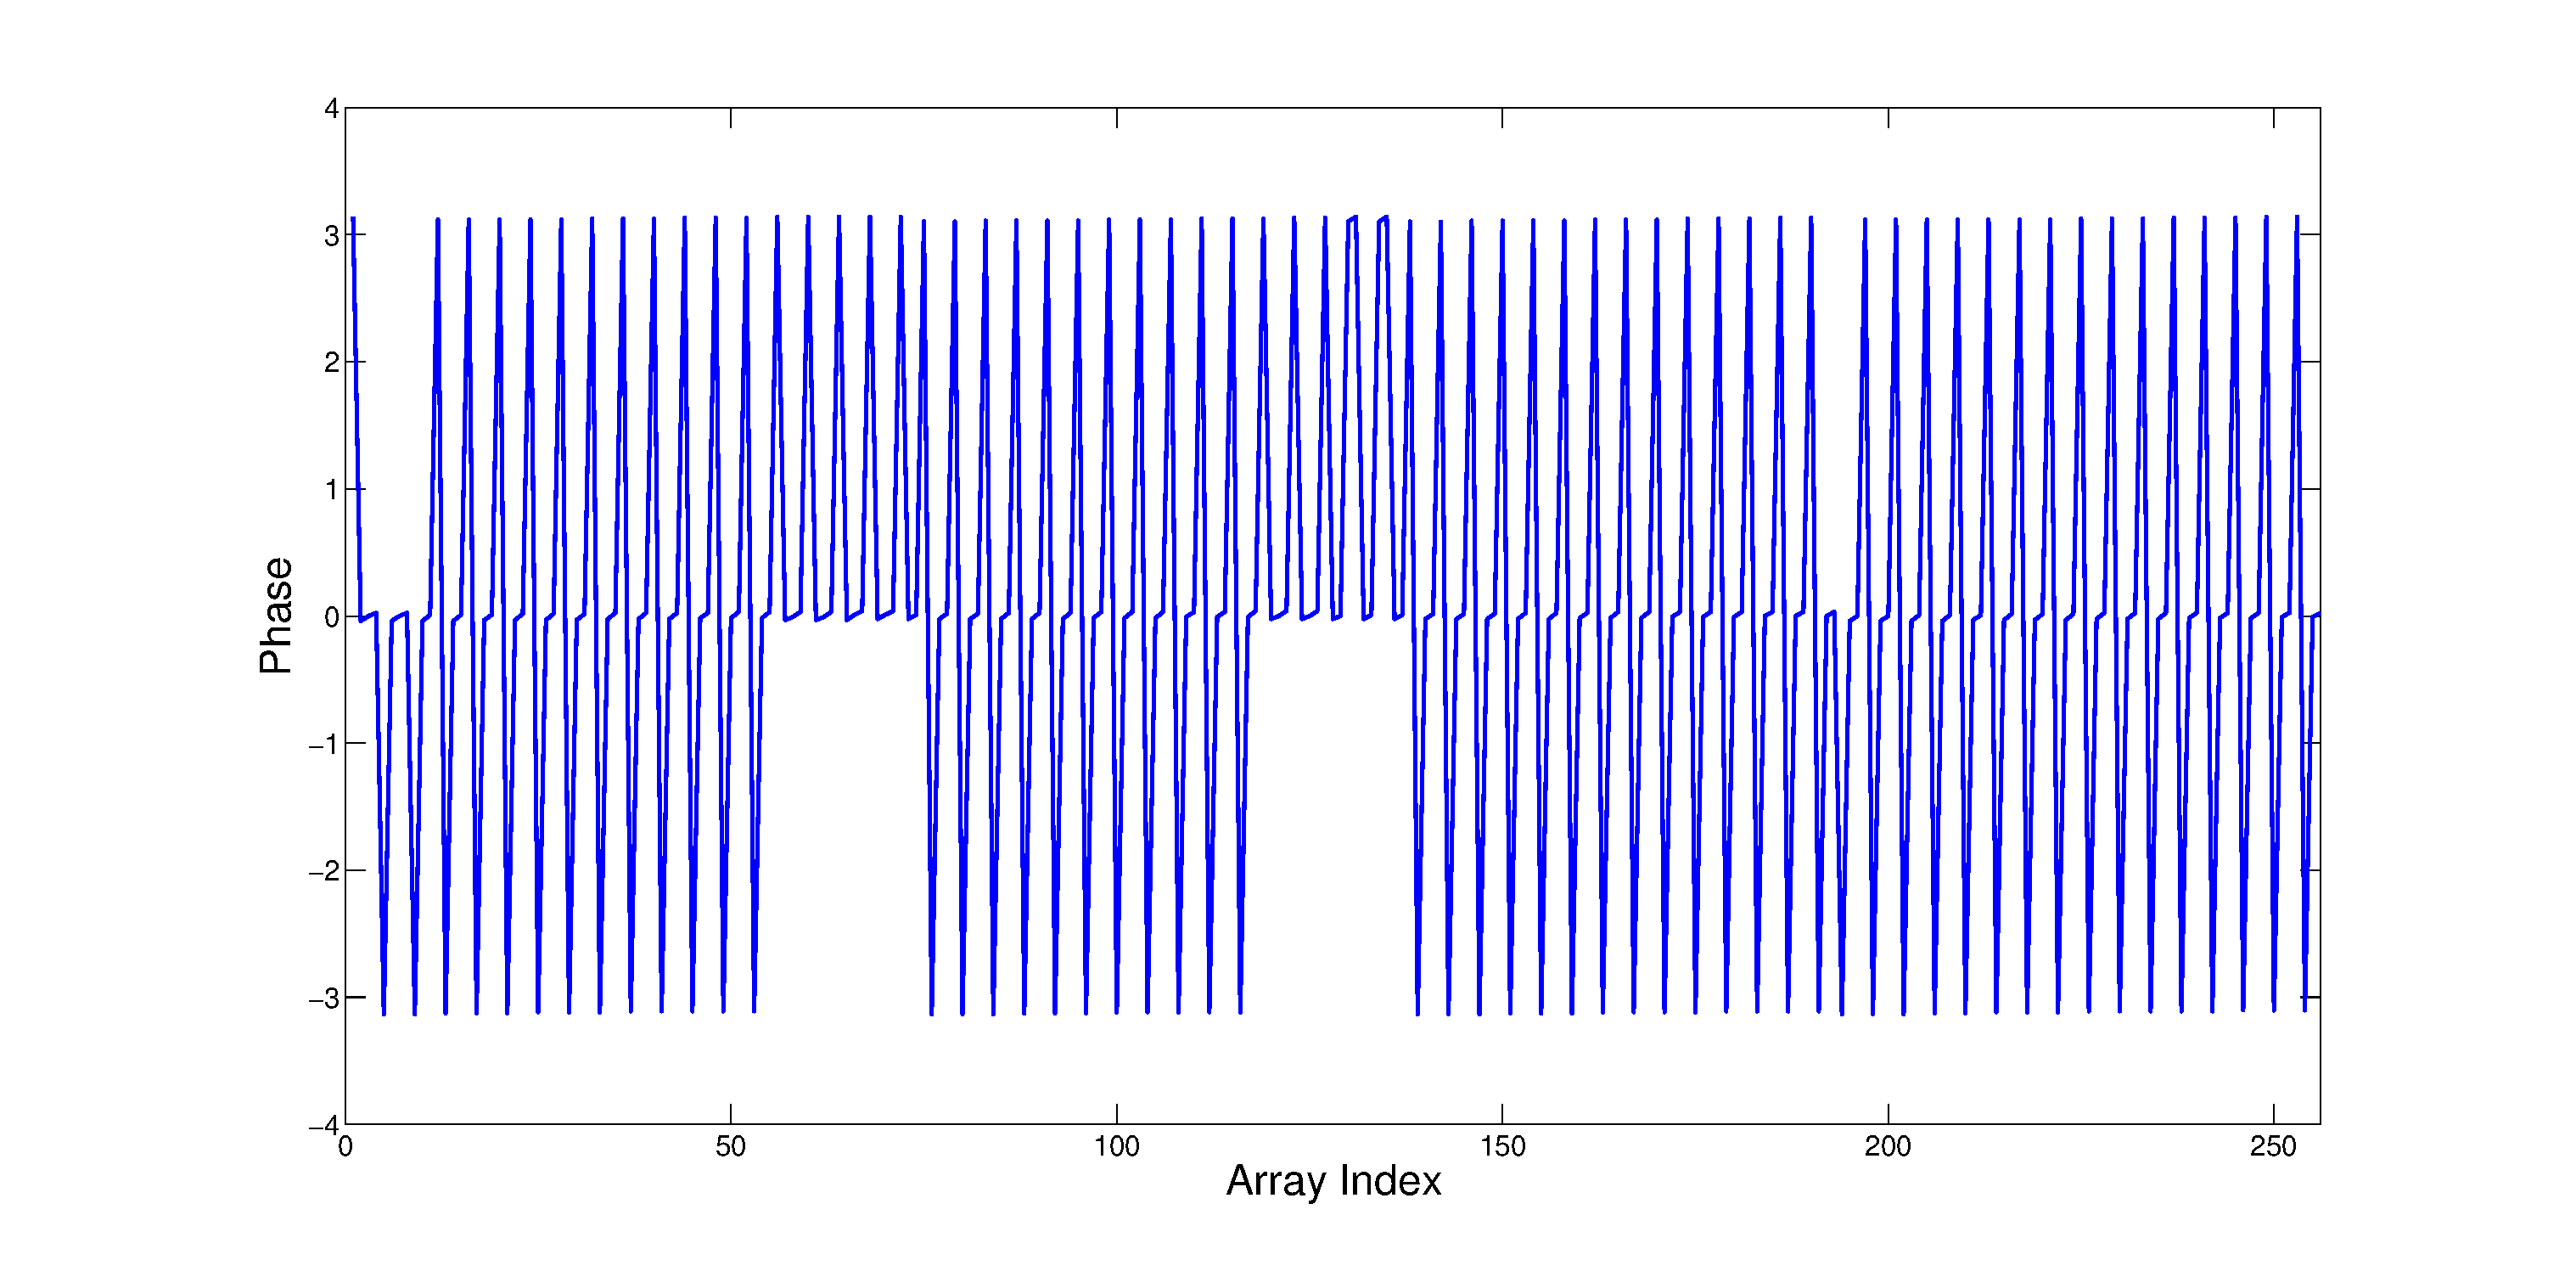
\includegraphics[width =\textwidth, keepaspectratio]{./Figures/AVR_FFT_Dirac_Complex_Phase.eps} }
\caption{Output phase and magnitude of the complex output from AVR fast Fourier transform of a Dirac function}
\label{fig:AVR:FFT:Dirac:Output}
\end{figure}

\begin{figure}
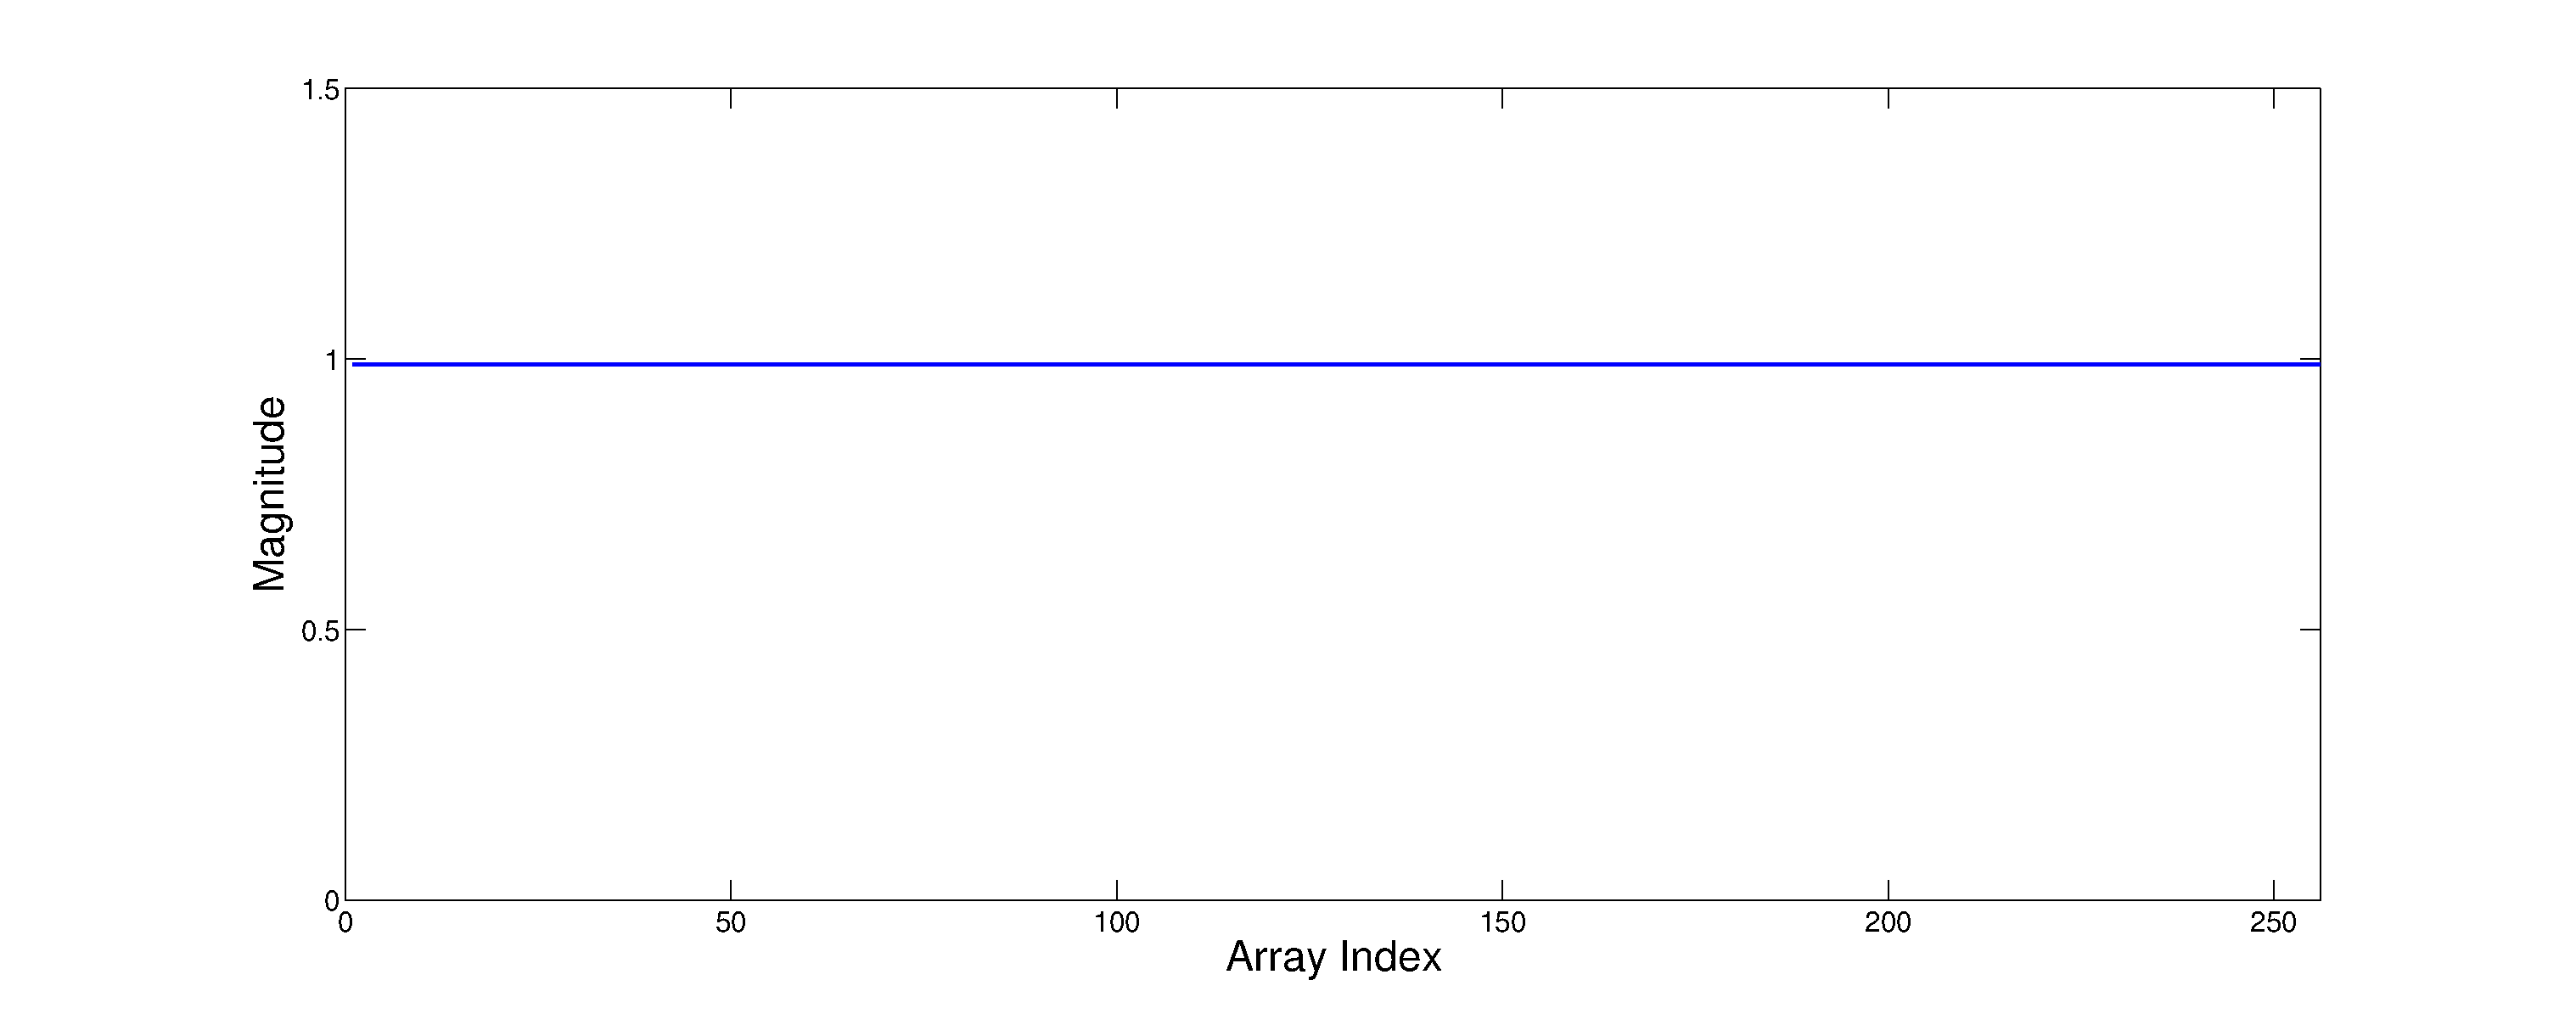
\includegraphics[width=\textwidth]{./Figures/AVR_FFT_Dirac_Mag.eps}
\caption{Magnitude calculated by the AVR of the Fourier transform of a Dirac function}
\label{fig:AVR:FFT:Dirac:Mag}
\end{figure}

\begin{figure}
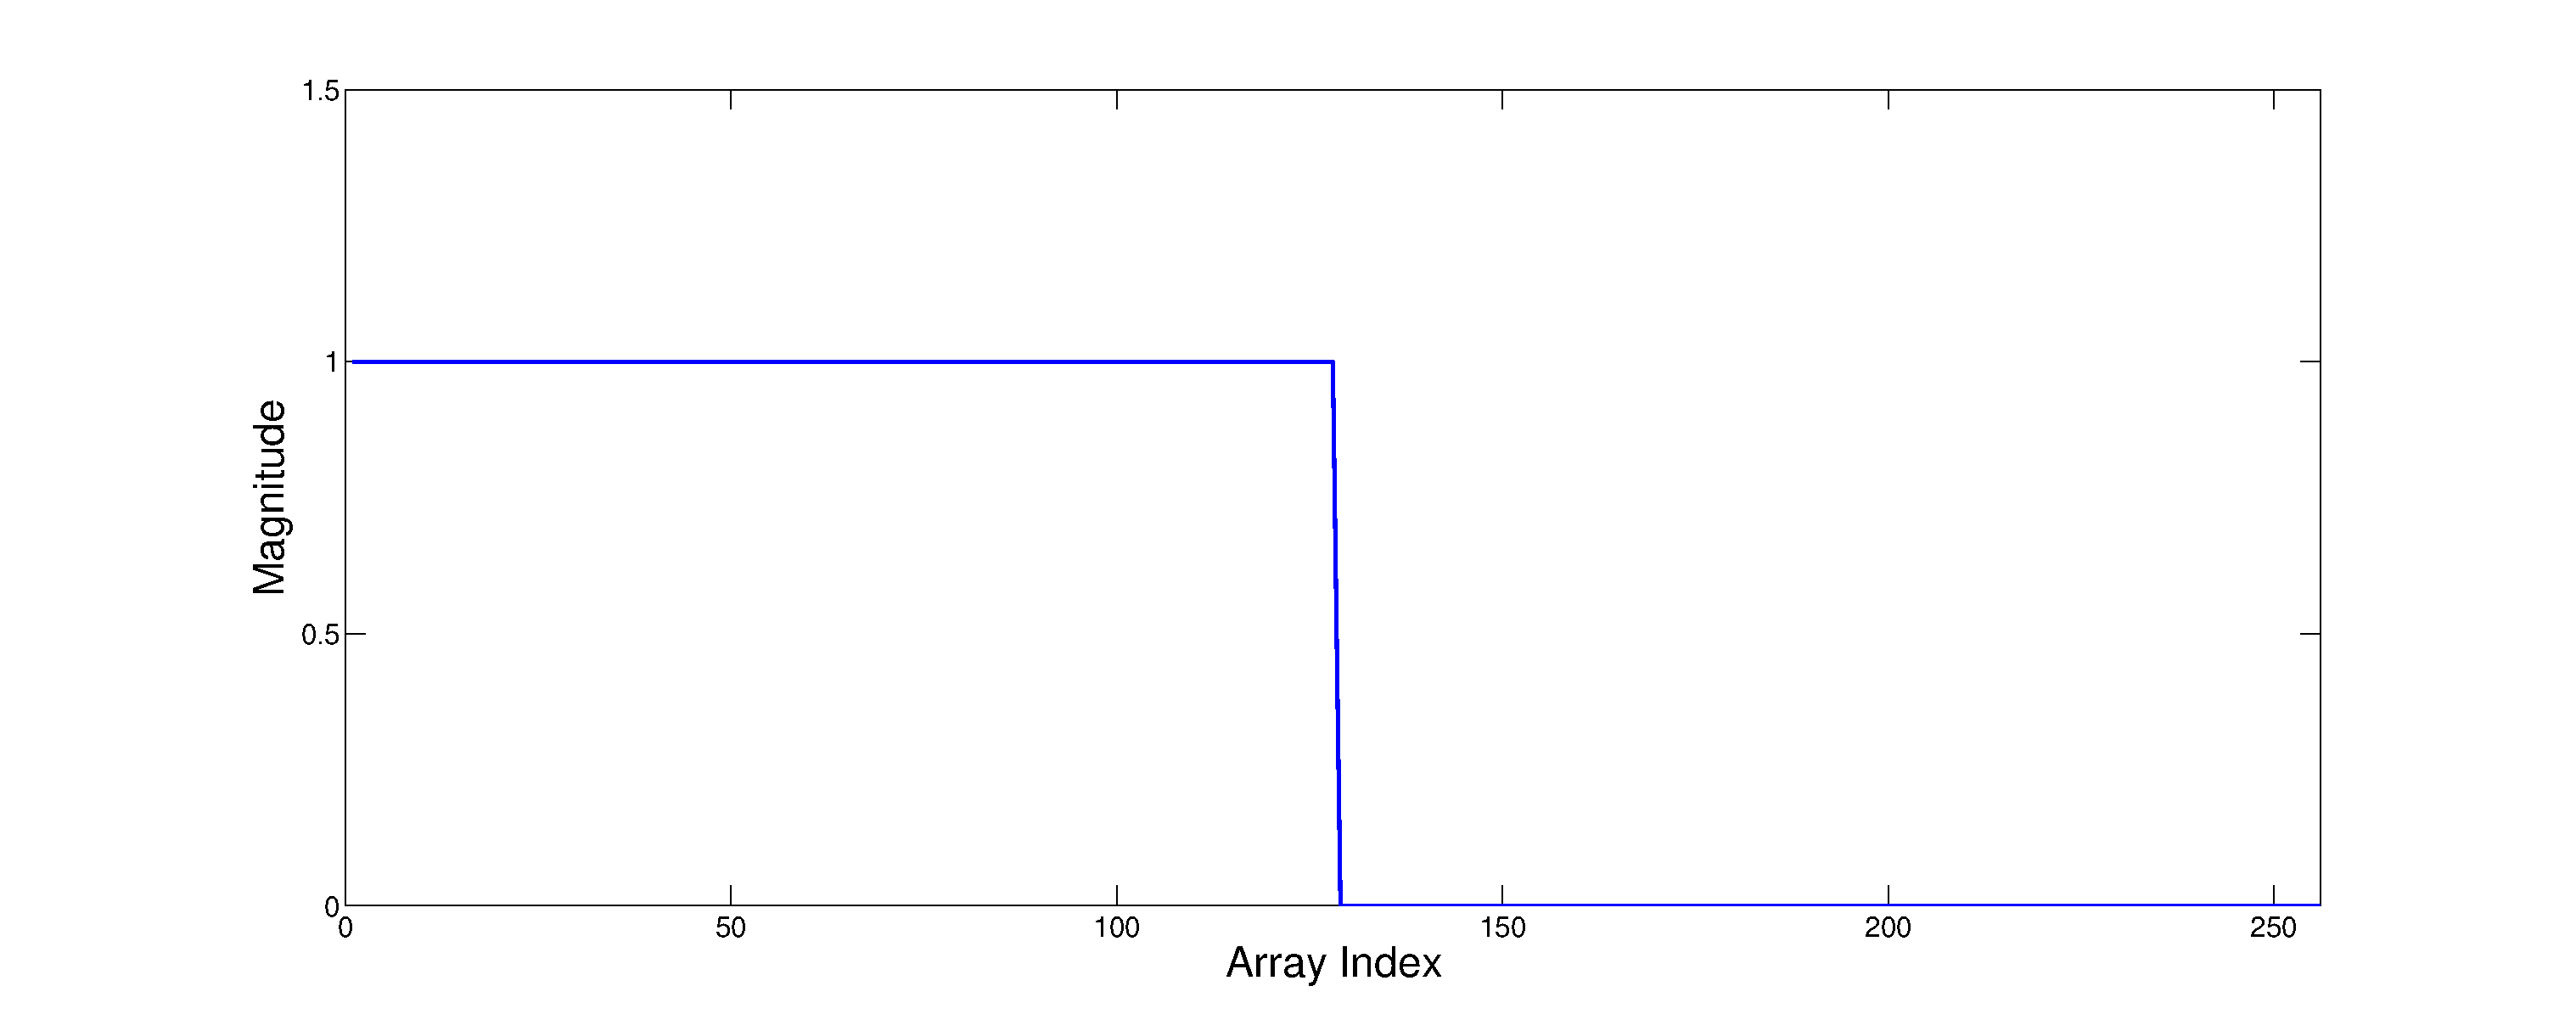
\includegraphics[width=\textwidth]{./Figures/AVR_FFT_Square_Input.eps}
\caption{Input rectangular pulse for AVR fast Fourier transform}
\label{fig:AVR:FFT:Square:Input}
\end{figure}
\begin{figure}
\subfigure[Magnitude of the complex output from the AVR]{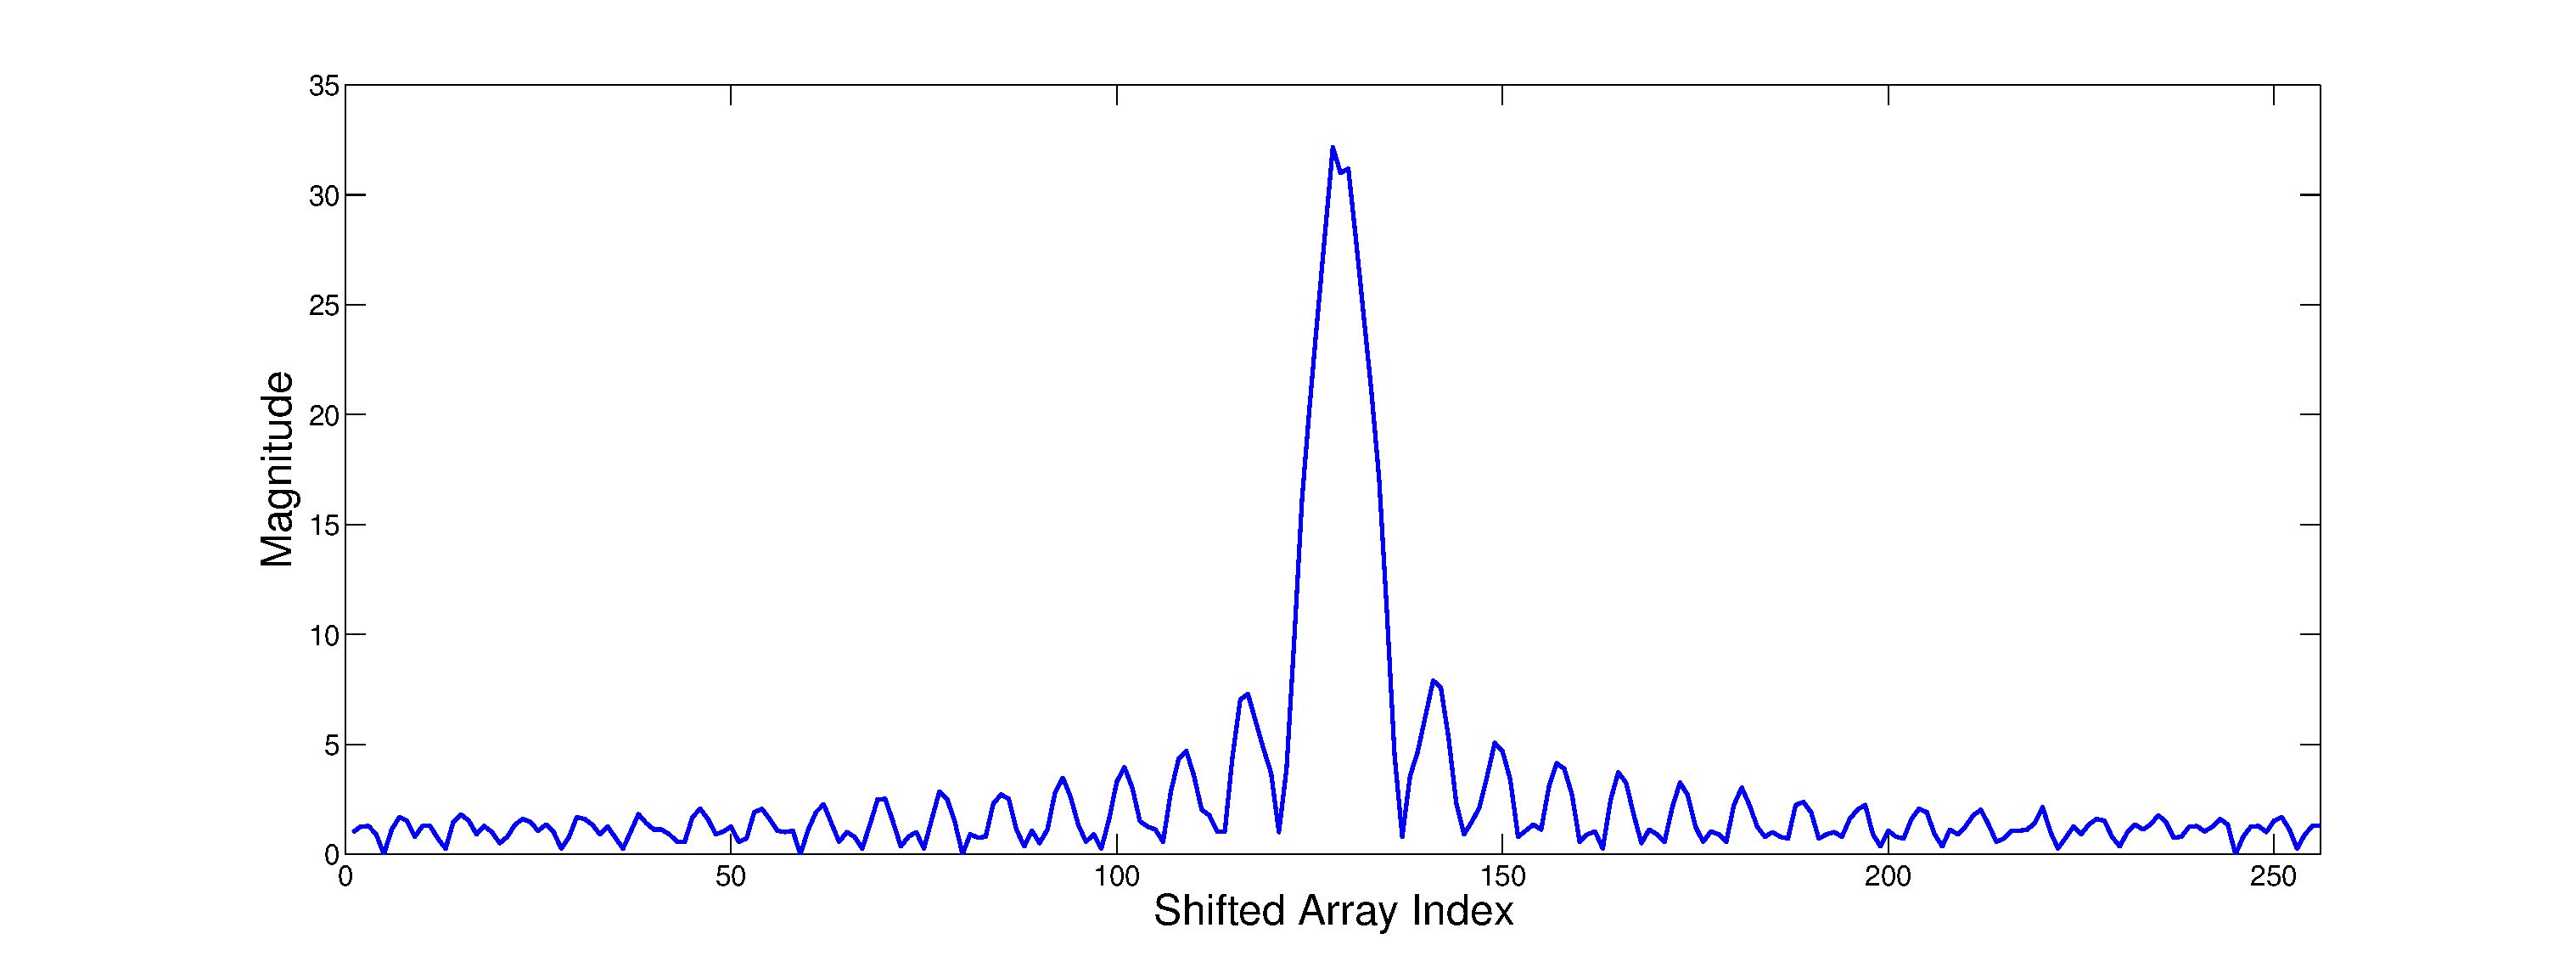
\includegraphics[width =\textwidth, keepaspectratio]{./Figures/AVR_FFT_Square_Complex_Mag.eps} }
\subfigure[Phase of the complex output from the AVR]{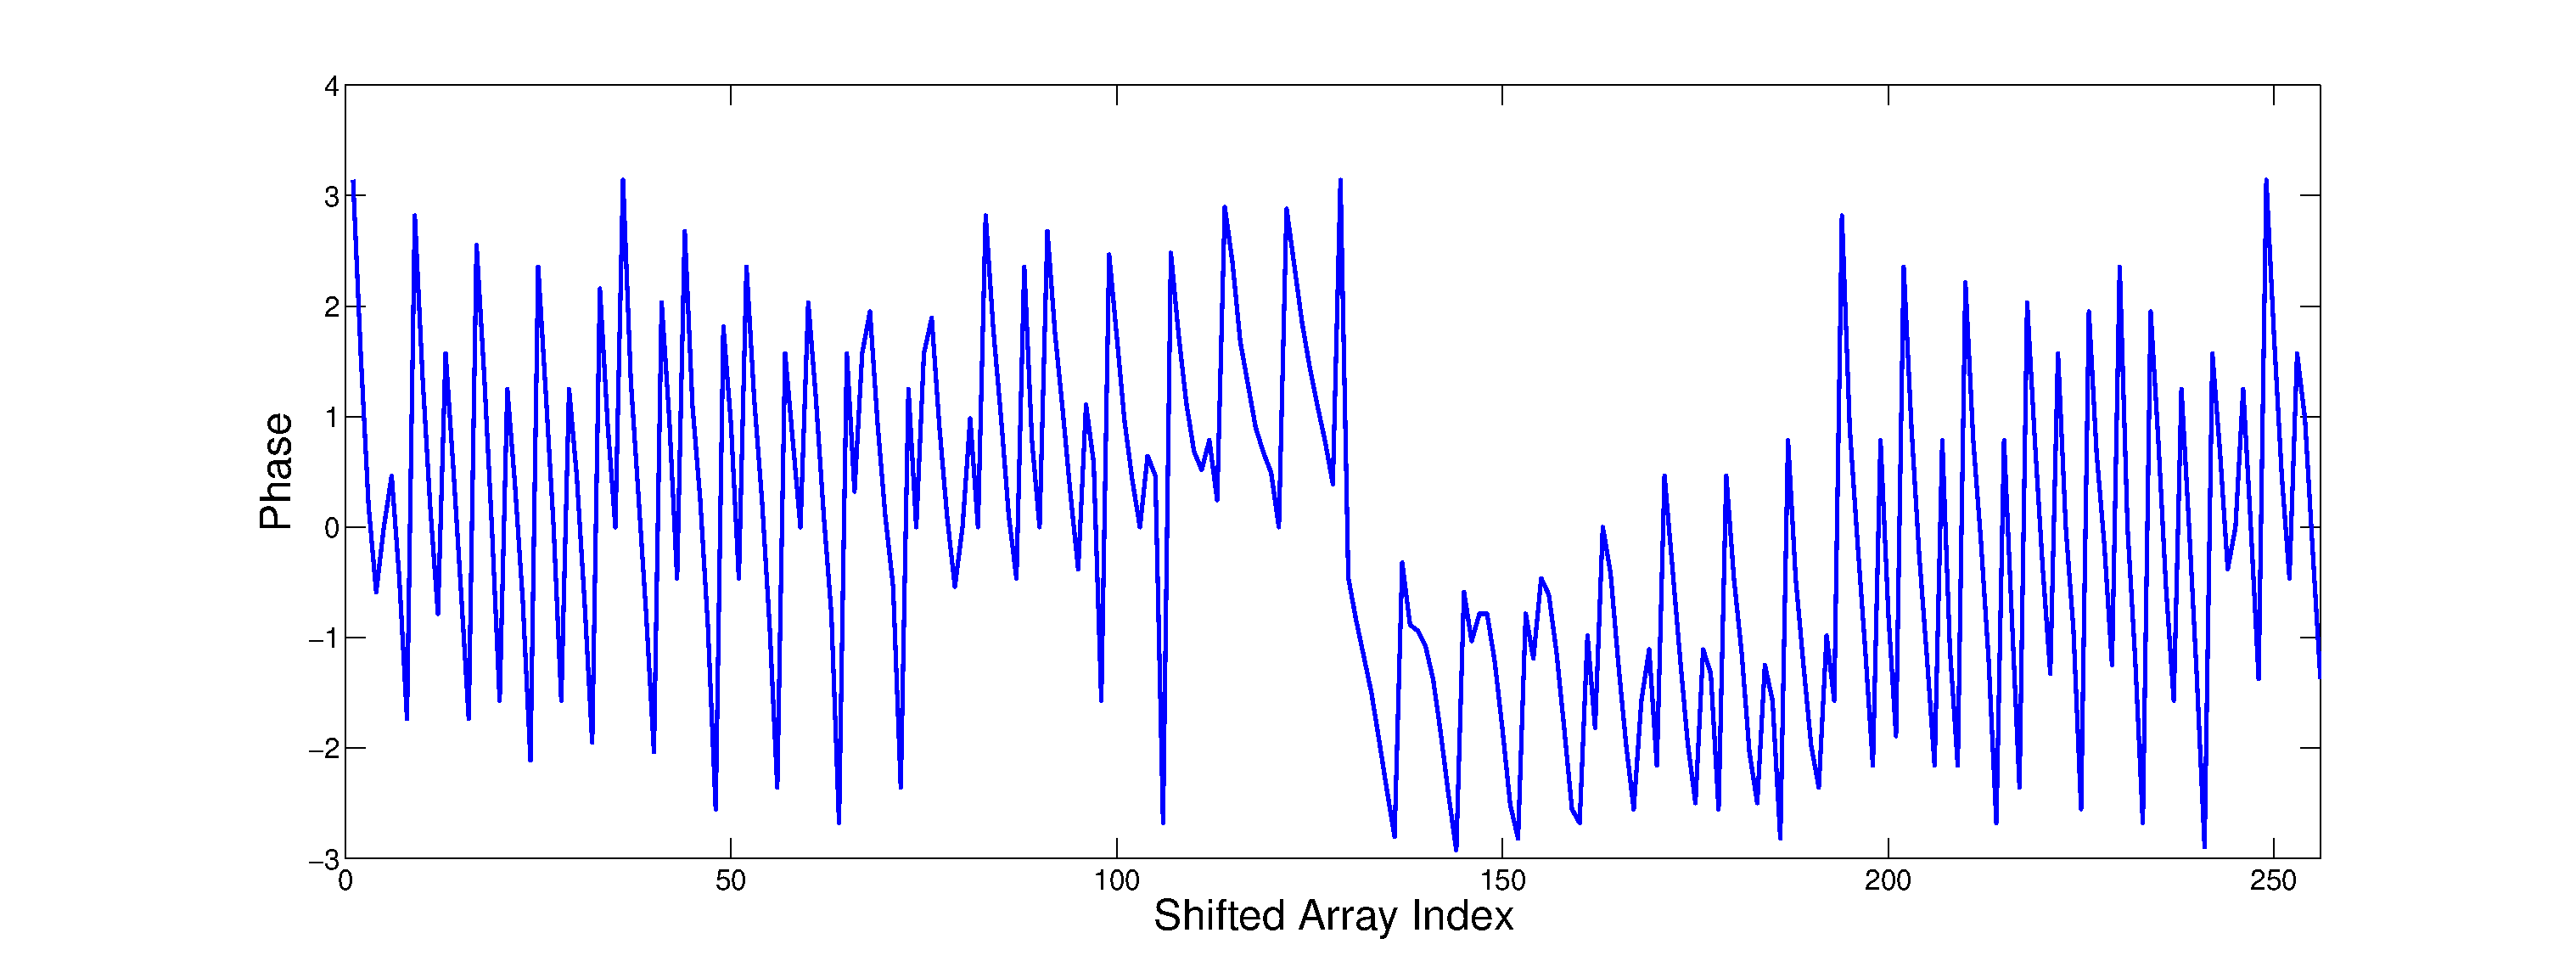
\includegraphics[width =\textwidth, keepaspectratio]{./Figures/AVR_FFT_Square_Complex_Phase.eps} }
\caption{Output phase and magnitude of the complex output from AVR fast Fourier transform of a rectangular pulse}
\label{fig:AVR:FFT:Square:Output}
\end{figure}
\begin{figure}
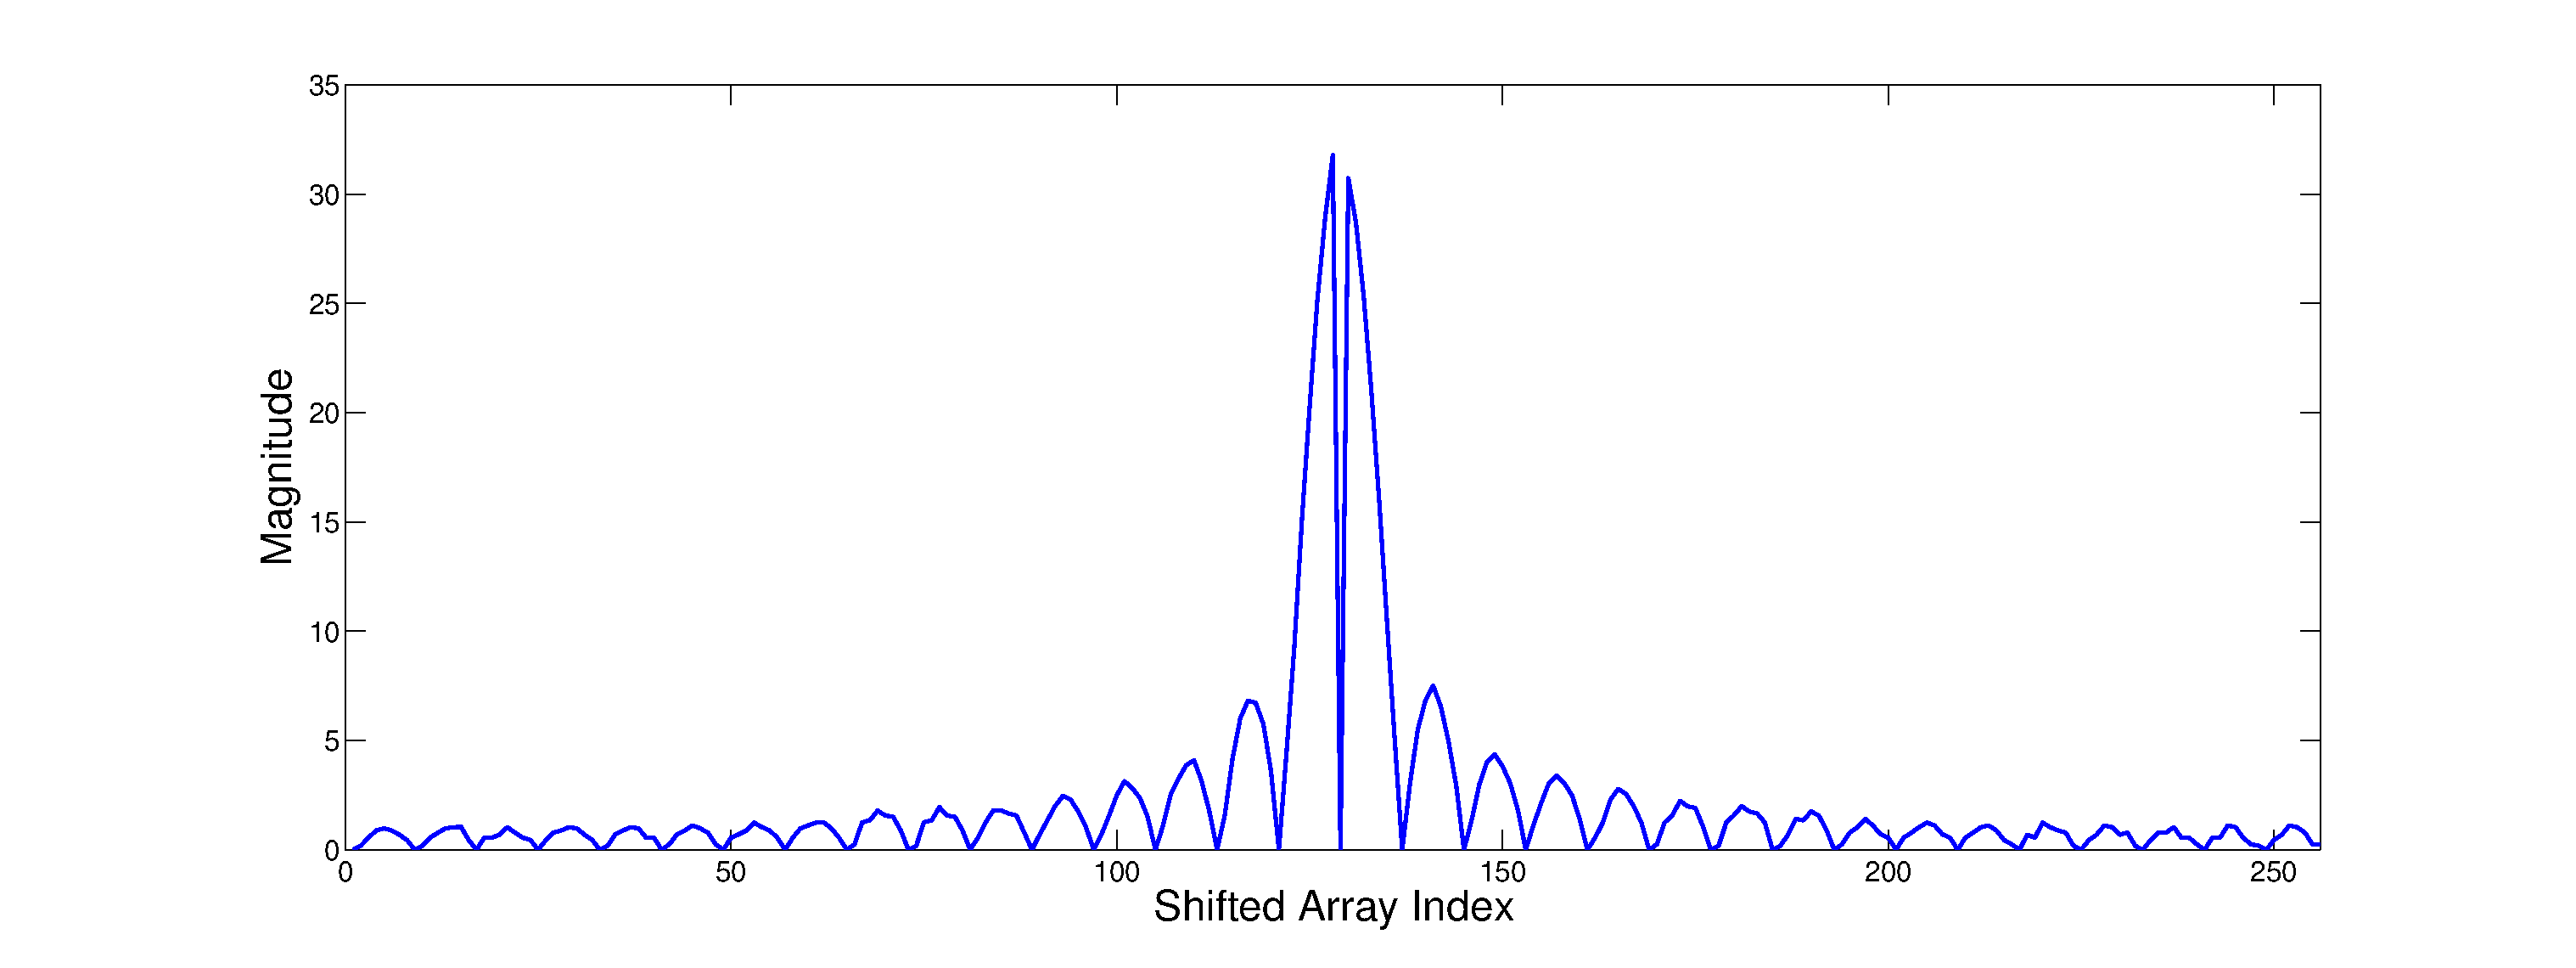
\includegraphics[width=\textwidth]{./Figures/AVR_FFT_Square_Mag.eps}
\caption{Magnitude calculated by the AVR of the Fourier transform of a rectangular pulse}
\label{fig:AVR:FFT:Square:Mag}
\end{figure}

\subsubsection{2D FFT Test}

Two test signals were used to test the 2D FFT on the AVR, a Dirac signal and a square wave, seen in Figures \ref{fg:Dirac2D:Signal} and \ref{fg:Square2D:Signal}. The internal method on the AVR was not able to compute the magnitude due to the method scaling all the values down causing truncation errors. The complex Fourier transform was obtained, saved to the SD card in CSV format and viewed in MATLAB. All data were normalised to omit the effects of the fixed point notation and the data shifted so that frequency 0 was in the centre. These tests were done with a $64\times64$ 2D data as with a $256 \times 256$ array the AVR runs out of internal RAM to calculate the transform. 
\inote{I would like to get this to work by the end but not vital.}

The result of the Dirac test is shown in Figure \ref{fig:AVR:FFT2:Dirac}. A similar error is found in the magnitude, but the spectrum is generally flat with a small amount of ripple as seen with the 1D FFT in Figure \ref{fig:AVR:FFT:Dirac:Mag}. The phase has similar issues as the 1D FFT. However, there appears to be the correct pattern with the 2D phase, but rotated about $45^{\circ}$. This is also the case with the square wave test. The magnitude in Figure \ref{fig:AVR:FFT2:Square:Mag} is very similar, with a distinct peak in the centre (frequency 0) and a sinc function extending vertically and horizontally from this. Again, the phase (Figure \ref{fig:AVR:FFT2:Square:Phase}) seems to differ a lot from the expected result in Figure \ref{fg:Square2D:Phase}. 
\begin{figure}
\subfigure[Normalised magnitude\label{fig:AVR:FFT2:Dirac:Mag}]{
\includegraphics[width=\textwidth / 2]{Figures/AVR_FFT2_Dirac_Mag.jpg}}
\subfigure[Phase \label{fig:AVR:FFT2:Dirac:Phase}]{
\includegraphics[width=\textwidth /2]{Figures/AVR_FFT2_Dirac_Phase.jpg}}
\caption{Images of the phase and magnitude of the complex data returned from the 2D FFT on the AVR of a 2D Dirac function}
\label{fig:AVR:FFT2:Dirac}
\end{figure}

\begin{figure}
\subfigure[Normalised magnitude\label{fig:AVR:FFT2:Square:Mag}]{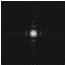
\includegraphics[width=\textwidth / 2]{Figures/AVR_FFT2_Square_Mag.jpg}}
\subfigure[Phase\label{fig:AVR:FFT2:Square:Phase}]{\includegraphics[width=\textwidth / 2]{Figures/AVR_FFT2_Square_Phase.jpg}}
\caption{Images of the phase and magnitude of the complex data returned from the 2D FFT on the AVR of a 2D square function}
\label{fig:AVR:FFT2:Square}
\end{figure}
\subsection{Conclusion}
The transforms are calculated in real time with a 16MHz clock source. Table \ref{table:FFTSize_Time} shows the number of clock cycles taken to calculate the relevant sized transform. A $64 \times 64$ transform takes $39ms$ to compute with a 16MHz clock. This could be reduced by increasing the internal clock speed on the AVR, potentially taking it up to 33MHz, and therefore halving the time to compute. A $64px \times 64px$ image, however, is not practical for the application. Larger transforms can be done, but further development is required to utilise the external RAM more efficiently.%more effort needs to be taken and the external RAM could be utilised more effectively.

\begin{table}
\centering
\caption{Number of clock cycles taken to calculate the transform of 64 or 256 long data set}
\label{table:FFTSize_Time}
\begin{tabular}{ccc} \toprule
 	& \multicolumn{2}{c}{ \textbf{Size of FFT Data} } \\ \cmidrule{2-3}
	& 	\textbf{64} 		& 	\textbf{256} \\ \toprule
1D 	&	5019 	& 	23599		\\ \midrule
2D 	& 	618168 	& 	- 	\\ \bottomrule
\end{tabular}
\end{table}



\inote{Show results of actual photo being transformed, need 2D 256 FFT working before}
\inote{Maybe IFFT it too to find total errors in algorithm?}
%\section{Low Level Vision Algorithms}
%\subsection{Noise Reduction}
%\inote{Why}
%Noise exists in all signals. Two noise sources for the camera image is random noise in the sensor, and quantisation noise. It generates a compromise between noise and resolution that has to be made. Large amounts of noise reduction will blur edges and therefore reduce the quality of the image and make it harder to match. This section will investigate some noise reduction methods, and test if the application of them increases the reliability of matching using the Normalised Cross Correlation method discussed in section \ref{Section:NCC}. 
%\inote{Theory}
%\inote{Examples}
%\inote{Does it improve the reliability of matching? Vary noise amount in images? and test}
%\subsection{Edge Detection}
%\inote{Why}
%\inote{Theory}
%\inote{Examples}
%\inote{Does it improve the reliability of matching?}

%%% ----------------------------------------------------------------
%% Results.tex
%% ---------------------------------------------------------------- 
\chapter{Results} \label{Chapter:Results}

\inote{A full test of the system I have got}
\inote{Summary of good and bad WITH EVIDENCE}
%% ----------------------------------------------------------------
%% Conclusions.tex
%% ---------------------------------------------------------------- 
\chapter{Conclusions and Further Work} \label{Chapter: Conclusions}
%\section{Conclusion}

%\inote{What I have accomplished}
This work has led to a tested device which is mobile and has the capability to perform stereoscopic image processing. The system has the following parts:

\begin{enumerate}
\item Motor driving
\item Stereoscopic Cameras
\item SD Card memory
\item SRAM
\item Image Processing
\end{enumerate} 

The motor system is a simple, cheap method to move distances with reasonable accuracy. A better controller would allow variable speed and speed matching between motors. The system was shown to work to $4.5\%$ accuracy over a $300mm$ distance.

A full image can be read from a camera and stored on an SD card in a FAT32 file system. This gives the ability of removable memory that can be viewed on a computer to see any internal logs. Images are stored in QVGA format (320 by 240 pixels) as a bitmap image. 

An additional 4MB of SRAM memory is available to use on the robot allowing for large data arrays of the images to be kept in fast access RAM. The RAM is direct memory accessed so operation is almost seamless from internal memory.

Multiple comparison algorithms have been investigated and compared using the same test images. It was clear that, although at a necessity of more computations, the normalised cross correlation is the best with regard to overall reliability. 

The Fourier transform was also investigated and implemented. The system allows for a $2 \times 2$ array of a square image with dimensions of $2^{2n}\; $ where $n \in \mathbb{N}$ and is limited by RAM space and time. The transform is speed optimised and in tests proved to be fairly accurate. 

Range finding equations were then derived, which use the characteristics of the camera and the separation distance between them. %They have also been tested using MATLAB and images that have been rendered where all the distances are known and exact.

All aspects implemented on the robot have been shown to be functional. A faster processor would have been a good idea to use for image processing, but this could have developed other problems with the PCB. The Raspberry Pi or Steve Gunn's \textit{`L'Imperatrice'}, which both run a Linux operating system, would have been a good choice to remove the need for as much hardware design and existing image processing libraries could have been utilised to gain more functionality in the time. 

Though the robots original application wasn't achieved, the end device is a base for a stereoscopic application. The system is a tested platform for future applications to be implemented on and additions can be made using the spare pins and bus connections on the PCB headers. 

The system could be used in future projects to develop more functionality. Wireless communications could be added to the system to allow a connection to the computer and search algorithms can be implemented alongside distance calculations to make the robot aware of its surroundings. 
%\inote{What could be changed to make it better}
%\inote{Suggestions for further work}

\appendix
%% ----------------------------------------------------------------
%% AppendixD.tex
%% ---------------------------------------------------------------- 
\chapter{Gantt Charts} \label{Chapter:AppendixD:Gannt}

\begin{figure}
\centering
\includegraphics[angle = 90,height=\textheight]{Figures/Gantt.pdf} 
\caption{Gantt Chart of how time was decided to be spent at the beginning of the project}
\label{fig:Gantt:1}
\end{figure}
\clearpage
\begin{figure}
\centering
\includegraphics[angle = 90, height=\textheight]{Figures/Gantt2.pdf} 
\caption{Gantt Chart of how time during term two was decided to be spent after interim report hand-in}
\label{fig:Gantt:2}
\end{figure}

\begin{figure}
\centering
\includegraphics[angle = 90, height=\textheight]{Figures/Gantt3.pdf} 
\caption{Gantt Chart of how time was actually spent throughout the project}
\label{fig:Gantt:3}
\end{figure}
%% ----------------------------------------------------------------
%% AppendixA.tex Circuit Diagrams
%% ---------------------------------------------------------------- 
\chapter{Circuit Diagrams} \label{Chapter:AppendixA:CircuitDiagrams}
\section{OV7670 Breakout Board Schematic}\label{sch:OV7670}
\begin{figure}[ht!]
\centering
\includegraphics[angle=90,width=\textwidth,height=\textheight-10cm,keepaspectratio]{Figures/OV7670_Schematic.jpg} 
\caption{The circuit diagram for the OV7670 breakout board}
\label{OV7670_Schematic}

\end{figure}
\clearpage
\section{Il Matto and Dual Camera Schematic}\label{sch:IlMatto:Cameras}
\begin{figure}[ht!]
\centering
\includegraphics[angle = 90, width=\textwidth,height=\textheight,keepaspectratio]{Figures/IlMattoCamera_CircuitDiagram.png} 
\caption{The circuit diagram for Dual Cameras using the Il Matto Board}
\label{sch:DualCam_Schematic}
\end{figure}
\clearpage

\section{The Columbus Circuit Diagram} \label{sch:Columbus:CircuitDiagram}
\begin{figure}[ht!]
\centering
\includegraphics[angle = 90, width=\textwidth,height=\textheight,keepaspectratio]{./Figures/ColumbusCircuitPage1.png}
\caption{The Columbus Circuit Diagram Page 1}
\label{sch:Columbus_Schematic:1}
\end{figure}

\begin{figure}[ht!]
\centering
\includegraphics[angle = 90, width=\textwidth,height=\textheight,keepaspectratio]{./Figures/ColumbusCircuitPage2.png}
\caption{The Columbus Circuit Diagram Page 2}
\label{sch:Columbus_Schematic:2}
\end{figure}

\begin{figure}[ht!]
\centering
\includegraphics[angle = 90, width=\textwidth,height=\textheight,keepaspectratio]{./Figures/ColumbusCircuitPage3.png}
\caption{The Columbus Circuit Diagram Page 3}
\label{sch:Columbus_Schematic:3}
\end{figure}

\begin{figure}[ht!]
\centering
\includegraphics[angle = 90, width=\textwidth,height=\textheight,keepaspectratio]{./Figures/ColumbusCircuitPage4.png}
\caption{The Columbus Circuit Diagram Page 4}
\label{sch:Columbus_Schematic:4}
\end{figure}

\begin{figure}[ht!]
\centering
\includegraphics[angle = 90, width=\textwidth,height=\textheight,keepaspectratio]{./Figures/ColumbusCircuitPage5.png}
\caption{The Columbus Circuit Diagram Page 5}
\label{sch:Columbus_Schematic:5}
\end{figure}

\begin{figure}[ht!]
\centering
\includegraphics[angle = 90, width=\textwidth,height=\textheight,keepaspectratio]{./Figures/ColumbusCircuitPage6.png}
\caption{The Columbus Circuit Diagram Page 6}
\label{sch:Columbus_Schematic:6}
\end{figure}


%% ----------------------------------------------------------------
%% AppendixA.tex Circuit Diagrams
%% ---------------------------------------------------------------- 
\chapter{PCB Design} \label{Appendix:PCB}
\section{PCB Top Side}
\begin{figure}[ht!]
\centering
\includegraphics[angle=90,width=\textwidth,height=\textheight-5cm,keepaspectratio]{Figures/PCB_Top.pdf} 
\caption{The top side of the CAD design of the PCB (Ground plane omitted)}
\label{fig:PCB:Eagle:Top}
\end{figure}
\clearpage
\section{PCB Layer 2}
\begin{figure}[ht!]
\centering
\includegraphics[angle=90,width=\textwidth,height=\textheight-5cm,keepaspectratio]{Figures/PCB_3v3.pdf} 
\caption{Layer 2 of the CAD design of the PCB}
\label{fig:PCB:Eagle:Bottom}
\end{figure}
\clearpage
\section{PCB Layer 3}
\begin{figure}[ht!]
\centering
\includegraphics[angle=90,width=\textwidth,height=\textheight-5cm,keepaspectratio]{Figures/PCB_GND.pdf} 
\caption{Layer 3 of the CAD design of the PCB}
\label{fig:PCB:Eagle:Bottom}
\end{figure}
\clearpage
\section{PCB Bottom Side}
\begin{figure}[ht!]
\centering
\includegraphics[angle=90,width=\textwidth,height=\textheight-5cm,keepaspectratio]{Figures/PCB_Bottom.pdf} 
\caption{The bottom side of the CAD design of the PCB (Ground plane omitted)}
\label{fig:PCB:Eagle:Bottom}
\end{figure}
\clearpage
%% ----------------------------------------------------------------
%% AppendixA.tex Circuit Diagrams
%% ---------------------------------------------------------------- 
\chapter{Costings and Components} \label{Appendix:Costings}

\begin{table}
\centering
\caption{A table of all components used and their costs.}
\label{table:Costings}
\begin{tabular}{|c|p{2cm}|c|c|c|} \hline
Component	&	Cost per unit (\pounds)	& Quantity 	&	Cost (\pounds)		&	Source		\\ \hline
PCB			&	205						&	1		&	205					&	PCBCart		\\
Capactiors	&	0.155 					& 	43		& 	6.67 				& 	Farnell 	\\
Clock 		& 	1.48					& 	1		&	1.48 				& 	Farnell		\\
Diode		&	0.48					&	1		&	0.48				&	Farnell 	\\
Headers		&	0.51 					&	5		&	2.55				&	Farnell 	\\
I2C Mux PCA9542A &	0.81				&	1		&	0.81				&	Farnell		\\
LEDs 		&	0.158					&	7		& 	1.11 				&	Farnell		\\
Micro SD Card &	4						&	1		&	4.00 				&	Amazon 		\\
Micro SD Card Connector & 2.04			&	1		&	2.04				&	Farnell		\\
AT32UC3C0512C	&15.39					&	1		&	15.39				&	Farnell		\\
TB6593FNG 	&	1.07 					&	2 		&	2.14 				&	Farnell 	\\
Motors  	&	0.42					&	2		&	0.84				&	Rapid 		\\
TCRT1010	& 	0.94 					&	2		&	1.88 				&	Farnell 	\\
OV7670		&	17						&	2		&	34.00				& 				\\
Potentiometer	&	0.43				&	2		&	0.86				&	Farnell 	\\
Resistors	&	0.066 					& 	46		&	3.04 				&	Farnell 	\\
MT48LC4M16A2P	& 3.24  				& 	1		&	3.24 				&	Farnell		\\
Switch		&	0.45					&	1		&	0.45				&	Farnell 	\\
USB Socket	&	0.84 					&	1		& 	0.84 				&	Farnell 	\\
LM1117MP	&	1.03					&	1		&	1.03	 			&	Farnell		\\ \hline \cline{3-4}
\multicolumn{2}{c|}{ }					& Total Cost  & \pounds 287.84		&	\multicolumn{1}{|c}{ }			\\ \cline{3-4}
\end{tabular}
\end{table}


\begin{table}
\caption{All components and their values (if applicable)}
\label{table:Components}
\begin{tabular}{|p{7cm}|p{5cm}|}\hline
Compnent(s)		&	Value \\ \hline
IC1				&	AT32UC3C0512C \\
IC2 & PCA9542A \\
IC3 & MT48LC4M16A2 \\
IC4, IC5 & TB6593FNG \\
Q1, Q2 & OV7670 \\
Q3	&	LM1117MP-3.3\\
Q4, Q5	& TCRT1010 \\
S1				&	Tactile Switch \\
R15, R16 & $10k\Omega$ Potentiometer\\
R17, R18, R19, R20, R21, R22, R23, R24, R25, R26, R27, R28, R29, R30, R31, R32, R33, R37, R38, R39, R40 & $68\Omega $ \\
R11, R13 & $150\Omega$ \\
R44, R45, R46, R47, R48, R49, R50	& $330\Omega$ \\
R2, R3, R4, R5, R6, R7, R8, R9, R10,  R34, R35 & $4K7\Omega$ \\
R1, R12, R14	& $10k\Omega$ \\
R36, R41	& $100k\Omega$ \\

C1, C2	&	$22pF$ \\
C6 & $1nF$ \\
C9, C11, C13, C15, C17, C20, C22, C25, C28, C30, C43 & $33Nf$ \\
C7, C12, C14, C16, C18, C19, C21, C24, C27, C29, C31, C32, C33, C34, C36, C38, C39, C42	&	$100nF$ \\
C5	&	$2.2\mu F$ \\
C8, C10, C23, C26  & $4.7\mu F $ \\
C3, C4, C35, C37, C40, C41 &	$10\mu F$ \\

D1 & GF1A - Rectifier Diode \\
J1, J2, J3, J4, J5, J6, J7, J8, J9 & 0.1'' header \\
LED2, LED3, LED4, LED5, LED6, Motor LED, Power LED	&	1206 LED \\ 
X2 & Micro SD Card Socket \\ \hline
\end{tabular}
\end{table}
%% ----------------------------------------------------------------
%% AppendixC.tex
%% ---------------------------------------------------------------- 
\chapter{Contents of Design Archive} \label{Appendix:Contents}
\begin{itemize}
%\item Contents.txt
%\item encc\_matlab.zip
%\item Harris.zip
%\item README
%\item stereo\_example.zip
%\item TcfTransactionLog.csv
%\item texput.log
\item CircuitDiagrams - Contains the EAGLE circuit diagram and PCB files
\begin{itemize}
\item Project - Final design files of the PCB
\item IlMatDual - EAGLE Schematic for \textit{Il Matto} and Dual Camera design
%\begin{itemize}
%\item eagle.epf
%\item project.bcl.pdf
%\item project.brd
%\item project.pdf
%\item project.pro
%\item project.sch
%\item project.tcl.pdf
%\end{itemize}
\end{itemize}
\item Code - Contains all code
\begin{itemize}
\item AnalogueComparator - Code used to investigate the Analogue Comparators on the UC3C
\item Camera\_TFT - Program for streaming the camera feed to the TFT screen with the \textit{Il Matto}
\item ColumbusTest - The test program for the PCB
\item DualCamera\_UI - Code for the ATMega168 used in the Prototype
\item DualOV7670 - Code for the ATMega644P used in the Prototype
\item FatFS - FatFS Code for use on the Il Matto 
\item MotorDriver - Code written during testing of the Motor driver system
\item OV7670+AVR+TFT-Jian - Original Camera Code used
\item OV7670seblov - Camera code to send image to PC
\item OV7670\_FATFS - Camera Code for Il Matto to store images to SD Card
\item PhotoViewer - C\# Application to receive a photo over UART
\item SDCard - An attempt using Petite Fat
\item SDTest - Example code using the Il Matto and Petite Fat library supplied by Steve Gunn
\item The\_Columbus - The final code used for the Robot
\end{itemize}
\item Documents - A collection of research and datasheets. 
%\begin{itemize}
%\item 0.3M Sensor OV7670.pdf
%\item AT32UC3.pdf
%\item ATmega644P.pdf
%\item Costings.xlsx
%\item EffectiveCornerMatching.pdf
%\item ExampleProjectWriteUp.pdf
%\item Iterative\_Image\_Registration.pdf
%\item lm1117.pdf
%\item MT48LC16M4A2.pdf
%\item PCA9542A.pdf
%\item PCBChanges.txt
%\item RegistationofStereoandTemporalImages.pdf
%\item research.txt
%\item SDRAM.pdf
%\item Stereoscopy\_(Mrovlje).pdf
%\item SzeliskiBook.pdf
%\item TB6593FNG.pdf
%\item tcrt1000.pdf
%\end{itemize}
\item Matlab - All \textsc{Matlab} Code used for prototyping
\begin{itemize}
\item archive - An archive of scripts of little relevance
\item Figures - *.fig files of \textsc{Matlab} generated Graphs for the Report
\item Images - A collection of images used for prototyping
\item Range\_Test\_Images - Images used for the Range Test
\end{itemize}
\item ProjectBrief - Project brief related files
\item Report - Report, and interim report, write up related files
\begin{itemize}
\item Figures - All figures used in the reports
\end{itemize}
\item SDCard - Files on the MicroSD card. 
\item Contents.txt - contents list of the directory
\item log.txt - Git commit log of the project
\end{itemize} 
        

%% ----------------------------------------------------------------
%% AppendixB.tex
%% ---------------------------------------------------------------- 
\chapter{Bitmap File Format} \label{Chapter:AppendixB:BMPFile}
\section{Bitmap File Format}
\begin{center}
\begin{longtable}{|p{2.5cm}|p{2.5cm}|p{4cm}|p{2cm}|p{2cm}|}
\caption{Format of a Bitmap file with values used, to write an image from the camera to an SD card} \label{tab:BMPFileFormat} \\

\hline Section	&	Field	&	Description					& Size (Bytes)	& Value (hex)\\ \hline
\endfirsthead

\multicolumn{3}{c}%
{{ \tablename\ \thetable{} -- continued from previous page}} \\
\hline Section	&	Field	&	Description					& Size (Bytes)	& Value (hex)\\ \hline 
\endhead

\hline \multicolumn{5}{|r|}{{Continued on next page}} \\ \hline
\endfoot

\hline \hline
\endlastfoot

Bitmap Header& Signature&	Declares the file is a Bitmap Image		& 2			& 424D\\
		&	File Size&	Size of the whole file including headers	& 4			& 36580200 (153654)\footnote{This is different to the 225kB stated in table \ref{ImageFormats} due to omitting many optional fields} \\ 
		&	Reserved&							&	 4	& 00000000 \\
		& 	Offset to Pixel Array & The address of the start of the pixel data from the beginning of the file & 4 & 36000000 \\
\hline
DIB (Device Independent Bitmap) Header & Size & Size of the DIB Header (dictates the version) & 4	&	7C000000 \\
	& 	Width	& Width of the image (320 pixels) & 4 	&	40010000 \\
	& 	Height	& Height of the image (240 pixels)	& 	4	& F0000000 \\
	& 	Planes	& Number of colour planes		& 2 & 0100 \\
	&	Bit Count & Number of bits per pixel & 2 & 1000 \\
	& 	Compression & Compression Being Used, RGB Bit Fields & 4 & 03 00 00 00 \\
	&	Image Size & Size of the image & 4 & 00 86 25 00 \\
	& 	X Resolution 	& Horizontal resolution in pixels per metre & 4 & 13 0B 00 00 \\
	& 	Y Resolution 	& Vertical resolution in pixels per metre & 4 & 13 0B 00 00 \\
	& 	Colours in Table & Number of colours in the colour table (not used) & 4 &  00 00 00 00\\
	&	Important Colours & 	Number of Important Colours (0 means all colours are important) & 4 & 00 00 00 00 \\
	& 	Red Mask 		& Bit mask of Red field 	& 4 & 00 F8 00 00 \\
	& 	Green Mask 		& Bit mask of Green field 	& 4 & E0 07 00 00 \\
	& 	Blue Mask 		& Bit mask of Blue field 	& 4 & 1F 00 00 00 \\
	& 	Alpha Mask 		& Bit mask of Alpha field 	& 4 & 00 00 00 00 \\
	& 	Colour Space Type & Colour Space of the DIB & 4 & 01 00 00 00 \\
	&	Colour Space Endpoints & Sets endpoints for colours within the bitmap (not used) &	36	& Whole Field = 0 \\
	& 	Gamma Red	&	Gamma Value of Red Field (not used) & 4 & 00 00 00 00 \\
	& 	Gamma Green&	Gamma Value of Green Field (not used) & 4 & 00 00 00 00 \\
	& 	Gamma Blue	&	Gamma Value of Blue Field (not used) & 4 & 00 00 00 00 \\
	&	Intent 	& 	Enum dictating the intent of the image (Picture) & 4 & 03 00 00 00 \\
	& 	ICC Profile Data & 	Offset from the file start to the ICC Colour Profile (Not Used) & 4 &  00 00 00 00 \\
	& ICC Profile Size & Size of the ICC Colour Profile (not used)	& 4 & 00 00 00 00 \\
	& Reserved & & 4 & 00 00 00 00 \\
\hline
Image Data Format & Each field contains all the pixel data& Padding is used to make the table width a multiple of 4 (Not always needed) & &\\
 Pix[0, h-1] 	& Pix[1, h-1] 	& \dots & Pix[w-1, h-1] & Padding \\
\vdots & \vdots & \vdots & \vdots & \vdots \\
 Pix[0, 1] 	& Pix[1, 1] 	& \dots & Pix[w-1, 1] & Padding \\
 Pix[0, 0] 	& Pix[1, 0] 	& \dots & Pix[w-1, 0] & Padding 
\end{longtable}
\end{center}
%% ----------------------------------------------------------------
%% AppendixC.tex
%% ---------------------------------------------------------------- 
\chapter{Source Code} \label{Chapter:AppendixC:Code}
\section{C Code for AVR}
%\lstset{basicstyle=\scriptsize\ttfamily,
%        keepspaces=true,
%        	numbers=left,
%		numberstyle=\ttfamily\tiny,
%		numberblanklines=false,
%		stepnumber=1,
%		numbersep=12pt,
%		backgroundcolor=\color{black!2},
%		showspaces=false,       
%		showstringspaces=false,       
%		showtabs=false,         
%		frame=lrtb,
%		rulecolor=\color{black!40}, 
%		tabsize=4,
%		captionpos=t,
%		breaklines=true,
%		breakatwhitespace=false,
%		framesep=8pt,
%		framerule=1pt,
%		xleftmargin=9pt,
%		xrightmargin=9pt,
%		title=\lstname}
%\lstdefinestyle{matlab} {
%        language=Matlab,
%        keywordstyle=\color{blue},
%        commentstyle=\color[rgb]{0.13,0.55,0.13}\em,
%        stringstyle=\color[rgb]{0.7,0,0} }
%\lstdefinestyle{c} {
%        language=C,
%        keywordstyle=\color{blue},
%        commentstyle=\color[rgb]{0,0.6,0},
%        stringstyle=\color{red}
%        }
         %[rgb]{0.58,0,0.82} }

\subsection{The Columbus Source Code}
\subsubsection{main.c}
\lstinputlisting[style=C,frame=single,numbers=left,tabsize=2,breaklines=true]{../Code/The_Columbus/ColumbusTest/src/main.c}

\subsubsection{Bitmap.c}
\lstinputlisting[style=C,frame=single,numbers=left,tabsize=2,breaklines=true]{../Code/The_Columbus/ColumbusTest/src/CustomDevices/Bitmap.c}

\subsubsection{CustomDevices.h}
\lstinputlisting[style=C,frame=single,numbers=left,tabsize=2,breaklines=true]{../Code/The_Columbus/ColumbusTest/src/CustomDevices/CustomDevices.h}

%\subsubsection{dummy.c}
%\lstinputlisting[style=C,frame=single,numbers=left,tabsize=2,breaklines=true]{../Code/The_Columbus/ColumbusTest/src/CustomDevices/dummy.h}

\subsubsection{ImageProcessor.h}
\lstinputlisting[style=C,frame=single,numbers=left,tabsize=2,breaklines=true]{../Code/The_Columbus/ColumbusTest/src/CustomDevices/ImageProcessor.h}

\subsubsection{ImageProcessor.c}\label{Appendix:Code:ImageProcessor.c}
\lstinputlisting[style=C,frame=single,numbers=left,tabsize=2,breaklines=true]{../Code/The_Columbus/ColumbusTest/src/CustomDevices/ImageProcessor.c}

\subsubsection{MotorDriver.h}
\lstinputlisting[style=C,frame=single,numbers=left,tabsize=2,breaklines=true]{../Code/The_Columbus/ColumbusTest/src/CustomDevices/MotorDriver.h}

\subsubsection{MotorDriver.c}
\lstinputlisting[style=C,frame=single,numbers=left,tabsize=2,breaklines=true]{../Code/The_Columbus/ColumbusTest/src/CustomDevices/MotorDriver.c}

\subsubsection{OV7670.h}
\lstinputlisting[style=C,frame=single,numbers=left,tabsize=2,breaklines=true]{../Code/The_Columbus/ColumbusTest/src/CustomDevices/OV7670.h}

\subsubsection{OV7670.c}
\lstinputlisting[style=C,frame=single,numbers=left,tabsize=2,breaklines=true]{../Code/The_Columbus/ColumbusTest/src/CustomDevices/OV7670.c}

\subsubsection{OV7670.c}
\lstinputlisting[style=C,frame=single,numbers=left,tabsize=2,breaklines=true]{../Code/The_Columbus/ColumbusTest/src/CustomDevices/OV7670_Setup.c}

\subsubsection{PCA9542A.h}
\lstinputlisting[style=C,frame=single,numbers=left,tabsize=2,breaklines=true]{../Code/The_Columbus/ColumbusTest/src/CustomDevices/PCA9542A.h}

\subsubsection{PCA9542A.c}
\lstinputlisting[style=C,frame=single,numbers=left,tabsize=2,breaklines=true]{../Code/The_Columbus/ColumbusTest/src/CustomDevices/PCA9542A.c}

\subsubsection{SD\textunderscore Card.h}
\lstinputlisting[style=C,frame=single,numbers=left,tabsize=2,breaklines=true]{../Code/The_Columbus/ColumbusTest/src/CustomDevices/SD_Card.h}

\subsubsection{SD\textunderscore Card.c}
\lstinputlisting[style=C,frame=single,numbers=left,tabsize=2,breaklines=true]{../Code/The_Columbus/ColumbusTest/src/CustomDevices/SD_Card.c}

\subsubsection{TWI.c}
\lstinputlisting[style=C,frame=single,numbers=left,tabsize=2,breaklines=true]{../Code/The_Columbus/ColumbusTest/src/CustomDevices/TWI.c}

%\subsection{Dual Camera Operation}
%\subsubsection{main.c}
%\lstinputlisting[style=C,frame=single,numbers=left,tabsize=2,breaklines=true]{../Code/DualOV7670/main.c}
%
%\subsubsection{Bitmap.h}
%\lstinputlisting[style=C,frame=single,numbers=left,tabsize=2,breaklines=true]{../Code/DualOV7670/Bitmap.h}
%
%\subsubsection{Bitmap.c}
%\lstinputlisting[style=C,frame=single,numbers=left,tabsize=2,breaklines=true]{../Code/DualOV7670/Bitmap.c}
%
%\subsubsection{Config.h}
%\lstinputlisting[style=C,frame=single,numbers=left,tabsize=2,breaklines=true]{../Code/DualOV7670/Config.h}
%
%\subsubsection{Config.c}
%\lstinputlisting[style=C,frame=single,numbers=left,tabsize=2,breaklines=true]{../Code/DualOV7670/Config.c}
%
%\subsubsection{DualCameras.h}
%\lstinputlisting[style=C,frame=single,numbers=left,tabsize=2,breaklines=true]{../Code/DualOV7670/DualCameras.h}
%
%\subsubsection{DualCameras.c}
%\lstinputlisting[style=C,frame=single,numbers=left,tabsize=2,breaklines=true]{../Code/DualOV7670/DualCameras.c}
%
%\subsubsection{PCA9542A.h}
%\lstinputlisting[style=C,frame=single,numbers=left,tabsize=2,breaklines=true]{../Code/DualOV7670/PCA9542A.h}
%
%\subsubsection{PCA9542A.c}
%\lstinputlisting[style=C,frame=single,numbers=left,tabsize=2,breaklines=true]{../Code/DualOV7670/PCA9542A.c}
%
%\subsubsection{TWI\_Master.h}
%\lstinputlisting[style=C,frame=single,numbers=left,tabsize=2,breaklines=true]{../Code/DualOV7670/TWI_Master.h}
%
%\subsubsection{TWI\_Master.c}
%\lstinputlisting[style=C,frame=single,numbers=left,tabsize=2,breaklines=true]{../Code/DualOV7670/TWI_Master.c}
%
%\subsubsection{Usart.h}
%\lstinputlisting[style=C,frame=single,numbers=left,tabsize=2,breaklines=true]{../Code/DualOV7670/Usart.h}
%
%\subsubsection{Usart.c}
%\lstinputlisting[style=C,frame=single,numbers=left,tabsize=2,breaklines=true]{../Code/DualOV7670/Usart.c}
%
%
%\subsection{Dual Camera User Interface}
%
%\subsubsection{DualCamera\_UI.c}
%\lstinputlisting[style=C,frame=single,numbers=left,tabsize=2,breaklines=true]{../Code/DualCamera_UI/DualCamera_UI.c}
%
%\subsubsection{TWI\_slave.h}
%\lstinputlisting[style=C,frame=single,numbers=left,tabsize=2,breaklines=true]{../Code/DualCamera_UI/TWI_slave.h}
%
%\subsubsection{TWI\_slave.c}
%\lstinputlisting[style=C,frame=single,numbers=left,tabsize=2,breaklines=true]{../Code/DualCamera_UI/TWI_slave.c}
%
%\section{MATLAB Code for Image Algorithm Prototyping}
%\subsection{Image Matching Algorithms}
%\subsubsection{loadimages.m}
%\lstinputlisting[style=matlab,frame=single,numbers=left,tabsize=2,breaklines=true]{../MATLAB/loadimages.m}
%
%\subsubsection{GetSubImage.m}
%\lstinputlisting[style=matlab,frame=single,numbers=left,tabsize=2,breaklines=true]{../MATLAB/GetSubImage.m}
%
%
%\subsubsection{SADAll.m}
%\lstinputlisting[style=matlab,frame=single,numbers=left,tabsize=2,breaklines=true]{../MATLAB/SADAll.m}
%
%\subsubsection{SSDAll.m}
%\lstinputlisting[style=matlab,frame=single,numbers=left,tabsize=2,breaklines=true]{../MATLAB/SSDAll.m}
%
%\subsubsection{NCC.m}
%\lstinputlisting[style=matlab,frame=single,numbers=left,tabsize=2,breaklines=true]{../MATLAB/NCC.m}
\backmatter
\bibliographystyle{ecs}
\bibliography{ECS}
\end{document}
%% ----------------------------------------------------------------
